% ==============================================================================
% JCAA Submission, v3 — Major Revision (non-confirmatory audit paper)
%
% Title:  Selected-Frame Spatial Structure in Clustered Heritage Data:
%         A Non-Confirmatory Worked Example
%
% Target: Journal of Computer Applications in Archaeology (JCAA)
%         Ubiquity Press, open access
%
% Framing: methods contribution — the pipeline audits a weak selected-frame
%          signal. The UNESCO/Wikidata/OWTRAD case study is a worked example in
%          which conditional structure appears under a selected frame, but the
%          evidence does not validate an invariant-period interpretation.
%
% Macros: generated by bash manuscript/reproduce_all_macros.sh --macros-only
% Zenodo: https://doi.org/10.5281/zenodo.19938283
%
% Changes from v2:
%   - Reframed from positive-finding to non-confirmatory diagnostic audit
%   - Removed all landmark labeling of the 35E corridor (Gerizim, Jerusalem)
%   - Removed uncited references (Aveni, Benjamini-Hochberg, Casson, Crown,
%     Good, Hunger-Steele, MacDonald, Miksic, Powell, Purvis, Sen, Tomber)
%   - Rebalanced abstract and conclusion to lead with the Rayleigh null
%   - Stage 7 reframed as same-footprint stability under shared-geography limits
%   - Added garden-of-forking-paths citation (Gelman & Loken 2014)
%   - Updated correspondence email
% ==============================================================================

\documentclass[12pt,a4paper]{article}

% Packages
\usepackage[utf8]{inputenc}
\usepackage[T1]{fontenc}
\usepackage[margin=1in]{geometry}
\usepackage{amsmath,amssymb}
\usepackage{booktabs}
\usepackage{graphicx}
\graphicspath{{../figures/}}
\usepackage{array}
\usepackage{microtype}
\usepackage{natbib}
\usepackage{url}
\usepackage{xcolor}
\usepackage{caption}
\usepackage{multirow}
\usepackage{adjustbox}
\usepackage{hyperref}
\usepackage{setspace}
\onehalfspacing
\setlength{\emergencystretch}{3em}
\newcommand{\degr}{\ifmmode{^\circ}\else\textdegree{}\fi}

\hypersetup{
  colorlinks=true,
  linkcolor=blue!70!black,
  citecolor=blue!70!black,
  urlcolor=blue!60!black
}

% ==============================================================================
%  PIPELINE-GENERATED MACROS
%  Do NOT add \newcommand definitions here -- edit analysis scripts instead.
% ==============================================================================
% Generated macros -- 2026-05-08T05:01:40Z
% Source: bash manuscript/reproduce_all_macros.sh
% IMPORTANT: values are computed fresh each run -- do NOT hardcode

% --- analysis/global/emit_constants.py
  \newcommand{\GerizimLon}{35.269}  % anchor longitude, decimal degrees E
  \newcommand{\GerizimLonDMS}{E35~16~08}  % anchor longitude, DMS (from config)
  \newcommand{\GerizimLatDMS}{N32~12~44}  % anchor latitude, DMS (from config)
  \newcommand{\JerusalemLon}{35.232}  % Jerusalem longitude, decimal degrees E
  \newcommand{\GerizimJerusalemSep}{0.037}  % Gerizim-Jerusalem separation (degrees, equatorial)
  \newcommand{\GerizimJerusalemKm}{4.1}  % Gerizim-Jerusalem separation (km, equatorial)
  \newcommand{\NwhcTotal}{1248}  % total UNESCO WHC inscribed sites (all types)
  \newcommand{\NclusterTotalPreCoord}{1013}  % Cultural+Mixed before coordinate filter
  \newcommand{\NexcNatural}{235}  % Natural-only sites excluded from analysis corpus
  \newcommand{\NexcNoCoord}{2}  % Cultural/Mixed sites excluded for missing coordinates
  \newcommand{\NfineSweepSpacings}{7}  % number of spacings in the fine unit sweep (Table tab:unitsweep_fine)
  \newcommand{\NharmonicsCoarse}{120}  % number of 0.1-beru harmonics in 360 degrees
  \newcommand{\simSeed}{42}  % random seed used in all permutation/simulation tests
  \newcommand{\NullRateApp}{4\%}  % geometric null rate for Tier-A++
  \newcommand{\NullRateAp}{10\%}  % geometric null rate for Tier-A+
  \newcommand{\NullRateA}{20\%}  % geometric null rate for Tier-A
  \newcommand{\NullRateB}{100\%}  % geometric null rate for Tier-B
  \newcommand{\NullRateC}{20\%}  % geometric null rate for Tier-C (= A, symmetric)
  \newcommand{\NullRateCMinus}{10\%}  % geometric null rate for Tier-C- (= A+, symmetric)
  \newcommand{\NullRateCMinusTwo}{4\%}  % geometric null rate for Tier-C-- (= A++, symmetric)
  \newcommand{\ApThreshDeg}{0.15}  % A+ threshold (degrees)
  \newcommand{\ApThreshKm}{16.6}  % A+ threshold (km, equatorial)
  \newcommand{\AppThreshDeg}{0.06}  % A++ threshold (degrees)
  \newcommand{\AppThreshKm}{6.66}  % A++ threshold (km, equatorial)
  \newcommand{\ATierThreshDeg}{0.3}  % A-tier threshold (degrees)
  \newcommand{\ATierThreshKm}{33}  % A-tier threshold (km, equatorial)
  \newcommand{\BTierThreshDeg}{1.5}  % B-tier threshold (degrees)
  \newcommand{\BTierThreshKm}{166}  % B-tier threshold (km, equatorial)
  \newcommand{\ApThreshBeru}{0.005}  % A+ threshold (beru) -- appendix use
  \newcommand{\AppThreshBeru}{0.002}  % A++ threshold (beru) -- appendix use
  \newcommand{\ATierThreshBeru}{0.01}  % A-tier threshold (beru) -- appendix use
  \newcommand{\BTierThreshBeru}{0.05}  % B-tier threshold (beru) -- appendix use
  \newcommand{\CMinusThreshDeg}{0.15}  % C- threshold (degrees)
  \newcommand{\CMinusThreshKm}{16.6}  % C- threshold (km)
  \newcommand{\CTierThreshDeg}{0.3}  % C-tier threshold (degrees)
  \newcommand{\CMinusTwoThreshDeg}{0.06}  % C-- threshold (degrees)
  \newcommand{\CMinusThreshBeru}{0.005}  % C- threshold (beru) -- appendix use
  \newcommand{\CTierThreshBeru}{0.01}  % C-tier threshold (beru) -- appendix use
  \newcommand{\CMinusTwoThreshBeru}{0.002}  % C-- threshold (beru) -- appendix use
  \newcommand{\NullRateApPct}{10}  % A+ null rate as plain number (no %)
  \newcommand{\NullRateApFormula}{$2 \times 0.15^\circ / 1.5^\circ$}  % null rate formula in degrees
  \newcommand{\threeStar}{***}  % *** significance shorthand for p<0.001 literal comparisons
  \newcommand{\twoStar}{**}    % ** significance shorthand
  \newcommand{\oneStar}{*}     % * significance shorthand
  \newcommand{\nsLabel}{ns}    % ns label -- use for editorial ns where no single p-value macro exists
  \newcommand{\CorpusPctEurope}{50}  % pct Europe & North America in analysis corpus
  \newcommand{\CorpusPctAsiaPac}{23}  % pct Asia and the Pacific in analysis corpus
  \newcommand{\CorpusPctLatAm}{11}  % pct Latin America & Caribbean in analysis corpus
  \newcommand{\CorpusPctArabStates}{9}  % pct Arab States in analysis corpus
  \newcommand{\CorpusPctAfrica}{7}  % pct Africa in analysis corpus

% --- analysis/global/vonmises_threshold_validation.py
  \newcommand{\vmKappaOwtrad}{9.58}  % von Mises kappa, OWTRAD corpus
  \newcommand{\vmKappaStupa}{6.17}   % von Mises kappa, Q180987 stupa corpus
  \newcommand{\vmKappaRatio}{1.6}  % ratio max/min kappa across corpora
  \newcommand{\vmNOwtrad}{1674}     % N, OWTRAD corpus
  \newcommand{\vmNStupa}{229}      % N, Q180987 stupa corpus
  \newcommand{\vmMixtureWeightOwtrad}{0.0229}  % VM mixture weight, OWTRAD corpus
  \newcommand{\vmMixtureWeightStupa}{0.1297}   % VM mixture weight, stupa corpus
  \newcommand{\vmSigmaBeruOwtrad}{0.00514}   % sigma (beru), OWTRAD -- appendix use
  \newcommand{\vmSigmaBeruStupa}{0.00641}    % sigma (beru), stupa -- appendix use
  \newcommand{\vmSigmaBeruPooled}{0.00529}  % N-weighted pooled sigma (beru) -- appendix use
  \newcommand{\vmSigmaDegOwtrad}{0.1543}   % sigma (degrees), OWTRAD
  \newcommand{\vmSigmaDegStupa}{0.1922}    % sigma (degrees), stupa
  \newcommand{\vmSigmaDegPooled}{0.1588}  % N-weighted pooled sigma (degrees)
  \newcommand{\vmHalfSigmaStupa}{0.0016}  % 0.25*sigma_stupa (beru) -- A++ proxy -- appendix use
  \newcommand{\vmOneSigmaStupa}{0.0032}   % 0.50*sigma_stupa (beru) -- A+  proxy -- appendix use
  \newcommand{\vmTwoSigmaStupa}{0.00641}   % 1.00*sigma_stupa (beru) -- A   proxy -- appendix use
  \newcommand{\vmHalfSigmaDegStupa}{0.048}  % 0.25*sigma_stupa (degrees) -- A++ proxy
  \newcommand{\vmOneSigmaDegStupa}{0.096}   % 0.50*sigma_stupa (degrees) -- A+ proxy
  \newcommand{\vmTwoSigmaDegStupa}{0.1923}   % 1.00*sigma_stupa (degrees) -- A proxy

% --- analysis/global/geodesic_sensitivity.py
  \newcommand{\GeodesicApCurrent}{132}  % A+ count under angular criterion
  \newcommand{\GeodesicApPhysical}{162}  % A+ count under 16.65-km geodesic threshold
  \newcommand{\GeodesicDropOut}{0}  % angular A+ sites that exceed 16.65 km physically
  \newcommand{\GeodesicGainIn}{30}  % non-A+ sites within 16.65 km physically
  \newcommand{\GeodesicThresholdKm}{16.65}  % physical km threshold used in geodesic check
  \newcommand{\GeodesicKmPerDegAtSixty}{55.7}  % east-west km per degree at 60.0degN

% --- analysis/global/owtrad_route_alignment.py
\newcommand{\NOwtradEdges}{1946}
\newcommand{\NOwtradVertices}{1674}
\newcommand{\NOwtradMidApp}{90}
\newcommand{\NOwtradMidAp}{215}
\newcommand{\NOwtradMidA}{420}
\newcommand{\NOwtradVertexApp}{84}
\newcommand{\NOwtradVertexAp}{190}
\newcommand{\NOwtradVertexA}{362}
\newcommand{\NOwtradPerms}{100000}
\newcommand{\NOwtradDegW}{3892}
\newcommand{\NOwtradDegWApp}{211}
\newcommand{\NOwtradDegWAp}{457}
\newcommand{\NOwtradDegWA}{886}
\newcommand{\owtradVertexAppEnrich}{1.25}
\newcommand{\owtradVertexAEnrich}{1.08}
\newcommand{\owtradDegWAppEnrich}{1.36}
\newcommand{\owtradDegWAEnrich}{1.14}
\newcommand{\owtradMidAppEnrich}{1.16}
\newcommand{\owtradMidApEnrich}{1.10}
\newcommand{\owtradMidAEnrich}{1.08}
\newcommand{\zOwtradVertexApp}{2.13}
\newcommand{\zOwtradVertexA}{1.66}
\newcommand{\zOwtradDegWApp}{4.53}
\newcommand{\zOwtradDegWA}{4.31}
\newcommand{\zOwtradMidApp}{1.41}
\newcommand{\zOwtradMidAp}{1.54}
\newcommand{\zOwtradMidA}{1.75}
\newcommand{\pOwtradVertexApp}{0.0224}
\newcommand{\pOwtradVertexAp}{0.0377}
\newcommand{\pOwtradVertexA}{0.0524}
\newcommand{\pOwtradDegWApp}{< 0.0001}
\newcommand{\pOwtradDegWAp}{0.0002}
\newcommand{\pOwtradDegWA}{< 0.0001}
\newcommand{\pOwtradMidApp}{0.0908}
\newcommand{\pOwtradMidAp}{0.0679}
\newcommand{\pOwtradMidAppAdj}{0.3633}
\newcommand{\pOwtradMidApAdj}{0.2715}
\newcommand{\pOwtradMidAppPerm}{0.0799}
\newcommand{\pOwtradMidApPerm}{0.0653}
\newcommand{\pOwtradVertexAppPhase}{0.0202}
\newcommand{\pOwtradVertexApPhase}{0.0491}
\newcommand{\pOwtradMidAppPhase}{0.1006}
\newcommand{\pOwtradMidApPhase}{0.1388}
\newcommand{\NOwtradAppHarmonics}{30}
\newcommand{\NOwtradNonAppHarmonics}{11}
\newcommand{\owtradClustDegRatio}{2.70}
\newcommand{\pOwtradClustDeg}{0.0007}
\newcommand{\pOwtradClustCount}{0.0003}

% --- analysis/global/clustered_control_sweep.py
  \newcommand{\clusterCtrlPermP}{0.522}        % permutation p-value (clustered control sweep)
  \newcommand{\clusterCtrlNsim}{2000}         % number of simulations (clustered control sweep)
  \newcommand{\clusterCtrlTobs}{4.0741}        % observed maximum enrichment ratio
  \newcommand{\clusterCtrlTsimMean}{4.1433}        % mean T_sim across simulations
  \newcommand{\clusterCtrlTsimPctNF}{5.0}        % 95th percentile of T_sim
  \newcommand{\clusterCtrlOmegaMatchPct}{0.0}        % pct of sims where best omega is near 3 deg
  \newcommand{\clusterCtrlPhaseMatchPct}{2.1}        % pct of sims where best phi is near 35 E
  \newcommand{\clusterCtrlObsOmega}{13.75}        % observed best-fit period (deg)
  \newcommand{\clusterCtrlObsPhase}{233.0}        % observed best-fit anchor longitude (deg)
  \newcommand{\clusterCtrlSatTarget}{1.4444}        % saturation target S

% --- analysis/unesco/spherical_monument_test.py
  \newcommand{\pCircApValidated}{0.0076}  % p-value, A+ binomial (context-validated dome corpus)
  \newcommand{\pCircAValidated}{0.0098}   % p-value, A binomial (context-validated dome corpus)
  \newcommand{\circEnrichApValidated}{1.93}  % enrichment ratio, A+ (context-validated dome corpus)
  \newcommand{\NdomeGateNeg}{28}  % number of negative-context gate patterns (Gate 1)
  \newcommand{\NdomeGatePos}{86}  % number of positive-context gate patterns (Gate 2)
  \newcommand{\pCircAppValidatedFisher}{0.0041}  % p-value, A++ Fisher exact dome-validated vs corpus
  \newcommand{\pCircApValidatedFisher}{0.0614}   % p-value, A+ Fisher exact dome-validated vs corpus
  \newcommand{\pCircAValidatedFisher}{0.0346}    % p-value, A Fisher exact dome-validated vs corpus
  \newcommand{\circAppValidatedFisherOR}{3.00}  % OR, A++ Fisher exact dome-validated vs corpus
  \newcommand{\circApValidatedFisherOR}{1.67}   % OR, A+ Fisher exact dome-validated vs corpus
  \newcommand{\circAValidatedFisherOR}{1.64}    % OR, A Fisher exact dome-validated vs corpus
  \newcommand{\NcircValidatedApp}{11}  % Tier-A++ hits (context-validated dome corpus)
  \newcommand{\NcircValidatedAp}{16}   % Tier-A+ hits (context-validated dome corpus)
  \newcommand{\NcircValidatedA}{26}    % Tier-A hits (context-validated dome corpus)

% --- analysis/unesco/spherical_monument_raw_sweep.py
  \newcommand{\NcircTotal}{90}           % raw-sweep population size
  \newcommand{\NcircValidated}{83}             % context-validated population (Test 2)
  \newcommand{\NcircKeywords}{7}               % number of dome-form keywords
  \newcommand{\NcircExcluded}{0}               % excluded (natural/no-coord)
  \newcommand{\NcircContextRejected}{7}               % added by raw sweep vs validated
  \newcommand{\NcircTierApp}{11}           % Tier-A++ hits (raw sweep)
  \newcommand{\NcircTierAp}{18}             % Tier-A+ hits (raw sweep)
  \newcommand{\NcircApRate}{20.0}     % A+ rate (%) = 18/90, rounded to 1 d.p.
  \newcommand{\NcircAppRate}{12.2}     % A++ rate (%) = 11/90, rounded to 1 d.p.
  \newcommand{\NcircTierA}{29}             % Tier-A hits (raw sweep)
  \newcommand{\NcircTierB}{45}             % Tier-B hits (raw sweep)
  \newcommand{\NcircTierC}{9}               % Tier-C hits (raw sweep)
  \newcommand{\pCircApp}{0.0009}         % p-value, A++ binomial (raw sweep)
  \newcommand{\pCircAp}{0.0032}          % p-value, A+ binomial (raw sweep)
  \newcommand{\pCircA}{0.0043}          % p-value, A  binomial (raw sweep)
  \newcommand{\pCircAppFisher}{0.0077}      % p-value, A++ Fisher exact vs rest (raw sweep)
  \newcommand{\circAppFisherOR}{2.71}      % OR, A++ Fisher exact vs rest (raw sweep)
  \newcommand{\pCircApFisher}{0.0346}      % p-value, A+ Fisher exact vs rest (raw sweep)
  \newcommand{\circApFisherOR}{1.77}      % OR, A+ Fisher exact vs rest (raw sweep)
  \newcommand{\pCircAFisher}{0.0175}       % p-value, A Fisher exact vs rest (raw sweep)
  \newcommand{\circAFisherOR}{1.72}       % OR, A Fisher exact vs rest (raw sweep)
  \newcommand{\pCircChi}{0.0732}          % chi-sq uniform, 5 bins, df=4 (raw sweep)
  \newcommand{\GerizimPctileAp}{97}            % anchor-sweep percentile, A+ (raw sweep)
  \newcommand{\GerizimPctileA}{97}            % anchor-sweep percentile, A  (raw sweep)
  \newcommand{\circEnrichAp}{2.00}           % enrichment ratio, A+
  \newcommand{\circEnrichA}{1.61}           % enrichment ratio, A
  \newcommand{\circMeanDev}{0.6586}        % mean deviation in degrees (raw sweep)
  \newcommand{\circEnrichApp}{3.06}           % enrichment ratio, A++
  \newcommand{\circExpAp}{9.0}         % expected A+ count under H0 (= N x 4%)
  \newcommand{\circExpA}{18.0}          % expected A count under H0 (= N x 20%)
  \newcommand{\circARate}{32.2}         % Tier-A rate (%) = 29/90
  \newcommand{\circApCIlo}{12.3}         % Clopper-Pearson 95% CI lower, A+ rate (%)
  \newcommand{\circApCIhi}{29.8}         % Clopper-Pearson 95% CI upper, A+ rate (%)
  \newcommand{\circACIlo}{22.8}          % Clopper-Pearson 95% CI lower, A rate (%)
  \newcommand{\circACIhi}{42.9}          % Clopper-Pearson 95% CI upper, A rate (%)
  \newcommand{\circEnrichCIlo}{1.23}        % Clopper-Pearson 95% CI lower, A+ enrichment ratio
  \newcommand{\circEnrichCIhi}{2.98}        % Clopper-Pearson 95% CI upper, A+ enrichment ratio
  \newcommand{\NcircValidatedApRate}{21.7}  % A+ rate (%) = 18/83, validated pop
  \newcommand{\domeMeanDevDeg}{0.6586}     % mean deviation, dome sites (degrees)
  \newcommand{\domeMeanDevBootP}{0.04364}  % p, bootstrap (Test 2 primary)
  \newcommand{\domeMeanDevDiffKm}{8.51}    % effect size: dome closer by X km
  \newcommand{\fullCorpusMeanDevDeg}{0.7353}  % mean deviation, full corpus (degrees)

% --- analysis/unesco/cluster_asymmetry_test.py
  \newcommand{\clusterRadiusDeg}{0.30}       % cluster radius in degrees (TIER_A_MAX x BERU)
  \newcommand{\NclusterTotal}{1011}          % full Cultural/Mixed corpus
  \newcommand{\NclusterAp}{132}              % Tier-A+ sites
  \newcommand{\clusterApRate}{13.1}           % A+ rate (%)
  \newcommand{\clusterEnrichAp}{1.31}          % enrichment ratio, A+ vs geometric null
  \newcommand{\NclusterExpAp}{101.1}           % expected A+ count under geometric null
  \newcommand{\NclusterExcessAp}{31}          % excess A+ above chance (observed - expected)
  \newcommand{\clusterApBinom}{0.0011}        % binomial p, A+
  \newcommand{\clusterApMean}{6.56}          % mean cluster size, A+ sites
  \newcommand{\clusterNonApMean}{4.96}          % mean cluster size, non-A+ sites
  \newcommand{\clusterRatio}{1.32}           % A+/non-A+ cluster size ratio
  \newcommand{\clusterMWp}{0.0025}        % Mann-Whitney p (site-level)
  \newcommand{\clusterPermP}{0.0000}        % permutation p (site-level)
  \newcommand{\clusterPermZ}{3.96}          % permutation Z-score
  \newcommand{\NpermCluster}{10,000}         % permutation draws, cluster asymmetry test
  \newcommand{\NclusterApHarmonics}{36}              % harmonics with >=1 A+ site
  \newcommand{\NclusterNonApHarmonics}{19}              % harmonics with 0 A+ sites
  \newcommand{\clusterHarmonicApMean}{25.0}          % mean UNESCO sites/harmonic (A+ harmonics)
  \newcommand{\clusterHarmonicNonApMean}{5.9}           % mean UNESCO sites/harmonic (non-A+ harmonics)
  \newcommand{\clusterHarmonicRatio}{4.24}           % harmonic-level density ratio
  \newcommand{\clusterHarmonicMWp}{0.0000}        % Mann-Whitney p (harmonic-level)
  \newcommand{\clusterHarmonicMWpStr}{< 0.0001}  % formatted harmonic MW p-value string
  \newcommand{\NclusterNodeAp}{64}              % node-side A+ sites (phase-split)
  \newcommand{\NclusterAntiAp}{55}              % anti-side A+ sites (phase-split)
  \newcommand{\clusterNodeApMean}{9.25}          % mean cluster size, node-side A+
  \newcommand{\clusterAntiApMean}{6.49}          % mean cluster size, anti-side A+
  \newcommand{\clusterNodeNonApMean}{8.10}          % mean cluster size, node-side non-A+
  \newcommand{\clusterAntiNonApMean}{7.25}          % mean cluster size, anti-side non-A+
  \newcommand{\clusterNodeVsAntiApRatio}{1.43}           % node A+ / anti A+ cluster ratio
  \newcommand{\clusterNodeVsAntiApMWp}{0.0527}        % Mann-Whitney p, node A+ > anti A+
  \newcommand{\clusterNodeAllMean}{8.25}          % mean cluster size, all node-side
  \newcommand{\clusterAntiAllMean}{7.17}          % mean cluster size, all anti-side
  \newcommand{\clusterNodeVsAntiAllMWp}{0.0075}        % Mann-Whitney p, all node > all anti
  \newcommand{\fullMeanDevDeg}{0.7353}      % mean deviation, full corpus (degrees)
  \newcommand{\fullMeanDevPermP}{0.04729}   % p, phase-rotation permutation (Test 1 primary)
  \newcommand{\fullMeanDevZ}{-1.484}       % Z-score, phase-rotation (Test 1)
  \newcommand{\fullMeanDevNullDeg}{0.7500}  % null mean deviation (degrees)
  \newcommand{\spearmanDevClusterRho}{-0.1076}   % Spearman ?, deviation vs cluster size
  \newcommand{\spearmanDevClusterP}{0.00065}  % p, Spearman permutation (Test 3 primary)
  \newcommand{\clusterCondN}{50000}          % perms in conditional subtest
  \newcommand{\clusterCondClusterOk}{6}    % perms reproducing observed clustering
  \newcommand{\clusterCondClusterP}{0.0001}    % p-value, clustering alone (cluster ok / N_COND_PERMS)
  \newcommand{\clusterCondPeakAndCluster}{1}    % perms with clustering AND unit peak
  \newcommand{\clusterCondPeakFrac}{0.1667}    % conditional fraction (peak | cluster)
  \newcommand{\clusterCondPeakFracUncond}{0.1786}    % unconditional peak fraction
  \newcommand{\clusterCondPeakSig}{ns}    % significance label, conditional fraction

% --- analysis/global/emit_cluster_ap_ci.py
  \newcommand{\clusterApCIlo}{11.0}  % Clopper-Pearson 95\% CI lower, A+ rate (%)
  \newcommand{\clusterApCIhi}{15.3}  % Clopper-Pearson 95\% CI upper, A+ rate (%)

% --- analysis/unesco/harmonic_density_attractor_test.py
  \newcommand{\attractorApMeanN}{6.56}           % mean 0.3deg neighbors, A+ sites
  \newcommand{\attractorNonApMeanN}{4.96}           % mean 0.3deg neighbors, non-A+ sites
  \newcommand{\attractorMWp}{0.0025}        % Mann-Whitney p, A+ > non-A+ at 0.3deg
  \newcommand{\attractorMWpWide}{0.1361}        % Mann-Whitney p, A+ > non-A+ at 1.0deg
  \newcommand{\attractorSpearmanRho}{-0.108}          % Spearman rho, dev vs 0.3deg density
  \newcommand{\attractorSpearmanP}{0.00061}       % Spearman p-value
  \newcommand{\attractorHarmonicRatio}{3.83}           % A+ harmonic / non-A+ harmonic density ratio
  \newcommand{\attractorHarmonicMWp}{0.0004}        % Mann-Whitney p, harmonic-level density
  \newcommand{\attractorEUMWp}{0.0005}        % Mann-Whitney p, Europe-only sub-analysis
  \newcommand{\NaraKyotoMaxDist}{34.2}          % max pairwise distance (km), Nara/Kyoto cluster

% --- analysis/unesco/origin_sites_test.py
  \newcommand{\NoriginCorpus}{1011}          % full Cultural/Mixed corpus
  \newcommand{\NoriginAp}{132}              % full-corpus A+ count
  \newcommand{\originApRate}{13.1}            % full-corpus A+ rate (%)
  \newcommand{\pOriginAll}{0.0011}         % p-value, full-corpus A+ binomial
  \newcommand{\originEnrichAll}{1.31}           % enrichment ratio, full corpus
  \newcommand{\NcanonSites}{138}            % sites inscribed 1978-1984 (founding canon)
  \newcommand{\NcanonAp}{19}              % canon A+ count
  \newcommand{\canonApRate}{13.8}            % canon A+ rate (%)
  \newcommand{\pCanon}{0.0950}         % p-value, canon A+ binomial
  \newcommand{\pCanonFisher}{0.4384}    % p-value, canon A+ Fisher exact vs rest
  \newcommand{\orCanonVsRest}{1.07}    % OR, canon A+ Fisher exact vs rest
  \newcommand{\canonEnrich}{1.38}           % enrichment ratio, canon
  \newcommand{\NpreTwoK}{501}            % sites inscribed pre-2000
  \newcommand{\NpreTwoKAp}{66}              % pre-2000 A+ count
  \newcommand{\preTwoKApRate}{13.2}            % pre-2000 A+ rate (%)
  \newcommand{\pPreTwoK}{0.0132}         % p-value, pre-2000 A+ binomial
  \newcommand{\pPreTwoKFisher}{0.4934}   % p-value, pre-2000 A+ Fisher exact vs rest
  \newcommand{\orPreTwoKVsRest}{1.02}   % OR, pre-2000 A+ Fisher exact vs rest
  \newcommand{\preTwoKEnrich}{1.32}           % enrichment ratio, pre-2000
  \newcommand{\NmodernSites}{510}            % sites inscribed 2000+
  \newcommand{\NmodernAp}{66}              % modern A+ count
  \newcommand{\modernApRate}{12.9}            % modern A+ rate (%)
  \newcommand{\pModern}{0.0188}         % p-value, modern A+ binomial
  \newcommand{\modernEnrich}{1.29}           % enrichment ratio, modern
  \newcommand{\pFisherCanonModern}{0.4471}         % Fisher p, canon vs modern
  \newcommand{\orCanonModern}{1.07}           % Fisher OR, canon vs modern
  \newcommand{\NreligUnion}{577}            % any-religion union N
  \newcommand{\NreligUnionAp}{76}              % religion-union A+ count
  \newcommand{\religUnionApRate}{13.2}            % religion-union A+ rate (%)
  \newcommand{\pReligUnion}{0.0085}         % p-value, religion-union A+ binomial
  \newcommand{\pReligUnionFisher}{0.4889}   % p-value, religion-union A+ Fisher exact vs rest
  \newcommand{\pReligChiSq}{0.3136}      % p-value, chi-sq A+ across 5 religion groups
  \newcommand{\religChiSqStat}{4.753}       % chi-sq statistic, religion groups
  \newcommand{\religChiSqDof}{4}                 % df, chi-sq religion groups
  \newcommand{\religUnionFisherOR}{1.02}   % OR, religion-union A+ Fisher exact
  \newcommand{\religUnionEnrich}{1.32}           % enrichment ratio, religion union
  \newcommand{\NchristSites}{397}            % Christian sacred sites N
  \newcommand{\NchristAp}{48}              % Christian sites A+ count
  \newcommand{\christApRate}{12.1}            % Christian sites A+ rate (%)
  \newcommand{\pChrist}{0.0983}         % p-value, Christian sites A+ binomial
  \newcommand{\pChristFisher}{0.7958}      % p-value, Christian A+ Fisher exact vs rest
  \newcommand{\christFisherOR}{0.87}      % OR, Christian A+ Fisher exact
  \newcommand{\NchristA}{93}              % Christian sites A-tier count
  \newcommand{\christARate}{23.4}            % Christian sites A-tier rate (%)
  \newcommand{\pChristA}{0.0522}         % p-value, Christian sites A-tier binomial
  \newcommand{\pChristAFisher}{0.3228}     % p-value, Christian A-tier Fisher exact vs rest
  \newcommand{\christAFisherOR}{1.09}     % OR, Christian A-tier Fisher exact
  \newcommand{\NIslam}{178}            % Islam sacred sites N
  \newcommand{\IslamApCount}{26}              % Islam A+ count
  \newcommand{\IslamApRate}{14.6}            % Islam A+ rate (%)
  \newcommand{\pIslam}{0.0321}         % p-value, Islam A+ binomial
  \newcommand{\pIslamFisher}{0.2853}        % p-value, Islam A+ Fisher exact vs rest
  \newcommand{\islamFisherOR}{1.17}        % OR, Islam A+ Fisher exact
  \newcommand{\NbudSitesRelig}{71}            % Buddhism religion-tagged sites N
  \newcommand{\NbudATier}{20}              % Buddhism A-tier count (dev <= 0.010 beru)
  \newcommand{\budATierRate}{28.2}            % Buddhism A-tier rate (%)
  \newcommand{\budApRateRelig}{21.1}            % Buddhism religion-tagged A+ rate (%)
  \newcommand{\pBudRelig}{0.0040}         % p-value, Buddhism religion-tagged A+ binomial
  \newcommand{\pBudFisher}{0.0335}         % p-value, Buddhism A+ Fisher exact vs rest
  \newcommand{\budFisherOR}{1.88}         % OR, Buddhism A+ Fisher exact
  \newcommand{\NbudInterHarmonic}{19}             % Buddhist C-tier sites (dist_mid <= 0.010 beru)
  \newcommand{\budInterHarmonicRate}{26.8}            % Buddhist C-tier rate (%)
  \newcommand{\budInterHarmonicEnrich}{1.33}           % Buddhist C-tier enrichment vs corpus
  \newcommand{\NInterHarmonicCorpus}{203}           % full-corpus C-tier count
  \newcommand{\corpusInterHarmonicRate}{20.1}           % full-corpus C-tier rate (%)
  \newcommand{\pBudJoint}{0.0052}         % joint p: Buddhism A >= 20 AND C-tier >= 19 (multivariate hypergeometric)
  \newcommand{\NhinSites}{39}            % Hinduism-tagged sites N
  \newcommand{\NhinATier}{11}             % Hinduism A-tier count
  \newcommand{\hinATierRate}{28.2}       % Hinduism A-tier rate (%)
  \newcommand{\hinApCount}{7}               % Hinduism A+ count
  \newcommand{\hinApRate}{17.9}            % Hinduism A+ rate (%)
  \newcommand{\NhinInterHarmonic}{10}             % Hinduism C-tier sites
  \newcommand{\hinInterHarmonicRate}{25.6}            % Hinduism C-tier rate (%)
  \newcommand{\pHinJoint}{0.0324}         % joint p: Hinduism A >= 11 AND C-tier >= 10 (multivariate hypergeometric)
  \newcommand{\NhinCminus}{7}            % Hinduism C- tier sites
  \newcommand{\hinCminusRate}{17.9}            % Hinduism C- tier rate (%)
  \newcommand{\hinCminusEnrich}{1.74}           % Hinduism C- tier enrichment vs corpus
  \newcommand{\pHinCminus}{0.0894}         % p-value, Hinduism C- tier binomial
  \newcommand{\pHinApCminus}{0.0020}         % joint p: Hinduism A+ >= 7 AND C- >= 7 (multivariate hypergeometric)
  \newcommand{\NBudHinShared}{14}            % Buddhism-Hinduism co-tagged sites
  \newcommand{\pBudExclJoint}{0.0123}         % joint p: Buddhism exclusive of shared Hindu sites
  \newcommand{\pHinExclJoint}{0.0862}         % joint p: Hinduism exclusive of shared Buddhist sites

% --- analysis/unesco/founding_sites_analysis.py
  \newcommand{\NthematicTotal}{132}                 % total A+ sites
  \newcommand{\NthematicFounding}{42}             % A+ with founding/origin theme
  \newcommand{\thematicFoundingPct}{32}          % % of A+ with founding theme
  \newcommand{\NthematicCapital}{22}             % founding/capital theme count
  \newcommand{\NthematicMonument}{8}             % monument theme count
  \newcommand{\NthematicSacred}{8}              % sacred/religious theme count
  \newcommand{\NthematicAxis}{4}              % cosmic axis theme count
  \newcommand{\NthematicLandscape}{10}           % sacred landscape theme count
  \newcommand{\NthematicUnclassified}{80}         % unclassified A+ sites
  \newcommand{\NfoundKwAll}{290}                % corpus sites with founding keyword
  \newcommand{\foundKwBaseRate}{28.7}          % base rate, founding keyword (%)
  \newcommand{\NfoundKwAp}{42}             % A+ sites with founding keyword
  \newcommand{\foundKwApRate}{31.8}          % founding keyword rate in A+ (%)
  \newcommand{\NfoundKwNonAp}{248}           % non-A+ sites with founding keyword
  \newcommand{\foundKwNonApRate}{28.2}        % founding keyword rate in non-A+ (%)
  \newcommand{\foundKwFisherOR}{1.19}          % Fisher OR, A+ vs non-A+ founding keyword
  \newcommand{\pFoundKwFisher}{0.225}         % p-value, Fisher test founding keyword
  \newcommand{\NfoundKwApp}{24}              % A++ sites with founding keyword
  \newcommand{\NfoundKwTotalApp}{56}           % total A++ sites
  \newcommand{\foundKwAppRate}{42.9}          % founding keyword rate in A++ (%)
  \newcommand{\foundKwAppFisherOR}{1.94}       % Fisher OR, A++ vs non-A++ founding keyword
  \newcommand{\pFoundKwAppFisher}{0.014}    % p-value, Fisher test founding keyword A++

% --- analysis/unesco/sacred_origin_test.py
  \newcommand{\sacredHitOne}{Lumbini, the Birthplace of the Lord Buddha}  % top-ranked sacred-origin A+ site (by beru deviation)
  \newcommand{\sacredHitTwo}{Historic Centre of Oaxaca and Archaeological Site of Monte Albán}  % 2nd-ranked sacred-origin A+ site
  \newcommand{\sacredHitThree}{Old City of Jerusalem and its Walls}  % 3rd-ranked sacred-origin A+ site

% --- analysis/unesco/meta_keyword_test.py
  \newcommand{\NmetaKeywords}{1741}          % total keyword permutations tested
  \newcommand{\NmetaBeatingChi}{41}           % keywords beating Gerizim chi-sq
  \newcommand{\metaBeatingChiPct}{2.4}         % % of keywords beating Gerizim chi-sq

% --- analysis/unesco/keyword_sensitivity_stupa.py
\newcommand{\kwSensCombinedAN}{26}
\newcommand{\kwSensCombinedAOR}{1.83}
\newcommand{\kwSensCombinedAP}{0.0130}
\newcommand{\kwSensCombinedARate}{31.3}
\newcommand{\kwSensCombinedApN}{16}
\newcommand{\kwSensCombinedApOR}{2.15}
\newcommand{\kwSensCombinedApP}{0.0109}
\newcommand{\kwSensCombinedApRate}{19.3}
\newcommand{\kwSensCombinedAppN}{11}
\newcommand{\kwSensCombinedAppOR}{3.71}
\newcommand{\kwSensCombinedAppP}{< 0.001}
\newcommand{\kwSensCombinedAppRate}{13.3}
\newcommand{\kwSensCombinedN}{83}
\newcommand{\kwSensDomeAN}{19}
\newcommand{\kwSensDomeAOR}{1.65}
\newcommand{\kwSensDomeAP}{0.0554}
\newcommand{\kwSensDomeARate}{29.2}
\newcommand{\kwSensDomeApN}{10}
\newcommand{\kwSensDomeApOR}{1.64}
\newcommand{\kwSensDomeApP}{0.1223}
\newcommand{\kwSensDomeApRate}{15.4}
\newcommand{\kwSensDomeAppN}{7}
\newcommand{\kwSensDomeAppOR}{2.93}
\newcommand{\kwSensDomeAppP}{0.0193}
\newcommand{\kwSensDomeAppRate}{10.8}
\newcommand{\kwSensDomeN}{65}
\newcommand{\kwSensMoundAN}{0}
\newcommand{\kwSensMoundApN}{0}
\newcommand{\kwSensMoundAppN}{0}
\newcommand{\kwSensMoundN}{0}
\newcommand{\kwSensNoStupaAN}{19}
\newcommand{\kwSensNoStupaAOR}{1.65}
\newcommand{\kwSensNoStupaAP}{0.0554}
\newcommand{\kwSensNoStupaARate}{29.2}
\newcommand{\kwSensNoStupaApN}{10}
\newcommand{\kwSensNoStupaApOR}{1.64}
\newcommand{\kwSensNoStupaApP}{0.1223}
\newcommand{\kwSensNoStupaApRate}{15.4}
\newcommand{\kwSensNoStupaAppN}{7}
\newcommand{\kwSensNoStupaAppOR}{2.93}
\newcommand{\kwSensNoStupaAppP}{0.0193}
\newcommand{\kwSensNoStupaAppRate}{10.8}
\newcommand{\kwSensNoStupaN}{65}
\newcommand{\kwSensStupaAN}{7}
\newcommand{\kwSensStupaAOR}{2.55}
\newcommand{\kwSensStupaAP}{0.0536}
\newcommand{\kwSensStupaARate}{38.9}
\newcommand{\kwSensStupaApN}{6}
\newcommand{\kwSensStupaApOR}{4.5}
\newcommand{\kwSensStupaApP}{0.0072}
\newcommand{\kwSensStupaApRate}{33.3}
\newcommand{\kwSensStupaAppN}{4}
\newcommand{\kwSensStupaAppOR}{6.94}
\newcommand{\kwSensStupaAppP}{0.0057}
\newcommand{\kwSensStupaAppRate}{22.2}
\newcommand{\kwSensStupaN}{18}

% --- analysis/unesco/temporal_gradient_test.py
  \newcommand{\ZcochranThree}{-0.206}       % Cochran-Armitage Z, A+, 3-bin
  \newcommand{\pCochranThree}{0.4184}      % p-value, Cochran-Armitage A+, 3-bin
  \newcommand{\ZcochranFive}{0.190}         % Cochran-Armitage Z, A+, 5-bin
  \newcommand{\pCochranFive}{0.5752}      % p-value, Cochran-Armitage A+, 5-bin
  \newcommand{\ZcochranAppThree}{-1.664}  % Cochran-Armitage Z, A++, 3-bin
  \newcommand{\pCochranAppThree}{0.0481} % p-value, Cochran-Armitage A++, 3-bin
  \newcommand{\ZcochranAppFive}{-1.655}   % Cochran-Armitage Z, A++, 5-bin
  \newcommand{\pCochranAppFive}{0.0489}  % p-value, Cochran-Armitage A++, 5-bin
  \newcommand{\pCanonApp}{0.0232}       % p-value, A++ binomial, canon cohort (1978-1984)
  \newcommand{\canonAppRate}{8.0}     % A++ rate (%), canon cohort
  \newcommand{\NcohortAppA}{138}         % N, A++ canon cohort
  \newcommand{\NcohortAppAapp}{11}   % A++ count, canon cohort
  \newcommand{\cohortAppArate}{8.0}   % A++ rate (%), canon cohort (alias)
  \newcommand{\cohortAppErate}{4.5}  % A++ rate (%), modern cohort (2000-2025)
  \newcommand{\rhoSpearman}{0.0146}        % Spearman rho, A+ rate vs era
  \newcommand{\pSpearman}{0.643431}        % p-value, Spearman rank correlation
  \newcommand{\NcohortRawA}{138}  % 1978-1984 cohort N
  \newcommand{\NcohortRawAap}{19}  % 1978-1984 cohort A+ count
  \newcommand{\cohortRawArate}{13.8}  % 1978-1984 cohort A+ rate (%)
  \newcommand{\NcohortA}{138}  % 1978-1984 cohort N (alias)
  \newcommand{\NcohortAap}{19}  % 1978-1984 cohort A+ count (alias)
  \newcommand{\cohortArate}{13.8}  % 1978-1984 cohort A+ rate (%) (alias)
  \newcommand{\NcohortRawB}{141}  % 1985-1991 cohort N
  \newcommand{\NcohortRawBap}{14}  % 1985-1991 cohort A+ count
  \newcommand{\cohortRawBrate}{9.9}  % 1985-1991 cohort A+ rate (%)
  \newcommand{\NcohortB}{141}  % 1985-1991 cohort N (alias)
  \newcommand{\NcohortBap}{14}  % 1985-1991 cohort A+ count (alias)
  \newcommand{\cohortBrate}{9.9}  % 1985-1991 cohort A+ rate (%) (alias)
  \newcommand{\NcohortRawC}{222}  % 1992-1999 cohort N
  \newcommand{\NcohortRawCap}{33}  % 1992-1999 cohort A+ count
  \newcommand{\cohortRawCrate}{14.9}  % 1992-1999 cohort A+ rate (%)
  \newcommand{\NcohortC}{222}  % 1992-1999 cohort N (alias)
  \newcommand{\NcohortCap}{33}  % 1992-1999 cohort A+ count (alias)
  \newcommand{\cohortCrate}{14.9}  % 1992-1999 cohort A+ rate (%) (alias)
  \newcommand{\NcohortRawD}{211}  % 2000-2009 cohort N
  \newcommand{\NcohortRawDap}{26}  % 2000-2009 cohort A+ count
  \newcommand{\cohortRawDrate}{12.3}  % 2000-2009 cohort A+ rate (%)
  \newcommand{\NcohortD}{211}  % 2000-2009 cohort N (alias)
  \newcommand{\NcohortDap}{26}  % 2000-2009 cohort A+ count (alias)
  \newcommand{\cohortDrate}{12.3}  % 2000-2009 cohort A+ rate (%) (alias)
  \newcommand{\NcohortRawE}{299}  % 2010-2025 cohort N
  \newcommand{\NcohortRawEap}{40}  % 2010-2025 cohort A+ count
  \newcommand{\cohortRawErate}{13.4}  % 2010-2025 cohort A+ rate (%)
  \newcommand{\NcohortE}{299}  % 2010-2025 cohort N (alias)
  \newcommand{\NcohortEap}{40}  % 2010-2025 cohort A+ count (alias)
  \newcommand{\cohortErate}{13.4}  % 2010-2025 cohort A+ rate (%) (alias)
  \newcommand{\pAdjTestTwoB}{---}  % Test 2b excluded from Bonferroni (sensitivity variant, not independent)

% --- analysis/unesco/deep_temporal_analysis.py
  \newcommand{\NdatedSites}{579}          % sites with known founding date
  \newcommand{\NpreCE}{173}             % pre-CE (antiquity) sites
  \newcommand{\NpreCEap}{22}            % A+ sites pre-CE
  \newcommand{\preCErate}{12.7}           % A+ rate in pre-CE sites (%)
  \newcommand{\preCEenrich}{1.27}          % enrichment, pre-CE A+
  \newcommand{\pPreCEbinom}{0.1441}        % p-value, pre-CE A+ binomial
  \newcommand{\NpostCE}{406}            % post-CE sites
  \newcommand{\NpostCEap}{51}           % A+ sites post-CE
  \newcommand{\postCErate}{12.6}           % A+ rate in post-CE sites (%)
  \newcommand{\preCEfisherOR}{1.01}          % Fisher OR, pre- vs post-CE A+
  \newcommand{\pPreCEfisher}{0.5285}         % p-value, Fisher pre- vs post-CE
  \newcommand{\NapPreCE}{22}           % A+ sites with pre-CE founding date
  \newcommand{\apPreCEpct}{17}            % % of all A+ that are pre-CE
  \newcommand{\NapDeep}{8}             % A+ sites deeply pre-CE (antiquity)
  \newcommand{\apPreCEofDated}{30}           % % of dated A+ that are pre-CE
  \newcommand{\nonApPreCEpct}{30}           % % of dated non-A+ that are pre-CE
  \newcommand{\preCEantiqFisherOR}{1.01}       % Fisher OR, A+ vs non-A+ pre-CE antiquity
  \newcommand{\pPreCEantiqFisher}{0.0226}         % p-value, A+ vs non-A+ antiquity Fisher
  \newcommand{\rhoFoundDate}{0.0117}          % Spearman rho, founding date vs A+ status
  \newcommand{\pFoundDateSpearman}{0.7796}      % p-value, founding date Spearman
  \newcommand{\earlyModernN}{126}  % early modern (1500-1800 CE) N
  \newcommand{\earlyModernAp}{18}  % early modern A+ count
  \newcommand{\earlyModernRate}{14.3}  % early modern A+ rate (%)
  \newcommand{\pEarlyModern}{0.0778}  % p-value, early modern binomial
  \newcommand{\canonPostCEN}{53}  % canon (<=1984) sites with post-CE founding date N
  \newcommand{\canonPostCEap}{9}  % canon + post-CE A+ count
  \newcommand{\canonPostCErate}{17.0}  % canon + post-CE A+ rate (%)
  \newcommand{\pCanonPostCE}{0.0785}  % p-value, canon + post-CE binomial
  \newcommand{\peakSigYear}{2024}             % UNESCO inscription year with peak A+ signal
  \newcommand{\peakSigN}{989}              % cumulative sites at peak signal year
  \newcommand{\peakSigAp}{131}             % cumulative A+ at peak signal year
  \newcommand{\peakSigRate}{13.2}           % A+ rate at peak signal year (%)
  \newcommand{\peakSigP}{0.00063459}     % p-value at peak signal year
  \newcommand{\peakNegLogP}{3.20}          % -log10(p) at peak signal year
  \newcommand{\firstSigYear}{1997}           % first year A+ signal reached p<0.05
  \newcommand{\firstSigN}{438}             % cumulative sites at first significant year
  \newcommand{\firstSigRate}{12.8}          % A+ rate at first significance (%)
  \newcommand{\NfirstHalf}{505}             % sites inscribed in first half of UNESCO record
  \newcommand{\NapFirstHalf}{67}            % A+ sites in first half
  \newcommand{\firstHalfRate}{13.3}           % A+ rate in first half (%)
  \newcommand{\pFirstHalf}{0.010907}       % p-value, first-half A+ binomial
  \newcommand{\NsecondHalf}{506}            % sites inscribed in second half of UNESCO record
  \newcommand{\NapSecondHalf}{65}           % A+ sites in second half
  \newcommand{\secondHalfRate}{12.8}           % A+ rate in second half (%)
  \newcommand{\pSecondHalf}{0.022568}       % p-value, second-half A+ binomial
  \newcommand{\halfFisherOR}{1.04}          % Fisher OR, first vs second half A+
  \newcommand{\pHalfFisher}{0.457987}       % p-value, Fisher half-corpus comparison
  \newcommand{\blockOneRate}{14.0}  % A+ rate in sites 1-100 (block 1)
  \newcommand{\pBlockOne}{0.1239}  % binomial p, block 1
  \newcommand{\blockThreeRate}{16.0}  % A+ rate in sites 201-300 (block 3)
  \newcommand{\pBlockThree}{0.0399}  % binomial p, block 3
  \newcommand{\blockFiveRate}{17.0}  % A+ rate in sites 401-500 (block 5)
  \newcommand{\pBlockFive}{0.0206}  % binomial p, block 5

% --- analysis/global/anchor_uniqueness_audit.py
  \newcommand{\anchorSweepNanchors}{36{,}000}          % number of anchor points in sweep
  \newcommand{\anchorSweepApMean}{101.2}           % mean A+ count across all anchors
  \newcommand{\anchorSweepApStd}{10.9}            % std A+ count across all anchors
  \newcommand{\anchorSweepGlobalMax}{133}           % global max A+ at any anchor
  \newcommand{\anchorSweepGlobalMaxA}{133}           % global max A+ (symmetric corpus)
  \newcommand{\optimalPhaseApA}{133}           % max A+ at any x.18degE anchor
  \newcommand{\GerizimSweepApp}{56}             % Gerizim A++ in sweep
  \newcommand{\GerizimSweepAp}{132}              % Gerizim A+ in sweep
  \newcommand{\GerizimSweepA}{228}             % Gerizim A in sweep
  \newcommand{\anchorSweepPctile}{99.7}          % Gerizim percentile in A+ anchor sweep
  \newcommand{\anchorSweepGeApPct}{0.66}          % % of anchors beating Gerizim A+
  \newcommand{\JerusalemSweepApp}{57}           % Jerusalem A++ in sweep
  \newcommand{\JerusalemSweepAp}{128}            % Jerusalem A+ in sweep
  \newcommand{\JerusalemSweepA}{218}           % Jerusalem A in sweep
  \newcommand{\JerusalemSweepPctile}{97.7}        % Jerusalem percentile in A+ anchor sweep
  \newcommand{\anchorSweepJerApPct}{3.00}          % % of anchors beating Jerusalem A+
  \newcommand{\anchorSweepTopPct}{2.3}          % top-N% globally (corridor, both anchors)
  \newcommand{\sweepABDiff}{4}          % A+ count difference Gerizim vs Jerusalem

% --- analysis/unesco/verify_phase_peak_periodicity.py
  \newcommand{\xbandLabel}{x.25}         % optimal phase band label (e.g. x.21degE)
  \newcommand{\optimalPhase}{2.25}          % optimal phase (degrees mod 3)
  \newcommand{\optimalPhaseAp}{132}           % A+ count at optimal phase
  \newcommand{\GerizimPhase}{2.269}         % Gerizim longitude mod 3
  \newcommand{\phaseGap}{0.019}           % gap between Gerizim and optimal phase (deg)
  \newcommand{\phaseGapKm}{1.8}           % phase gap converted to km

% --- analysis/global/peak_geography_audit.py
  \newcommand{\JerichoAnchorAp}{111}           % A+ count with Jericho as anchor
  \newcommand{\DeadSeaAnchorAp}{103}          % A+ count with Dead Sea center as anchor
  \newcommand{\MtNeboAnchorAp}{97}           % A+ count with Mt Nebo as anchor
  \newcommand{\DamascusAnchorAp}{101}          % A+ count with Damascus as anchor
  \newcommand{\localBestLon}{35.242}          % longitude of local peak A+ in Levant sweep
  \newcommand{\localBestAp}{133}           % A+ count at local peak longitude

% --- analysis/global/landmark_anchor_ranking.py
  \newcommand{\GerizimTempleAp}{132}          % A+ count at Gerizim Temple anchor
  \newcommand{\GerizimTempleRank}{8}          % rank of Gerizim Temple among all landmarks

% --- analysis/global/anchor_site_comparison.py
  \newcommand{\LumbiniDevKm}{0.79}          % Lumbini deviation from Gerizim (km)
  \newcommand{\LumbiniDevM}{789}           % Lumbini deviation from Gerizim (m)
  \newcommand{\LumbiniDevBeru}{0.000237}      % Lumbini deviation from Gerizim (beru)
  \newcommand{\LumbiniTier}{A++}            % Lumbini tier relative to Gerizim
  \newcommand{\LumbiniJerDevKm}{4.93}        % Lumbini deviation from Jerusalem (km)
  \newcommand{\LumbiniJerDevBeru}{0.001480}    % Lumbini deviation from Jerusalem (beru)
  \newcommand{\LumbiniJerTier}{A++}          % Lumbini tier relative to Jerusalem
  \newcommand{\TakhtGerizimDevKm}{3.77}       % Takht-e Soleyman deviation from Gerizim (km)
  \newcommand{\TakhtGerizimDevBeru}{0.001133}   % Takht-e Soleyman deviation from Gerizim (beru)
  \newcommand{\TakhtGerizimTier}{A++}         % Takht-e Soleyman tier relative to Gerizim
  \newcommand{\TakhtJerDevKm}{0.37}          % Takht-e Soleyman deviation from Jerusalem (km)
  \newcommand{\TakhtJerDevM}{366}         % Takht-e Soleyman deviation from Jerusalem (m)
  \newcommand{\TakhtJerDevBeru}{0.000110}      % Takht-e Soleyman deviation from Jerusalem (beru)
  \newcommand{\TakhtJerTier}{A++}            % Takht-e Soleyman tier relative to Jerusalem
  \newcommand{\KhojaGerizimDevKm}{0.23}       % Khoja Ahmed Yasawi deviation from Gerizim (km)
  \newcommand{\KhojaGerizimDevBeru}{0.000069}   % Khoja Ahmed Yasawi deviation from Gerizim (beru)
  \newcommand{\KhojaGerizimTier}{A++}         % Khoja Ahmed Yasawi tier relative to Gerizim
  \newcommand{\KhojaJerDevKm}{4.37}          % Khoja Ahmed Yasawi deviation from Jerusalem (km)
  \newcommand{\KhojaJerDevBeru}{0.001312}      % Khoja Ahmed Yasawi deviation from Jerusalem (beru)
  \newcommand{\KhojaJerTier}{A++}            % Khoja Ahmed Yasawi tier relative to Jerusalem
  \newcommand{\NappTotal}{56}             % total A++ sites from Gerizim anchor
  \newcommand{\GerizimAppCount}{56}        % Gerizim A++ count (alias)
  \newcommand{\WPPDeltaKm}{0.59}          % World Peace Pagoda deviation from Gerizim (km)
  \newcommand{\WPPDeltaBeru}{0.000177}      % World Peace Pagoda deviation from Gerizim (beru)
  \newcommand{\topHitNameOne}{\textit{Sacri Monti} of Piedmont and Lombardy}  % rank-one A++ site name
  \newcommand{\topHitLonOne}{8.2697}  % rank-one A++ site longitude (degE)
  \newcommand{\topHitDevBeruOne}{0.000024}  % rank-one beru deviation
  \newcommand{\topHitDevKmOne}{0.08}  % rank-one deviation (km)
  \newcommand{\topHitDevMOne}{80}  % rank-one deviation (m)
  \newcommand{\topHitOne}{Sacri Monti}  % rank-one short name
  \newcommand{\appSiteNameOne}{\textit{Sacri Monti} of Piedmont and Lombardy}  % A++ table rank One: name
  \newcommand{\appSiteLonOne}{8.2697}  % A++ table rank One: longitude
  \newcommand{\appSiteDevBeruOne}{0.000024}  % A++ table rank One: beru deviation
  \newcommand{\appSiteDevKmOne}{0.08}  % A++ table rank One: km
  \newcommand{\appSiteDevMOne}{80}  % A++ table rank One: m
  \newcommand{\topHitNameTwo}{Mausoleum of Khoja Ahmed Yasawi}  % rank-two A++ site name
  \newcommand{\topHitLonTwo}{68.2711}  % rank-two A++ site longitude (degE)
  \newcommand{\topHitDevBeruTwo}{0.000069}  % rank-two beru deviation
  \newcommand{\topHitDevKmTwo}{0.23}  % rank-two deviation (km)
  \newcommand{\topHitDevMTwo}{228}  % rank-two deviation (m)
  \newcommand{\topHitTwo}{Khoja Ahmed Yasawi}  % rank-two short name
  \newcommand{\appSiteNameTwo}{Mausoleum of Khoja Ahmed Yasawi}  % A++ table rank Two: name
  \newcommand{\appSiteLonTwo}{68.2711}  % A++ table rank Two: longitude
  \newcommand{\appSiteDevBeruTwo}{0.000069}  % A++ table rank Two: beru deviation
  \newcommand{\appSiteDevKmTwo}{0.23}  % A++ table rank Two: km
  \newcommand{\appSiteDevMTwo}{228}  % A++ table rank Two: m
  \newcommand{\topHitNameThree}{Site of Palmyra}  % rank-three A++ site name
  \newcommand{\topHitLonThree}{38.2667}  % rank-three A++ site longitude (degE)
  \newcommand{\topHitDevBeruThree}{0.000078}  % rank-three beru deviation
  \newcommand{\topHitDevKmThree}{0.26}  % rank-three deviation (km)
  \newcommand{\topHitDevMThree}{259}  % rank-three deviation (m)
  \newcommand{\topHitThree}{Site of Palmyra}  % rank-three short name
  \newcommand{\appSiteNameThree}{Site of Palmyra}  % A++ table rank Three: name
  \newcommand{\appSiteLonThree}{38.2667}  % A++ table rank Three: longitude
  \newcommand{\appSiteDevBeruThree}{0.000078}  % A++ table rank Three: beru deviation
  \newcommand{\appSiteDevKmThree}{0.26}  % A++ table rank Three: km
  \newcommand{\appSiteDevMThree}{259}  % A++ table rank Three: m
  \newcommand{\appSiteNameFour}{Boyana Church}  % A++ table rank Four: name
  \newcommand{\appSiteLonFour}{23.2662}  % A++ table rank Four: longitude
  \newcommand{\appSiteDevBeruFour}{0.000094}  % A++ table rank Four: beru deviation
  \newcommand{\appSiteDevKmFour}{0.31}  % A++ table rank Four: km
  \newcommand{\appSiteDevMFour}{312}  % A++ table rank Four: m
  \newcommand{\appSiteNameFive}{Antigua Guatemala}  % A++ table rank Five: name
  \newcommand{\appSiteLonFive}{-90.7282}  % A++ table rank Five: longitude
  \newcommand{\appSiteDevBeruFive}{0.000095}  % A++ table rank Five: beru deviation
  \newcommand{\appSiteDevKmFive}{0.32}  % A++ table rank Five: km
  \newcommand{\appSiteDevMFive}{315}  % A++ table rank Five: m
  \newcommand{\appSiteNameSix}{Hola\v{s}ovice Historic Village}  % A++ table rank Six: name
  \newcommand{\appSiteLonSix}{14.2726}  % A++ table rank Six: longitude
  \newcommand{\appSiteDevBeruSix}{0.000120}  % A++ table rank Six: beru deviation
  \newcommand{\appSiteDevKmSix}{0.40}  % A++ table rank Six: km
  \newcommand{\appSiteDevMSix}{401}  % A++ table rank Six: m
  \newcommand{\appSiteNameSeven}{Historic Town of Grand-Bassam}  % A++ table rank Seven: name
  \newcommand{\appSiteLonSeven}{-3.7364}  % A++ table rank Seven: longitude
  \newcommand{\appSiteDevBeruSeven}{0.000180}  % A++ table rank Seven: beru deviation
  \newcommand{\appSiteDevKmSeven}{0.60}  % A++ table rank Seven: km
  \newcommand{\appSiteDevMSeven}{598}  % A++ table rank Seven: m
  \newcommand{\appSiteNameEight}{Lumbini, the Birthplace of the Lord Buddha}  % A++ table rank Eight: name
  \newcommand{\appSiteLonEight}{83.2761}  % A++ table rank Eight: longitude
  \newcommand{\appSiteDevBeruEight}{0.000237}  % A++ table rank Eight: beru deviation
  \newcommand{\appSiteDevKmEight}{0.79}  % A++ table rank Eight: km
  \newcommand{\appSiteDevMEight}{789}  % A++ table rank Eight: m
  \newcommand{\appSiteNameNine}{Br\^{a}ncu\c{s}i Monumental Ensemble of T\^{a}rgu Jiu}  % A++ table rank Nine: name
  \newcommand{\appSiteLonNine}{23.2788}  % A++ table rank Nine: longitude
  \newcommand{\appSiteDevBeruNine}{0.000326}  % A++ table rank Nine: beru deviation
  \newcommand{\appSiteDevKmNine}{1.09}  % A++ table rank Nine: km
  \newcommand{\appSiteDevMNine}{1085}  % A++ table rank Nine: m
  \newcommand{\appSiteNameTen}{Historic Centre of Florence}  % A++ table rank Ten: name
  \newcommand{\appSiteLonTen}{11.2561}  % A++ table rank Ten: longitude
  \newcommand{\appSiteDevBeruTen}{0.000430}  % A++ table rank Ten: beru deviation
  \newcommand{\appSiteDevKmTen}{1.43}  % A++ table rank Ten: km
  \newcommand{\appSiteDevMTen}{1431}  % A++ table rank Ten: m
  \newcommand{\JerusalemAp}{127}  % Jerusalem A+ count (self-excluded corpus)
  \newcommand{\NjerSelfExclCorpus}{1010}  % corpus size, Jerusalem self-excluded (Sweep B)
  \newcommand{\NgerizimSweepCorpus}{1011}  % corpus size for sweep focal anchors (extended 1012, self-exclusion -1)
  \newcommand{\pJerusalemAp}{0.0047}  % p-value, Jerusalem A+ binomial (self-excluded)
  \newcommand{\MeccaAp}{107}  % Mecca A+ count (full corpus)
  \newcommand{\pMeccaAnchor}{0.2825}  % p-value, Mecca binomial (A+, one-sided)
  \newcommand{\MeruAp}{104}  % Mt. Meru (Tanzania, 36.750E) A+ count
  \newcommand{\pMeruAnchor}{0.3956}  % p-value, Mt. Meru binomial (A+, one-sided)
  \newcommand{\KailashAp}{104}  % Mt. Kailash (81.312E) A+ count
  \newcommand{\pKailashAnchor}{0.3956}  % p-value, Kailash binomial (A+, one-sided)

% --- analysis/unesco/spatial_independence_test.py
  \newcommand{\DEFFhalf}{1.842}          % design effect (DEFF), half-degree blocks
  \newcommand{\NeffHalf}{549}            % effective N, half-degree blocks
  \newcommand{\pNeffHalf}{0.011}           % p-value, A+ test with effective N (half-deg)
  \newcommand{\ICChalf}{0.187}           % intracluster correlation, half-degree blocks
  \newcommand{\DEFFquarter}{1.974}         % design effect (DEFF), quarter-degree blocks
  \newcommand{\NeffQuarter}{512}          % effective N, quarter-degree blocks
  \newcommand{\pNeffQuarter}{0.014}         % p-value, A+ test with effective N (quarter-deg)
  \newcommand{\blockBootCIlo}{10.50}        % block-bootstrap CI lower bound, A+ rate (%)
  \newcommand{\blockBootCIhi}{15.43}        % block-bootstrap CI upper bound, A+ rate (%)
  \newcommand{\blockBootZ}{2.42}           % block-bootstrap Z-score, A+

% --- analysis/unesco/regional_temporal_gradient.py
  \newcommand{\pLogRegCohort}{0.7206}   % logistic regression cohort p
  \newcommand{\orLogRegCohort}{0.954}  % logistic regression cohort OR per step
  \newcommand{\zLogRegCohort}{-0.358}   % logistic regression cohort Z
  \newcommand{\pLogRegCohortApp}{0.0784}   % logistic regression cohort p (A++)
  \newcommand{\orLogRegCohortApp}{0.722}  % logistic regression cohort OR per step (A++)
  \newcommand{\zLogRegCohortApp}{-1.760}   % logistic regression cohort Z (A++)
  \newcommand{\MHcommonOR}{1.065}             % MH common OR (early vs late)
  \newcommand{\CMHchisq}{0.109}              % CMH chi-squared
  \newcommand{\pCMH}{0.7418}                  % CMH p-value
  \newcommand{\stratNconcordant}{3}    % regions with early > late
  \newcommand{\stratNregions}{5}   % total regions tested
  \newcommand{\stratNsig}{0}          % regions sig at p<0.05
  \newcommand{\stratVerdict}{directionally consistent but underpowered within strata}
  \newcommand{\pRegionEmpAll}{0.7978}    % region-specific empirical null, all sites
  \newcommand{\pRegionEmpPreTwoK}{0.7534}  % region-specific empirical null, pre-2000
  \newcommand{\EuropeNAN}{487}  % N sites, Europe & North America
  \newcommand{\EuropeNAApCount}{62}  % A+ count, Europe & North America
  \newcommand{\EuropeNAApRate}{12.7}  % A+ rate (%), Europe & North America
  \newcommand{\EuropeNAApShare}{47.0}  % share of total A+, Europe & North America
  \newcommand{\EuropeNAEarlyApRate}{13.7}  % early A+ rate (pre-2000), Europe & North America
  \newcommand{\EuropeNALateApRate}{11.6}   % late A+ rate (2000+), Europe & North America
  \newcommand{\AsiaPacN}{232}  % N sites, Asia & Pacific
  \newcommand{\AsiaPacApCount}{34}  % A+ count, Asia & Pacific
  \newcommand{\AsiaPacApRate}{14.7}  % A+ rate (%), Asia & Pacific
  \newcommand{\AsiaPacApShare}{25.8}  % share of total A+, Asia & Pacific
  \newcommand{\AsiaPacEarlyApRate}{15.4}  % early A+ rate (pre-2000), Asia & Pacific
  \newcommand{\AsiaPacLateApRate}{14.2}   % late A+ rate (2000+), Asia & Pacific
  \newcommand{\AfricaN}{68}  % N sites, Africa
  \newcommand{\AfricaApCount}{11}  % A+ count, Africa
  \newcommand{\AfricaApRate}{16.2}  % A+ rate (%), Africa
  \newcommand{\AfricaApShare}{8.3}  % share of total A+, Africa
  \newcommand{\AfricaEarlyApRate}{9.5}  % early A+ rate (pre-2000), Africa
  \newcommand{\AfricaLateApRate}{19.1}   % late A+ rate (2000+), Africa
  \newcommand{\ArabStatesN}{110}  % N sites, Arab States
  \newcommand{\ArabStatesApCount}{15}  % A+ count, Arab States
  \newcommand{\ArabStatesApRate}{13.6}  % A+ rate (%), Arab States
  \newcommand{\ArabStatesApShare}{11.4}  % share of total A+, Arab States
  \newcommand{\ArabStatesEarlyApRate}{10.9}  % early A+ rate (pre-2000), Arab States
  \newcommand{\ArabStatesLateApRate}{16.4}   % late A+ rate (2000+), Arab States
  \newcommand{\LatAmN}{114}  % N sites, Latin America & Caribbean
  \newcommand{\LatAmApCount}{10}  % A+ count, Latin America & Caribbean
  \newcommand{\LatAmApRate}{8.8}  % A+ rate (%), Latin America & Caribbean
  \newcommand{\LatAmApShare}{7.6}  % share of total A+, Latin America & Caribbean
  \newcommand{\LatAmEarlyApRate}{11.1}  % early A+ rate (pre-2000), Latin America & Caribbean
  \newcommand{\LatAmLateApRate}{5.9}   % late A+ rate (2000+), Latin America & Caribbean

% --- analysis/unesco/tumulus_dome_evolution_test.py

% --- analysis/unesco/tumulus_dome_evolution_raw_sweep.py
  \newcommand{\NevoTotal}{110}            % total dome-evolution corpus
  \newcommand{\NevoApp}{13}            % A++ sites in dome-evolution corpus
  \newcommand{\evoAppRate}{11.8}          % A++ rate, dome-evolution corpus (%)
  \newcommand{\evoEnrichApp}{2.95}         % enrichment ratio, A++ in dome corpus
  \newcommand{\pEvoApp}{0.0005}         % p-value, A++ binomial (dome corpus)
  \newcommand{\pEvoAppFisher}{0.0049}     % p-value, A++ Fisher exact (dome corpus)
  \newcommand{\evoAppFisherOR}{2.67}      % OR, A++ Fisher exact (dome corpus)
  \newcommand{\NevoAp}{20}             % A+ sites in dome-evolution corpus
  \newcommand{\evoApRate}{18.2}           % A+ rate, dome-evolution corpus (%)
  \newcommand{\evoEnrichAp}{1.82}          % enrichment ratio, A+ in dome corpus
  \newcommand{\pEvoAp}{0.0062}          % p-value, A+ binomial (dome corpus)
  \newcommand{\pEvoApFisher}{0.0658}      % p-value, A+ Fisher exact (dome corpus)
  \newcommand{\evoApFisherOR}{1.57}    % OR, A+ Fisher exact (dome corpus)
  \newcommand{\NevoA}{35}             % Tier-A sites in dome-evolution corpus
  \newcommand{\evoARate}{31.8}           % A rate, dome-evolution corpus (%)
  \newcommand{\evoEnrichA}{1.59}           % enrichment ratio, A in dome corpus
  \newcommand{\pEvoA}{0.0023}          % p-value, A binomial (dome corpus)
  \newcommand{\pEvoAFisher}{0.0113}        % p-value, A Fisher exact (dome corpus)
  \newcommand{\evoAFisherOR}{1.71}      % OR, A Fisher exact (dome corpus)
  \newcommand{\NevoMound}{24}           % sites with mound stage
  \newcommand{\NevoMoundAp}{2}            % A+ sites with mound stage
  \newcommand{\evoMoundApRate}{8.3}           % A+ rate, mound stage (%)
  \newcommand{\NevoMoundA}{6}            % A-tier sites with mound stage
  \newcommand{\evoMoundARate}{25.0}           % A-tier rate, mound stage (%)
  \newcommand{\evoMoundEnrich}{0.83}          % enrichment ratio, mound stage
  \newcommand{\pEvoMound}{0.7075}          % p-value, A+ binomial in mound stage
  \newcommand{\pEvoMoundFisher}{0.8430}      % p-value, A+ Fisher exact in mound stage
  \newcommand{\evoMoundFisherOR}{0.60}    % OR, A+ Fisher exact in mound stage
  \newcommand{\pEvoMoundAFisher}{0.4653}      % p-value, A Fisher exact in mound stage
  \newcommand{\evoMoundAFisherOR}{1.15}    % OR, A Fisher exact in mound stage
  \newcommand{\NevoStupa}{18}            % sites with stupa stage
  \newcommand{\NevoStupaAp}{6}             % A+ sites with stupa stage
  \newcommand{\evoStupaApRate}{33.3}            % A+ rate, stupa stage (%)
  \newcommand{\NevoStupaA}{7}             % A-tier sites with stupa stage
  \newcommand{\evoStupaARate}{38.9}            % A-tier rate, stupa stage (%)
  \newcommand{\evoStupaEnrich}{3.33}           % enrichment ratio, stupa stage
  \newcommand{\pEvoStupa}{0.0064}          % p-value, A+ binomial in stupa stage
  \newcommand{\pEvoStupaFisher}{0.0216}      % p-value, A+ Fisher exact in stupa stage
  \newcommand{\evoStupaFisherOR}{3.44}    % OR, A+ Fisher exact in stupa stage
  \newcommand{\pEvoStupaAFisher}{0.0874}      % p-value, A Fisher exact in stupa stage
  \newcommand{\evoStupaAFisherOR}{2.22}    % OR, A Fisher exact in stupa stage
  \newcommand{\NevoDome}{75}            % sites with dome stage
  \newcommand{\NevoDomeAp}{13}             % A+ sites with dome stage
  \newcommand{\evoDomeApRate}{17.3}            % A+ rate, dome stage (%)
  \newcommand{\NevoDomeA}{23}             % A-tier sites with dome stage
  \newcommand{\evoDomeARate}{30.7}            % A-tier rate, dome stage (%)
  \newcommand{\evoDomeEnrich}{1.73}           % enrichment ratio, dome stage
  \newcommand{\pEvoDome}{0.0343}          % p-value, A+ binomial in dome stage
  \newcommand{\pEvoDomeFisher}{0.1663}       % p-value, A+ Fisher exact in dome stage
  \newcommand{\evoDomeFisherOR}{1.44}     % OR, A+ Fisher exact in dome stage
  \newcommand{\pEvoDomeAFisher}{0.0576}       % p-value, A Fisher exact in dome stage
  \newcommand{\evoDomeAFisherOR}{1.58}     % OR, A Fisher exact in dome stage
  \newcommand{\NevoMoundOnly}{20}          % mound-only sites (no later dome/stupa)
  \newcommand{\NevoMoundOnlyAp}{2}           % A+ in mound-only sites
  \newcommand{\NevoOverlap}{4}            % sites with both mound and dome/stupa stages
  \newcommand{\NevoMoundApp}{2}           % A++ sites with mound stage
  \newcommand{\evoMoundAppRate}{8.3}          % A++ rate, mound stage (%)
  \newcommand{\pEvoMoundAppFisher}{0.3880}    % p-value, A++ Fisher exact in mound stage
  \newcommand{\evoMoundAppFisherOR}{1.57}   % OR, A++ Fisher exact in mound stage
  \newcommand{\NevoStupaApp}{4}           % A++ sites with stupa stage
  \newcommand{\evoStupaAppRate}{22.2}          % A++ rate, stupa stage (%)
  \newcommand{\pEvoStupaAppFisher}{0.0144}    % p-value, A++ Fisher exact in stupa stage
  \newcommand{\evoStupaAppFisherOR}{5.17}   % OR, A++ Fisher exact in stupa stage
  \newcommand{\NevoDomeApp}{8}            % A++ sites with dome stage
  \newcommand{\evoDomeAppRate}{10.7}           % A++ rate, dome stage (%)
  \newcommand{\pEvoDomeAppFisher}{0.0485}     % p-value, A++ Fisher exact in dome stage
  \newcommand{\evoDomeAppFisherOR}{2.21}    % OR, A++ Fisher exact in dome stage
  \newcommand{\evoStupaIndonesiaN}{5}          % stupa-stage sites in 95-141degE
  \newcommand{\evoStupaIndonesiaApN}{4}         % A+ stupa-stage sites in 95-141degE
  \newcommand{\evoStupaIndonesiaApRate}{80.0}      % A+ rate, stupa-stage 95-141degE (%)
  \newcommand{\evoStupaIndonesiaOR}{27.44}       % Fisher OR, stupa-stage 95-141degE vs corpus
  \newcommand{\pEvoStupaIndonesiaP}{0.0013}       % Fisher p, stupa-stage 95-141degE vs corpus

% --- analysis/unesco/mound_keyword_context_audit.py
  \newcommand{\NmoundRaw}{110}           % raw-sweep population (no context filter)
  \newcommand{\NmoundAccepted}{104}       % context-validated population
  \newcommand{\NmoundRejected}{6}        % sites failing all context validation
  \newcommand{\moundFPRate}{5.5}      % site-level FP rate (%) for mound-evo keywords
  \newcommand{\moundKwFPRate}{0.0}     % FP rate (%) for 'mound' keyword specifically
  \newcommand{\NmoundDeciding}{0}       % sites where 'mound' is the deciding inclusion factor
  \newcommand{\NmoundDecidingRej}{0}    % of those, rejected by context validation
  \newcommand{\NmoundRawAp}{20}        % Tier-A+ in raw sweep
  \newcommand{\NmoundAccAp}{18}       % Tier-A+ in validated population
  \newcommand{\pmoundRawAp}{0.0062}   % p-value A+ (raw sweep)
  \newcommand{\pmoundAccAp}{0.0148}   % p-value A+ (validated)
  \newcommand{\moundEnrichRaw}{1.82}  % enrichment A+ (raw sweep)
  \newcommand{\moundEnrichAcc}{1.73}  % enrichment A+ (validated)

% --- analysis/unesco/leave_one_out_sensitivity.py
  \newcommand{\LOOdomeN}{89}               % LOO dome: N after removing one A+ site
  \newcommand{\LOOdomeAp}{17}              % LOO dome: A+ after removing one A+ site
  \newcommand{\LOOdomeRate}{19.1}          % LOO dome: A+ rate after LOO (%)
  \newcommand{\LOOdomeEnrich}{1.91}        % LOO dome: enrichment after LOO
  \newcommand{\LOOdomeP}{0.0067}           % LOO dome: p-value after LOO (same for all 18 removals)
  \newcommand{\LOOstupaN}{17}              % LOO stupa: N after removing one A+ stupa site
  \newcommand{\LOOstupaAp}{5}              % LOO stupa: A+ after LOO
  \newcommand{\LOOstupaRate}{29.4}          % LOO stupa: A+ rate after LOO (%)
  \newcommand{\LOOstupaP}{0.0221}          % LOO stupa: p after LOO (same for all 6 removals)

% --- analysis/unesco/dome_leave_k_out.py
  \newcommand{\LKOsiteOneName}{Mausoleum of Khoja Ahmed Yasawi}  % LKO: closest A+ site name
  \newcommand{\LKOsiteTwoName}{Boyana Church}  % LKO: 2nd-closest A+ site name
  \newcommand{\LKOsiteThreeName}{Lumbini, the Birthplace of the Lord Budd}  % LKO: 3rd-closest A+ site name
  \newcommand{\LKOsiteOneDevKm}{0.23}  % LKO: closest A+ site deviation (km)
  \newcommand{\LKOsiteTwoDevKm}{0.31}  % LKO: 2nd-closest A+ site deviation (km)
  \newcommand{\LKOsiteThreeDevKm}{0.79}  % LKO: 3rd-closest A+ site deviation (km)
  \newcommand{\LKOtwoN}{88}  % LKO2: N after removing 2 closest
  \newcommand{\LKOtwoAp}{16}  % LKO2: A+ after removing 2 closest
  \newcommand{\LKOtwoRate}{18.2}  % LKO2: A+ rate (%) after removing 2 closest
  \newcommand{\LKOtwoP}{0.0133}  % LKO2: p-value after removing 2 closest
  \newcommand{\LKOthreeN}{87}  % LKO3: N after removing 3 closest
  \newcommand{\LKOthreeAp}{15}  % LKO3: A+ after removing 3 closest
  \newcommand{\LKOthreeRate}{17.2}  % LKO3: A+ rate (%) after removing 3 closest
  \newcommand{\LKOthreeP}{0.0253}  % LKO3: p-value after removing 3 closest
  \newcommand{\LKOworstTwoP}{0.0133}  % LKO: worst p across all C(18,2)=153 leave-2-out combos
  \newcommand{\LKOworstThreeP}{0.0253}  % LKO: worst p across all C(18,3)=816 leave-3-out combos
  \newcommand{\LKOnAp}{18}  % LKO: total A+ sites in dome corpus (n for C(n,k))
  \newcommand{\LKOnCombosTwo}{153}  % LKO: C(18,2) leave-2-out combinations
  \newcommand{\LKOnCombosThree}{816}  % LKO: C(18,3) leave-3-out combinations
  \newcommand{\LKOAppNApp}{11}  % LKO A++: total A++ sites in dome corpus
  \newcommand{\LKOAppNCombosTwoApp}{55}  % LKO A++: C(11,2) leave-2-out combinations
  \newcommand{\LKOAppNCombosThreeApp}{165}  % LKO A++: C(11,3) leave-3-out combinations
  \newcommand{\LKOApptwoN}{88}  % LKO A++: N after removing 2 closest A++ sites
  \newcommand{\LKOApptwoApp}{9}  % LKO A++: A++ count after removing 2 closest
  \newcommand{\LKOApptwoRate}{10.2}  % LKO A++: A++ rate (%) after removing 2 closest
  \newcommand{\LKOApptwoP}{0.0087}  % LKO A++: p-value after removing 2 closest A++ sites
  \newcommand{\LKOAppthreeN}{87}  % LKO A++: N after removing 3 closest A++ sites
  \newcommand{\LKOAppthreeApp}{8}  % LKO A++: A++ count after removing 3 closest
  \newcommand{\LKOAppthreeRate}{9.2}  % LKO A++: A++ rate (%) after removing 3 closest
  \newcommand{\LKOAppthreeP}{0.0233}  % LKO A++: p-value after removing 3 closest A++ sites
  \newcommand{\LKOAppworstTwoP}{0.0087}  % LKO A++: worst p across all C(11,2)=55 leave-2-out combos
  \newcommand{\LKOAppworstThreeP}{0.0233}  % LKO A++: worst p across all C(11,3)=165 leave-3-out combos

% --- analysis/unesco/evo_leave_k_out.py
  \newcommand{\EvoLKOworstTwoP}{0.0212}  % evo LKO worst C(20,2)=190
  \newcommand{\EvoLKOworstThreeP}{0.0371}  % evo LKO worst C(20,3)=1140
  \newcommand{\EvoLKOnCombosTwo}{190}  % evo C(20,2)
  \newcommand{\EvoLKOnCombosThree}{1140}  % evo C(20,3)

% --- analysis/global/dome_periodicity_audit.py
\newcommand{\domePhaseChiSq}{14.89}     % chi-sq for dome phase uniformity
\newcommand{\domePhaseChiP}{0.0940}     % p-value, dome phase chi-sq
\newcommand{\domePhaseChiSig}{~}        % significance label
\newcommand{\fullPhaseChiP}{0.0195}     % p-value, full-corpus phase chi-sq
\newcommand{\domePhaseKSD}{0.0975}      % KS statistic, dome vs full phases
\newcommand{\domePhaseKSP}{0.3854}      % KS p-value, dome vs full phases
\newcommand{\domeGerizimPctile}{96.5}    % Gerizim's percentile in dome sweep
\newcommand{\domeArtMeanAp}{20.00}      % mean dome A+ at x.18degE anchors
\newcommand{\domeArtMaxAp}{20}         % max dome A+ at any x.18degE anchor
\newcommand{\domeArtBeatGer}{120}         % x.18deg anchors beating Gerizim in dome sweep
\newcommand{\domeArtTotal}{120}          % total x.18degE anchors in sweep
\newcommand{\domeArtifactN}{20}          % dome sites in x.18deg artifact window
\newcommand{\domeResidualN}{70}          % dome sites outside artifact window
\newcommand{\domeResidualAp}{1}          % A+ in residual
\newcommand{\domeResidualRate}{1.4}     % A+ rate in residual (%)
\newcommand{\domeResidualEnrich}{0.14}    % enrichment in residual
\newcommand{\domeResidualP}{0.9994}      % binomial p, residual
\newcommand{\domeResidualSig}{ns}        % significance label, residual
\newcommand{\domeBandN}{20}           % dome sites in artifact-proximate band
\newcommand{\domeBandAp}{17}          % dome A+ in band
\newcommand{\domeBandRate}{85.0}      % dome A+ rate in band (%)
\newcommand{\nonDomeBandN}{98}       % non-dome sites in band
\newcommand{\nonDomeBandAp}{83}     % non-dome A+ in band
\newcommand{\nonDomeBandRate}{84.7} % non-dome A+ rate in band (%)
\newcommand{\domeBandFisherOR}{1.02}  % Fisher OR, dome vs non-dome in band
\newcommand{\domeBandFisherP}{1.0000}  % Fisher p, dome vs non-dome in band
\newcommand{\domeBandFisherSig}{ns}  % significance label

% --- analysis/global/phase_peak_periodicity_formal_test.py
\newcommand{\fullRayleighR}{0.0224}
\newcommand{\fullRayleighZ}{1.06}
\newcommand{\fullRayleighPermP}{0.3716}
\newcommand{\rayleighR}{0.9842}
\newcommand{\rayleighZ}{23.63}
\newcommand{\rayleighPermP}{0.0001}
\newcommand{\vTestFull}{0.902}
\newcommand{\vTestFullP}{0.1835}
\newcommand{\vTestAp}{15.986}
\newcommand{\vTestApP}{{<}10^{-300}}
\newcommand{\anchorShiftApCount}{132}
\newcommand{\anchorShiftNullMu}{101.05}
\newcommand{\anchorShiftZ}{2.88}
\newcommand{\anchorShiftPermP}{0.0061}
\newcommand{\NpermRayleigh}{10,000}
\newcommand{\Nap}{132}  % Tier-A+ count (alias for NclusterAp)
\newcommand{\rayleighRPctPhrasing}{nearly all}  % prose for R=0.9842: 'essentially all / nearly all / most'
\newcommand{\targetedDfull}{8.6103}
\newcommand{\targetedPfull}{0.0199}
\newcommand{\targetedWfull}{0.0312}
\newcommand{\targetedWfullPct}{3.1}
\newcommand{\targetedBgPct}{97}
\newcommand{\targetedKfull}{36.70}
\newcommand{\targetedSdFullDeg}{0.0788}
\newcommand{\targetedDAp}{562.7225}
\newcommand{\targetedPAp}{0.0010}
\newcommand{\targetedWAp}{1.0000}
\newcommand{\targetedKAp}{31.89}
\newcommand{\targetedSdApDeg}{0.0845}
\newcommand{\targetedB}{200}
\newcommand{\targetedDdome}{11.0006}
\newcommand{\targetedPdome}{0.00180}
\newcommand{\targetedWdome}{0.0876}
\newcommand{\targetedWdomePct}{8.8}
\newcommand{\targetedKdome}{252.19}
\newcommand{\targetedSdDomeDeg}{0.0301}
\newcommand{\targetedBdome}{10,000}
\newcommand{\targetedNdome}{90}

% --- analysis/unesco/periodogram_test.py
  \newcommand{\periodogramNperiods}{291}        % candidate periods in periodogram
  \newcommand{\periodogramPeakTDome}{4.60}     % dominant period, dome subset (degrees)
  \newcommand{\periodogramPeakTFull}{13.45}     % dominant period, full corpus (degrees)
  \newcommand{\periodogramSThreeDome}{1.6766}       % Rayleigh power S(3 deg), dome subset
  \newcommand{\periodogramSThreeFull}{0.5063}       % Rayleigh power S(3 deg), full corpus
  \newcommand{\periodogramRThreeDome}{0.1365}       % mean resultant length R at 3 deg, dome
  \newcommand{\periodogramRankThreeDome}{53}           % rank of 3 deg period (dome), 1=highest
  \newcommand{\periodogramPctileThreeDome}{82.1}    % percentile of 3 deg in dome periodogram
  \newcommand{\periodogramPermP}{0.17409}   % permutation p, S_dome(3 deg)
  \newcommand{\periodogramNPerm}{100,000}       % permutation draws
  \newcommand{\periodogramNullPeakAtThreeFrac}{0.0046} % fraction null draws with 3 deg as peak
  \newcommand{\periodogramPeakTDomeConstrained}{4.60}  % dome peak period constrained <10.0deg
  \newcommand{\periodogramPeakTFullConstrained}{6.80}  % full-corpus peak period constrained <10.0deg
  \newcommand{\periodogramRPeakDomeConstrained}{0.2441} % R at dome constrained peak
  \newcommand{\periodogramRPeakFullConstrained}{0.0850} % R at full-corpus constrained peak
  \newcommand{\periodogramRThreeDomeCompare}{0.1365}  % R at T=3deg dome (for direct comparison)
  \newcommand{\periodogramRankThreeDomeConstrained}{43}      % rank of 3deg among <10.0deg periods (dome)
  \newcommand{\periodogramRankThreeFullConstrained}{141}      % rank of 3deg among <10.0deg periods (full)
  \newcommand{\periodogramNConstrained}{190}      % number of periods in constrained grid
  \newcommand{\periodogramDomeOverlapTopTwentyFive}{7}   % 3deg-A+ sites in top-25 phasor at dome constrained peak
  \newcommand{\periodogramFullOverlapTopTwentyFive}{1}   % 3deg-A+ sites in top-25 phasor at full constrained peak
  \newcommand{\periodogramDomeOverlapExpected}{5.0}  % expected overlap by chance (dome)
  \newcommand{\periodogramFullOverlapExpected}{3.3}  % expected overlap by chance (full)
  \newcommand{\periodogramNDomeEurasia}{84}            % Eurasian dome N
  \newcommand{\periodogramNFullEurasia}{853}           % Eurasian full-corpus N
  \newcommand{\periodogramSThreeDomeEurasia}{1.8101}   % Rayleigh S(3deg), Eurasian domes
  \newcommand{\periodogramRThreeDomeEurasia}{0.1468}   % R at 3deg, Eurasian domes
  \newcommand{\periodogramRankThreeDomeEurasia}{51}         % rank of 3deg, Eurasian domes
  \newcommand{\periodogramPctileThreeDomeEurasia}{82.8}  % percentile of 3deg, Eurasian domes
  \newcommand{\periodogramPermPEurasia}{0.15698}  % perm p, Eurasian domes
  \newcommand{\periodogramPeakTDomeEurasia}{2.40}    % peak period, Eurasian domes
  \newcommand{\periodogramPeakTDomeEurasiaConstrained}{2.40}  % constrained peak, Eurasian domes
  \newcommand{\periodogramRankThreeDomeEurasiaConstrained}{41}  % rank of 3deg constrained, Eurasian domes

% --- analysis/unesco/joint_periodogram_test.py
  \newcommand{\npcNUnesco}{1011}
  \newcommand{\npcNDome}{90}
  \newcommand{\npcNStupa}{229}
  \newcommand{\npcNOwtrad}{1674}
  \newcommand{\npcNPerm}{100000}
  \newcommand{\npcDomeStupaK}{0.9675}
  \newcommand{\npcDomeStupaAnchor}{1.99}
  \newcommand{\npcDomeStupaGridLineNearE}{34.99}
  \newcommand{\npcDomeStupaGridDeltaE}{0.01}
  \newcommand{\npcDomeStupaPermP}{0.16287}
  \newcommand{\npcTwoK}{0.982}
  \newcommand{\npcTwoAnchor}{1.959}
  \newcommand{\npcTwoGridLineNearE}{34.959}
  \newcommand{\npcTwoGridDeltaE}{0.041}
  \newcommand{\npcTwoPermP}{0.12243}
  \newcommand{\npcMonK}{0.9766}
  \newcommand{\npcMonAnchor}{2.01}
  \newcommand{\npcMonGridLineNearE}{35.01}
  \newcommand{\npcMonGridDeltaE}{0.01}
  \newcommand{\npcMonPermP}{0.01988}
  \newcommand{\npcNAmericas}{145}
  \newcommand{\npcNEurasia}{866}
  \newcommand{\npcNegEuAmK}{0.4225}
  \newcommand{\npcNegEuAmAnchor}{1.654}
  \newcommand{\npcNegEuAmGridLineNearE}{34.654}
  \newcommand{\npcNegEuAmGridDeltaE}{0.346}
  \newcommand{\npcNegEuAmPermP}{0.72549}
  \newcommand{\npcNegUnAmK}{0.5557}
  \newcommand{\npcNegUnAmAnchor}{1.581}
  \newcommand{\npcNegUnAmGridDeltaE}{0.419}
  \newcommand{\npcNegUnAmPermP}{0.6242}
  \newcommand{\npcNegUnOwK}{0.7429}
  \newcommand{\npcNegUnOwAnchor}{2.4}
  \newcommand{\npcNegUnOwGridDeltaE}{0.4}
  \newcommand{\npcNegUnOwPermP}{0.46532}
  \newcommand{\npcNegThreeK}{0.6723}
  \newcommand{\npcNegThreeAnchor}{1.717}
  \newcommand{\npcNegThreeGridLineNearE}{34.717}
  \newcommand{\npcNegThreeGridDeltaE}{0.283}
  \newcommand{\npcNegThreePermP}{0.29819}
  \newcommand{\npcNOsm}{259}
  \newcommand{\npcOsmDomeK}{1.0}
  \newcommand{\npcOsmDomeGridDeltaE}{0.108}
  \newcommand{\npcOsmDomePermP}{0.00523}
  \newcommand{\npcOsmStupaK}{0.9695}
  \newcommand{\npcOsmStupaGridDeltaE}{0.014}
  \newcommand{\npcOsmStupaPermP}{0.15884}
  \newcommand{\npcOsmUnescoK}{0.9984}
  \newcommand{\npcOsmUnescoGridDeltaE}{0.077}
  \newcommand{\npcOsmUnescoPermP}{0.03704}
  \newcommand{\npcOsmThreeK}{0.972}
  \newcommand{\npcOsmThreeGridDeltaE}{0.029}
  \newcommand{\npcOsmThreePermP}{0.02437}
  \newcommand{\npcOwR}{0.0308}
  \newcommand{\npcOwAnchor}{2.75}
  \newcommand{\npcOwAnchorDelta}{0.74}
  \newcommand{\npcOwRayleighP}{0.2047}
  \newcommand{\npcAllK}{0.7791}
  \newcommand{\npcAllAnchor}{2.166}
  \newcommand{\npcAllPermP}{0.08646}
  \newcommand{\npcAllPermPGlobalmax}{0.27829}
  \newcommand{\npcPairDomeStupa}{0.244}
  \newcommand{\npcPairUnescoStupa}{0.182}
  \newcommand{\npcPairUnescoOwtrad}{0.7}

% --- analysis/unesco/circular_two_sample_tests.py
  \newcommand{\circTwoSampWatsonUSq}{0.09576}
  \newcommand{\circTwoSampWatsonP}{0.3026}
  \newcommand{\circTwoSampKuiperV}{0.16686}
  \newcommand{\circTwoSampKuiperP}{0.2796}
  \newcommand{\circXcorrPeakShiftDeg}{2.75}
  \newcommand{\circXcorrPeakVal}{0.0507}
  \newcommand{\circXcorrP}{1.0}
  \newcommand{\circWWF}{-1.4152}
  \newcommand{\circWWp}{1.0}
  \newcommand{\circConcDomeR}{0.1365}
  \newcommand{\circConcDomeP}{0.1883}
  \newcommand{\circConcStupaR}{0.1669}
  \newcommand{\circConcStupaP}{0.0016}
  \newcommand{\circConcFisherChi}{16.19}
  \newcommand{\circConcFisherP}{0.0028}
  \newcommand{\circTwoSampNDome}{90}
  \newcommand{\circTwoSampNStupa}{229}
  \newcommand{\circTwoSampNUnesco}{1011}
  \newcommand{\circXcorrNBins}{24}
  \newcommand{\circConcUnescoR}{0.0224}
  \newcommand{\circConcUnescoP}{0.6008}
  \newcommand{\circConcUnescoStupaFisherChi}{13.87}
  \newcommand{\circConcUnescoStupaFisherP}{0.0077}
  \newcommand{\circWatsonUSqUnescoStupa}{0.32039}
  \newcommand{\circWatsonPUnescoStupa}{0.0036}
  \newcommand{\circKuiperVUnescoStupa}{0.16385}
  \newcommand{\circKuiperPUnescoStupa}{0.0013}
  \newcommand{\sweepHitsTwoFour}{21}
  \newcommand{\sweepExpectedTwoFour}{18.0}
  \newcommand{\sweepBinomPTwoFour}{0.2503}
  \newcommand{\sweepBinomSigTwoFour}{ns}
  \newcommand{\sweepRayleighRTwoFour}{0.2262}
  \newcommand{\sweepRayleighPTwoFour}{0.0083}
  \newcommand{\sweepRayleighSigTwoFour}{**}
  \newcommand{\sweepHitsThreeZero}{29}
  \newcommand{\sweepExpectedThreeZero}{18.0}
  \newcommand{\sweepBinomPThreeZero}{0.0043}
  \newcommand{\sweepBinomSigThreeZero}{**}
  \newcommand{\sweepRayleighRThreeZero}{0.1365}
  \newcommand{\sweepRayleighPThreeZero}{0.1796}
  \newcommand{\sweepRayleighSigThreeZero}{ns}
  \newcommand{\sweepHitsThreeFive}{13}
  \newcommand{\sweepExpectedThreeFive}{18.0}
  \newcommand{\sweepBinomPThreeFive}{0.9312}
  \newcommand{\sweepBinomSigThreeFive}{ns}
  \newcommand{\sweepRayleighRThreeFive}{0.199}
  \newcommand{\sweepRayleighPThreeFive}{0.0267}
  \newcommand{\sweepRayleighSigThreeFive}{*}
  \newcommand{\sweepHitsThreeSix}{20}
  \newcommand{\sweepExpectedThreeSix}{18.0}
  \newcommand{\sweepBinomPThreeSix}{0.3383}
  \newcommand{\sweepBinomSigThreeSix}{ns}
  \newcommand{\sweepRayleighRThreeSix}{0.1867}
  \newcommand{\sweepRayleighPThreeSix}{0.0407}
  \newcommand{\sweepRayleighSigThreeSix}{*}

% --- analysis/global/phase_peak_max_permutation_test.py
\newcommand{\anchorMaxPermObsMax}{132}
\newcommand{\anchorMaxPermNullMu}{123.70}
\newcommand{\anchorMaxPermNullSD}{5.04}
\newcommand{\anchorMaxPermZ}{1.65}
\newcommand{\anchorMaxPermP}{0.0753}
\newcommand{\anchorMaxPermNperms}{10{,}000}
\newcommand{\anchorMaxPermBootMu}{137.19}
\newcommand{\anchorMaxPermBootSD}{7.96}
\newcommand{\anchorMaxPermBootZ}{-0.65}
\newcommand{\anchorMaxPermBootP}{0.7453}

% --- analysis/global/phase_envelope_analysis.py
  \newcommand{\phaseFullMin}{83}
  \newcommand{\phaseFullMedian}{100.0}
  \newcommand{\phaseFullMax}{132}
  \newcommand{\phaseFullPhiMax}{2.25}
  \newcommand{\phaseFullFracSig}{6.7}
  \newcommand{\phaseFullFracSigStrict}{0.0}
  \newcommand{\phaseFullWorstP}{0.9769}
  \newcommand{\phaseFullMedianP}{0.5612}
  \newcommand{\phaseFullGerCount}{132}
  \newcommand{\phaseFullGerPctile}{100.0}
  \newcommand{\phaseDomeMin}{4}
  \newcommand{\phaseDomeMedian}{8.0}
  \newcommand{\phaseDomeMax}{21}
  \newcommand{\phaseDomePhiMax}{2.21}
  \newcommand{\phaseDomeFracSig}{9.0}
  \newcommand{\phaseDomeFracSigStrict}{1.7}
  \newcommand{\phaseDomeWorstP}{0.9831}
  \newcommand{\phaseDomeMedianP}{0.6885}
  \newcommand{\phaseDomeGerCount}{18}
  \newcommand{\phaseDomeGerPctile}{96.7}
  \newcommand{\phaseGerizimPhase}{2.2690}
  \newcommand{\phaseNphases}{300}
  \newcommand{\phaseStep}{0.01}

% --- analysis/unesco/dome_footprint_window_sensitivity.py
  \newcommand{\geoNullDomeTwoDegN}{761}
  \newcommand{\geoNullDomeTwoDegMean}{10.36}
  \newcommand{\geoNullDomeTwoDegP}{0.0509}
  \newcommand{\geoNullDomeTenDegN}{967}
  \newcommand{\geoNullDomeTenDegMean}{10.99}
  \newcommand{\geoNullDomeTenDegP}{0.0779}
  \newcommand{\geoNullDomeTwoDegStar}{~}
  \newcommand{\geoNullDomeTenDegStar}{~}

% --- analysis/unesco/stupa_coordinate_perturbation.py
  \newcommand{\stupaCoordPerturbTrials}{10,000}
  \newcommand{\stupaCoordPerturbMean}{5.43}
  \newcommand{\stupaCoordPerturbStd}{0.64}
  \newcommand{\stupaCoordPerturbSigPct}{92}

% --- analysis/unesco/americas_directional_test.py
  \newcommand{\AmericasN}{145}
  \newcommand{\AmericasApCount}{14}
  \newcommand{\AmericasApRate}{9.7}
  \newcommand{\AmericasOneSidedP}{0.5149}
  \newcommand{\AmericasOneSidedStar}{ns}
  \newcommand{\AmericasTwoSidedP}{1.0000}
  \newcommand{\AmericasTwoSidedStar}{ns}
  \newcommand{\AmericasDirectional}{in}

% --- analysis/unesco/wikidata_q180987_stupa_audit.py
\newcommand{\wikiStupaTotal}{229}
\newcommand{\wikiStupaATierCount}{70}
\newcommand{\wikiStupaATierRate}{30.6}
\newcommand{\wikiStupaATierEnrich}{1.53}
\newcommand{\wikiStupaATierBinomP}{< 0.001}
\newcommand{\wikiStupaATierBinomStar}{***}
\newcommand{\wikiStupaPermNperms}{100,000}
\newcommand{\wikiStupaPermZ}{1.59}
\newcommand{\wikiStupaPermP}{0.065}
\newcommand{\wikiStupaPermStar}{\ensuremath{\sim}}
\newcommand{\wikiStupaApCount}{33}
\newcommand{\wikiStupaApRate}{14.4}
\newcommand{\wikiStupaApEnrich}{1.44}
\newcommand{\wikiStupaApBinomP}{0.021}
\newcommand{\wikiStupaApBinomStar}{*}
\newcommand{\wikiStupaJavaTotal}{83}
\newcommand{\wikiStupaJavaATierCount}{43}
\newcommand{\wikiStupaJavaATierRate}{51.8}
\newcommand{\wikiStupaClusterRatio}{2.56}
\newcommand{\wikiStupaClusterAMean}{11.9}
\newcommand{\wikiStupaClusterNonAMean}{4.6}
\newcommand{\wikiStupaBorobudurDevKm}{7.23}
\newcommand{\wikiStupaNgawenDevKm}{0.381}
\newcommand{\wikiStupaNgawenDevM}{381}
\newcommand{\wikiStupaLumbiniDevKm}{0.555}
\newcommand{\wikiStupaLumbiniDevM}{555}
\newcommand{\wikiJavaNodeN}{83}
\newcommand{\wikiJavaNodeATierN}{43}
\newcommand{\wikiJavaNodeATierRate}{51.8}
\newcommand{\wikiJavaNodeATierOR}{4.74}
\newcommand{\wikiJavaNodeATierP}{< 0.001}
\newcommand{\wikiJavaTightN}{54}
\newcommand{\wikiJavaTightATierN}{42}
\newcommand{\wikiJavaTightATierRate}{77.8}
\newcommand{\wikiJavaTightATierOR}{18.38}
\newcommand{\wikiJavaTightATierP}{< 0.001}
\newcommand{\wikiJavaTightApN}{17}
\newcommand{\wikiJavaTightApRate}{31.5}
\newcommand{\wikiJavaTightApOR}{4.57}
\newcommand{\wikiJavaTightApP}{< 0.001}
\newcommand{\wikiMyanmarN}{67}
\newcommand{\wikiMyanmarATierN}{6}
\newcommand{\wikiMyanmarATierOR}{0.15}
\newcommand{\wikiMyanmarATierP}{< 0.001}
\newcommand{\wikiMyanmarCbandN}{24}
\newcommand{\wikiMyanmarCbandRate}{35.8}
\newcommand{\wikiMyanmarCbandOR}{4.47}
\newcommand{\wikiMyanmarCbandP}{< 0.001}
\newcommand{\wikiHeartlandN}{120}
\newcommand{\wikiHeartlandATierN}{19}
\newcommand{\wikiHeartlandATierOR}{0.21}
\newcommand{\wikiHeartlandATierP}{< 0.001}
\newcommand{\wikiHeartlandCbandN}{35}
\newcommand{\wikiHeartlandCbandRate}{29.2}
\newcommand{\wikiHeartlandCbandOR}{6.00}
\newcommand{\wikiHeartlandCbandP}{< 0.001}
\newcommand{\wikiNonHeartlandN}{102}
\newcommand{\wikiNonHeartlandATierN}{51}
\newcommand{\wikiNonHeartlandATierRate}{50.0}
\newcommand{\wikiNonHeartlandATierOR}{5.68}
\newcommand{\wikiNonHeartlandATierP}{< 0.001}
\newcommand{\wikiNonHeartlandApRate}{20.6}
\newcommand{\wikiNonHeartlandApOR}{2.48}
\newcommand{\wikiNonHeartlandApP}{0.014}
\newcommand{\wikiNonHeartlandCbandOR}{0.19}
\newcommand{\wikiNonHeartlandCbandP}{1.000}
\newcommand{\wikiLCOJavaN}{83}
\newcommand{\wikiLCOJavaR}{0.4086}
\newcommand{\wikiLCOJavaP}{0.735}
\newcommand{\wikiLCOJavaTightN}{54}
\newcommand{\wikiLCOJavaTightR}{0.3201}
\newcommand{\wikiLCOJavaTightP}{0.779}
\newcommand{\wikiNonHeartlandOnlyN}{102}
\newcommand{\wikiNonHeartlandOnlyR}{0.7459}
\newcommand{\wikiNonHeartlandOnlyP}{0.459}

% --- analysis/unesco/multiscale_combined_p.py
  \newcommand{\multiscaleK}{15}                       % number of log windows
  \newcommand{\multiscaleNPerm}{100,000}              % permutations
  \newcommand{\multiscaleDomeChiSq}{136.24}
  \newcommand{\multiscaleDomeCombinedP}{0.00362}
  \newcommand{\multiscaleDomeHMP}{0.00511}
  \newcommand{\multiscaleFullChiSq}{93.00}
  \newcommand{\multiscaleFullCombinedP}{1.00000}
  \newcommand{\multiscaleFullHMP}{0.01029}
  \newcommand{\multiscaleWikiChiSq}{85.26}
  \newcommand{\multiscaleWikiCombinedP}{1.00000}
  \newcommand{\multiscaleWikiHMP}{0.00162}
  \newcommand{\multiscaleOwtradChiSq}{80.24}
  \newcommand{\multiscaleOwtradCombinedP}{1.00000}
  \newcommand{\multiscaleOwtradHMP}{0.02700}
  \newcommand{\multiscaleNaturalNullPct}{20.2}
  \newcommand{\multiscaleNaturalDeg}{0.3023}
  \newcommand{\multiscaleNaturalKm}{29}
  \newcommand{\multiscaleAllNearNodeP}{0.87447}
  \newcommand{\multiscaleConvergenceP}{0.56743}
  \newcommand{\multiscaleJointMaxP}{0.01232}
  \newcommand{\multiscaleJointMaxNullPct}{20.2}
  \newcommand{\multiscaleJointMaxKm}{29}
  \newcommand{\naturalNullPctOwtrad}{2.6}
  \newcommand{\naturalNullPctDome}{3.6}
  \newcommand{\naturalNullPctFull}{10.2}
  \newcommand{\naturalNullPctWiki}{20.2}

% --- analysis/unesco/simulation_null_model.py
  \newcommand{\simNperms}{100{,}000}        % number of permutations in null model
  \newcommand{\simDomePermZ}{1.76}         % permutation Z-score, dome corpus
  \newcommand{\simDomePermP}{0.060}          % permutation p, dome corpus
  \newcommand{\simDomeBootP}{0.070}          % bootstrap p, dome corpus
  \newcommand{\circAppPermZ}{3.21}         % permutation Z-score, dome A++ corpus
  \newcommand{\circAppPermP}{0.004}          % permutation p, dome A++ corpus
  \newcommand{\circAppBootP}{0.006}          % bootstrap p, dome A++ corpus
  \newcommand{\simCanonPermP}{0.433}         % permutation p, canonical sites
  \newcommand{\simPreTwoKPermP}{0.490}        % permutation p, pre-2000 BCE sites
  \newcommand{\simPostTwoKPermP}{0.583}       % permutation p, post-2000 BCE sites
  \newcommand{\simKDEZ}{3.23}           % KDE-based Z-score, null model
  \newcommand{\simKDEP}{0.001}           % KDE-based p-value, null model
  \newcommand{\simBootFullMean}{132.0}         % bootstrap mean A+, full corpus
  \newcommand{\simBootFullStd}{10.7}          % bootstrap std A+, full corpus
  \newcommand{\simKDEMean}{101.1}           % KDE null-model mean A+
  \newcommand{\simKDEStd}{9.6}            % KDE null-model std A+

% --- analysis/unesco/unit_sweep_fill.py
  \newcommand{\sweepZeroFiveNull}{20.0\%}   % null rate, 0.05-beru
  \newcommand{\sweepZeroFiveDomeHits}{23}   % dome hits, 0.05-beru
  \newcommand{\sweepZeroFiveDomeP}{0.0568}   % p(Dome), 0.05-beru
  \newcommand{\sweepZeroFiveFullHits}{236}   % full hits, 0.05-beru
  \newcommand{\sweepZeroFiveFullP}{0.0050}   % p(Full), 0.05-beru
  \newcommand{\sweepZeroSixNull}{16.7\%}   % null rate, 0.06-beru
  \newcommand{\sweepZeroSixDomeHits}{13}   % dome hits, 0.06-beru
  \newcommand{\sweepZeroSixDomeP}{0.6421}   % p(Dome), 0.06-beru
  \newcommand{\sweepZeroSixFullHits}{163}   % full hits, 0.06-beru
  \newcommand{\sweepZeroSixFullP}{0.6912}   % p(Full), 0.06-beru
  \newcommand{\sweepZeroSevenNull}{14.3\%}   % null rate, 0.07-beru
  \newcommand{\sweepZeroSevenDomeHits}{11}   % dome hits, 0.07-beru
  \newcommand{\sweepZeroSevenDomeP}{0.6532}   % p(Dome), 0.07-beru
  \newcommand{\sweepZeroSevenFullHits}{136}   % full hits, 0.07-beru
  \newcommand{\sweepZeroSevenFullP}{0.7878}   % p(Full), 0.07-beru
  \newcommand{\sweepZeroEightNull}{12.5\%}   % null rate, 0.08-beru
  \newcommand{\sweepZeroEightDomeHits}{16}   % dome hits, 0.08-beru
  \newcommand{\sweepZeroEightDomeP}{0.0506}   % p(Dome), 0.08-beru
  \newcommand{\sweepZeroEightFullHits}{134}   % full hits, 0.08-beru
  \newcommand{\sweepZeroEightFullP}{0.2470}   % p(Full), 0.08-beru
  \newcommand{\sweepZeroNineNull}{11.1\%}   % null rate, 0.09-beru
  \newcommand{\sweepZeroNineDomeHits}{9}   % dome hits, 0.09-beru
  \newcommand{\sweepZeroNineDomeP}{0.5826}   % p(Dome), 0.09-beru
  \newcommand{\sweepZeroNineFullHits}{127}   % full hits, 0.09-beru
  \newcommand{\sweepZeroNineFullP}{0.0799}   % p(Full), 0.09-beru
  \newcommand{\sweepZeroElevenNull}{9.1\%}   % null rate, 0.11-beru
  \newcommand{\sweepZeroElevenDomeHits}{11}   % dome hits, 0.11-beru
  \newcommand{\sweepZeroElevenDomeP}{0.1313}   % p(Dome), 0.11-beru
  \newcommand{\sweepZeroElevenFullHits}{96}   % full hits, 0.11-beru
  \newcommand{\sweepZeroElevenFullP}{0.3426}   % p(Full), 0.11-beru
  \newcommand{\sweepZeroTwelveNull}{8.3\%}   % null rate, 0.12-beru
  \newcommand{\sweepZeroTwelveDomeHits}{7}   % dome hits, 0.12-beru
  \newcommand{\sweepZeroTwelveDomeP}{0.5438}   % p(Dome), 0.12-beru
  \newcommand{\sweepZeroTwelveFullHits}{83}   % full hits, 0.12-beru
  \newcommand{\sweepZeroTwelveFullP}{0.5729}   % p(Full), 0.12-beru
  \newcommand{\sweepZeroFifteenNull}{6.7\%}   % null rate, 0.15-beru
  \newcommand{\sweepZeroFifteenDomeHits}{7}   % dome hits, 0.15-beru
  \newcommand{\sweepZeroFifteenDomeP}{0.3166}   % p(Dome), 0.15-beru
  \newcommand{\sweepZeroFifteenFullHits}{76}   % full hits, 0.15-beru
  \newcommand{\sweepZeroFifteenFullP}{0.1536}   % p(Full), 0.15-beru
  \newcommand{\sweepZeroTwentyNull}{5.0\%}   % null rate, 0.20-beru
  \newcommand{\sweepZeroTwentyDomeHits}{9}   % dome hits, 0.20-beru
  \newcommand{\sweepZeroTwentyDomeP}{0.0229}   % p(Dome), 0.20-beru
  \newcommand{\sweepZeroTwentyFullHits}{62}   % full hits, 0.20-beru
  \newcommand{\sweepZeroTwentyFullP}{0.0604}   % p(Full), 0.20-beru
  \newcommand{\sweepEightDomeP}{0.0506}   % p(Dome), 0.08-beru
  \newcommand{\sweepEightFullP}{0.2470}   % p(Full), 0.08-beru
  \newcommand{\sweepEightTenDomeBoth}{7}   % DOME hits shared by 0.08- and 0.10-beru
  \newcommand{\sweepEightTenDomePctOfTen}{43.8}   % pct of 0.10-beru dome hits also in 0.08-beru
  \newcommand{\sweepEightTenDomePctOfEight}{43.8}   % pct of 0.08-beru dome hits also in 0.10-beru
  \newcommand{\sweepEightTenFullBoth}{34}   % full-corpus hits shared by 0.08- and 0.10-beru
  \newcommand{\sweepEightTenFullPctOfTen}{25.8}   % pct of 0.10-beru full hits also in 0.08-beru
  \newcommand{\sweepEightTenFullPctOfEight}{25.4}   % pct of 0.08-beru full hits also in 0.10-beru
  \newcommand{\fineNineNineZeroNull}{10.10\%}   % null rate, 0.0990-beru
  \newcommand{\fineNineNineZeroDomeHits}{11}   % dome hits, 0.0990-beru
  \newcommand{\fineNineNineZeroDomeP}{0.2143}   % p(Dome), 0.0990-beru
  \newcommand{\fineNineNineZeroFullHits}{108}   % full hits, 0.0990-beru
  \newcommand{\fineNineNineZeroFullP}{0.2841}   % p(Full), 0.0990-beru
  \newcommand{\fineNineNineThreeNull}{10.07\%}   % null rate, 0.0993-beru
  \newcommand{\fineNineNineThreeDomeHits}{11}   % dome hits, 0.0993-beru
  \newcommand{\fineNineNineThreeDomeP}{0.2115}   % p(Dome), 0.0993-beru
  \newcommand{\fineNineNineThreeFullHits}{119}   % full hits, 0.0993-beru
  \newcommand{\fineNineNineThreeFullP}{0.0429}   % p(Full), 0.0993-beru
  \newcommand{\fineNineNineFiveNull}{10.05\%}   % null rate, 0.0995-beru
  \newcommand{\fineNineNineFiveDomeHits}{12}   % dome hits, 0.0995-beru
  \newcommand{\fineNineNineFiveDomeP}{0.1265}   % p(Dome), 0.0995-beru
  \newcommand{\fineNineNineFiveFullHits}{120}   % full hits, 0.0995-beru
  \newcommand{\fineNineNineFiveFullP}{0.0329}   % p(Full), 0.0995-beru
  \newcommand{\fineOneZeroZeroOneNull}{9.99\%}   % null rate, 0.1001-beru
  \newcommand{\fineOneZeroZeroOneDomeHits}{12}   % dome hits, 0.1001-beru
  \newcommand{\fineOneZeroZeroOneDomeP}{0.1226}   % p(Dome), 0.1001-beru
  \newcommand{\fineOneZeroZeroOneFullHits}{122}   % full hits, 0.1001-beru
  \newcommand{\fineOneZeroZeroOneFullP}{0.0177}   % p(Full), 0.1001-beru
  \newcommand{\fineOneZeroZeroThreeNull}{9.97\%}   % null rate, 0.1003-beru
  \newcommand{\fineOneZeroZeroThreeDomeHits}{10}   % dome hits, 0.1003-beru
  \newcommand{\fineOneZeroZeroThreeDomeP}{0.3129}   % p(Dome), 0.1003-beru
  \newcommand{\fineOneZeroZeroThreeFullHits}{106}   % full hits, 0.1003-beru
  \newcommand{\fineOneZeroZeroThreeFullP}{0.3071}   % p(Full), 0.1003-beru
  \newcommand{\fineOneZeroOneZeroNull}{9.90\%}   % null rate, 0.1010-beru
  \newcommand{\fineOneZeroOneZeroDomeHits}{10}   % dome hits, 0.1010-beru
  \newcommand{\fineOneZeroOneZeroDomeP}{0.3053}   % p(Dome), 0.1010-beru
  \newcommand{\fineOneZeroOneZeroFullHits}{119}   % full hits, 0.1010-beru
  \newcommand{\fineOneZeroOneZeroFullP}{0.0286}   % p(Full), 0.1010-beru

% --- analysis/unesco/unit_sweep_montecarlo.py
  \newcommand{\mcDomeNsigObs}{4}        % dome: observed sig spacings
  \newcommand{\mcDomeNsigMean}{1.17}      % dome: E[N_sig] under null
  \newcommand{\mcDomePZero}{0.5072}        % dome: P(N_sig=0)
  \newcommand{\mcDomePObsGe}{0.0979}         % dome: P(N_sig>=obs)
  \newcommand{\mcNcandidates}{18}         % number of candidate spacings
  \newcommand{\mcNperms}{10000}               % number of permutations
  \newcommand{\mcFullNsigObs}{3}        % full corpus: observed sig spacings
  \newcommand{\mcFourDegDomeP}{0.0920}    % dome p-value at 4 deg
  \newcommand{\mcEightDegDomeP}{0.0364}  % dome p-value at 8 deg
  \newcommand{\mcNonThreeOverlapCount}{3}  % non-3deg spacings overlapping a 3deg multiple
  \newcommand{\mcDomeNsigCollapsed}{1}  % dome: collapsed independent sig spacings
  \newcommand{\mcFullNsigCollapsed}{1}  % full: collapsed independent sig spacings
  \newcommand{\mcDomeCollapsedPEqOne}{0.2248}  % dome: P(collapsed=1)
  \newcommand{\mcDomeCollapsedPEqTwo}{0.1256}  % dome: P(collapsed=2)
  \newcommand{\mcFullCollapsedPEqOne}{0.0359}  % full: P(collapsed=1)
  \newcommand{\mcFullCollapsedPEqTwo}{0.0983}  % full: P(collapsed=2)
  \newcommand{\mcFullCollapsedPObsGe}{0.9847}  % full: P(collapsed>=obs)
  \newcommand{\mcFullCollapsedMean}{4.67}  % full: E[collapsed] under null
  \newcommand{\mcFullCollapsedSD}{2.13}  % full: SD collapsed under null

% --- analysis/unesco/sensitivity_slope_permutation_test.py
  \newcommand{\permSlopeNperms}{10{,}000}
  \newcommand{\permSlopePcanon}{0.1772}
  \newcommand{\permSlopePsharp}{0.0999}
  \newcommand{\permSlopePsharpBound}{0.0999}

% --- analysis/unesco/sensitivity_slope_specificity_test.py
  \newcommand{\NevoValidTotal}{104}              % total dome-evolution corpus (context-validated)
  \newcommand{\NevoValidApp}{13}               % A++ sites (context-validated)
  \newcommand{\NevoValidAp}{18}               % A+ sites (context-validated)
  \newcommand{\NevoValidA}{32}               % A sites (context-validated)
  \newcommand{\evoValidApRate}{17.3}             % A+ rate, context-validated (%)
  \newcommand{\evoValidEnrichAp}{1.73}            % enrichment ratio A+ (context-validated)
  \newcommand{\pEvoApValidated}{0.0148}          % p-value A+ binomial, context-validated (Exploratory)
  \newcommand{\pEvoAValidated}{0.0061}           % p-value A  binomial, context-validated (Exploratory)
  \newcommand{\NevoValidRejected}{6}           % sites rejected by context validation
  \newcommand{\pEvoAppValidatedFisher}{0.0021}  % p-value A++ Fisher exact evo-validated vs corpus
  \newcommand{\pEvoApValidatedFisher}{0.0772}   % p-value A+ Fisher exact evo-validated vs corpus
  \newcommand{\pEvoAValidatedFisher}{0.0239}    % p-value A  Fisher exact evo-validated vs corpus
  \newcommand{\evoAppValidatedFisherOR}{2.94}  % OR A++ Fisher exact evo-validated vs corpus
  \newcommand{\evoApValidatedFisherOR}{1.55}   % OR A+ Fisher exact evo-validated vs corpus
  \newcommand{\evoAValidatedFisherOR}{1.61}    % OR A  Fisher exact evo-validated vs corpus
  \newcommand{\permSlopeSpecN}{10000}
  \newcommand{\permSlopeKwN}{22}  % N sites in unambiguous-kw subset (stupa/stupas/tholos)
  \newcommand{\permSlopeCanonBestJointDomeAPP}{0.1200}
  \newcommand{\permSlopeCanonBestJointSigDomeAPP}{ns}
  \newcommand{\permSlopeCanonRankObsDomeAPP}{1}
  \newcommand{\permSlopeCanonRankPDomeAPP}{1.0000}
  \newcommand{\permSlopeCanonRankSigDomeAPP}{ns}
  \newcommand{\permSlopeCanonRankPctileDomeAPP}{89.6000}
  \newcommand{\permSlopeCanonCondFractionDomeAPP}{1.0000}
  \newcommand{\permSlopeSharpPeakTotalDomeAPP}{1200}
  \newcommand{\permSlopeSharpAtCanonDomeAPP}{1200}
  \newcommand{\permSlopeCanonBestJointDomeAP}{0.1038}
  \newcommand{\permSlopeCanonBestJointSigDomeAP}{ns}
  \newcommand{\permSlopeCanonRankObsDomeAP}{1}
  \newcommand{\permSlopeCanonRankPDomeAP}{1.0000}
  \newcommand{\permSlopeCanonRankSigDomeAP}{ns}
  \newcommand{\permSlopeCanonRankPctileDomeAP}{96.5000}
  \newcommand{\permSlopeCanonCondFractionDomeAP}{0.8930}
  \newcommand{\permSlopeSharpPeakTotalDomeAP}{1162}
  \newcommand{\permSlopeSharpAtCanonDomeAP}{1038}
  \newcommand{\permSlopeCanonBestJointDomeA}{0.0592}
  \newcommand{\permSlopeCanonBestJointSigDomeA}{$\sim$}
  \newcommand{\permSlopeCanonRankObsDomeA}{1}
  \newcommand{\permSlopeCanonRankPDomeA}{1.0000}
  \newcommand{\permSlopeCanonRankSigDomeA}{ns}
  \newcommand{\permSlopeCanonRankPctileDomeA}{39.2000}
  \newcommand{\permSlopeCanonCondFractionDomeA}{0.5330}
  \newcommand{\permSlopeSharpPeakTotalDomeA}{1110}
  \newcommand{\permSlopeSharpAtCanonDomeA}{592}
  \newcommand{\permSlopeCanonBestJointKwAPP}{0.0283}
  \newcommand{\permSlopeCanonBestJointSigKwAPP}{*}
  \newcommand{\permSlopeCanonRankObsKwAPP}{1}
  \newcommand{\permSlopeCanonRankPKwAPP}{1.0000}
  \newcommand{\permSlopeCanonRankSigKwAPP}{ns}
  \newcommand{\permSlopeCanonRankPctileKwAPP}{90.6000}
  \newcommand{\permSlopeCanonCondFractionKwAPP}{1.0000}
  \newcommand{\permSlopeSharpPeakTotalKwAPP}{283}
  \newcommand{\permSlopeSharpAtCanonKwAPP}{283}
  \newcommand{\permSlopeCanonBestJointKwAP}{0.0387}
  \newcommand{\permSlopeCanonBestJointSigKwAP}{*}
  \newcommand{\permSlopeCanonRankObsKwAP}{1}
  \newcommand{\permSlopeCanonRankPKwAP}{1.0000}
  \newcommand{\permSlopeCanonRankSigKwAP}{ns}
  \newcommand{\permSlopeCanonRankPctileKwAP}{97.3000}
  \newcommand{\permSlopeCanonCondFractionKwAP}{0.8380}
  \newcommand{\permSlopeSharpPeakTotalKwAP}{462}
  \newcommand{\permSlopeSharpAtCanonKwAP}{387}
  \newcommand{\permSlopeCanonBestJointKwA}{0.0239}
  \newcommand{\permSlopeCanonBestJointSigKwA}{*}
  \newcommand{\permSlopeCanonRankObsKwA}{1}
  \newcommand{\permSlopeCanonRankPKwA}{1.0000}
  \newcommand{\permSlopeCanonRankSigKwA}{ns}
  \newcommand{\permSlopeCanonRankPctileKwA}{45.7000}
  \newcommand{\permSlopeCanonCondFractionKwA}{0.5680}
  \newcommand{\permSlopeSharpPeakTotalKwA}{421}
  \newcommand{\permSlopeSharpAtCanonKwA}{239}
  \newcommand{\permSlopeCanonBestJointEvoAPP}{0.1126}
  \newcommand{\permSlopeCanonBestJointSigEvoAPP}{ns}
  \newcommand{\permSlopeCanonRankObsEvoAPP}{1}
  \newcommand{\permSlopeCanonRankPEvoAPP}{1.0000}
  \newcommand{\permSlopeCanonRankSigEvoAPP}{ns}
  \newcommand{\permSlopeCanonRankPctileEvoAPP}{90.4000}
  \newcommand{\permSlopeCanonCondFractionEvoAPP}{1.0000}
  \newcommand{\permSlopeSharpPeakTotalEvoAPP}{1126}
  \newcommand{\permSlopeSharpAtCanonEvoAPP}{1126}
  \newcommand{\permSlopeCanonBestJointEvoAP}{0.1071}
  \newcommand{\permSlopeCanonBestJointSigEvoAP}{ns}
  \newcommand{\permSlopeCanonRankObsEvoAP}{1}
  \newcommand{\permSlopeCanonRankPEvoAP}{1.0000}
  \newcommand{\permSlopeCanonRankSigEvoAP}{ns}
  \newcommand{\permSlopeCanonRankPctileEvoAP}{97.0000}
  \newcommand{\permSlopeCanonCondFractionEvoAP}{0.9070}
  \newcommand{\permSlopeSharpPeakTotalEvoAP}{1181}
  \newcommand{\permSlopeSharpAtCanonEvoAP}{1071}
  \newcommand{\permSlopeCanonBestJointEvoA}{0.0465}
  \newcommand{\permSlopeCanonBestJointSigEvoA}{*}
  \newcommand{\permSlopeCanonRankObsEvoA}{1}
  \newcommand{\permSlopeCanonRankPEvoA}{1.0000}
  \newcommand{\permSlopeCanonRankSigEvoA}{ns}
  \newcommand{\permSlopeCanonRankPctileEvoA}{39.8000}
  \newcommand{\permSlopeCanonCondFractionEvoA}{0.5250}
  \newcommand{\permSlopeSharpPeakTotalEvoA}{885}
  \newcommand{\permSlopeSharpAtCanonEvoA}{465}
  \newcommand{\permSlopeCanonBestJointFullAPP}{1.0000}
  \newcommand{\permSlopeCanonBestJointSigFullAPP}{ns}
  \newcommand{\permSlopeCanonCondFractionFullAPP}{1.0000}
  \newcommand{\permSlopeSharpPeakTotalFullAPP}{10000}
  \newcommand{\permSlopeSharpAtCanonFullAPP}{10000}
  \newcommand{\permSlopeCanonBestJointFullAP}{0.0000}
  \newcommand{\permSlopeCanonBestJointSigFullAP}{***}
  \newcommand{\permSlopeCanonCondFractionFullAP}{0.0000}
  \newcommand{\permSlopeSharpPeakTotalFullAP}{0}
  \newcommand{\permSlopeSharpAtCanonFullAP}{0}
  \newcommand{\permSlopeCanonBestJointFullA}{0.0000}
  \newcommand{\permSlopeCanonBestJointSigFullA}{***}
  \newcommand{\permSlopeCanonCondFractionFullA}{0.0000}
  \newcommand{\permSlopeSharpPeakTotalFullA}{0}
  \newcommand{\permSlopeSharpAtCanonFullA}{0}

% --- analysis/unesco/dome_geographic_concentration_test.py
  \newcommand{\geoNullDomeBootP}{0.5493}
  \newcommand{\geoNullDomeBootZ}{-0.0015}
  \newcommand{\geoNullDomeBootMean}{11.0045}
  \newcommand{\geoNullDomeRestrictedP}{0.0129}
  \newcommand{\geoNullDomeRestrictedZ}{2.6888}
  \newcommand{\geoNullDomeRestrictedMean}{5.1124}
  \newcommand{\geoNullDomeRestrictedN}{897.0000}
  \newcommand{\geoNullDomeRestrictedRate}{5.6856}
  \newcommand{\geoNullDomeRestrictedNtwo}{776}
  \newcommand{\geoNullDomeRestrictedPtwo}{0.0180}
  \newcommand{\geoNullDomeRestrictedMeantwo}{5.3439}
  \newcommand{\geoNullDomeRestrictedNfive}{897}
  \newcommand{\geoNullDomeRestrictedPfive}{0.0129}
  \newcommand{\geoNullDomeRestrictedMeanfive}{5.1124}
  \newcommand{\geoNullDomeRestrictedNten}{980}
  \newcommand{\geoNullDomeRestrictedPten}{0.0139}
  \newcommand{\geoNullDomeRestrictedMeanten}{5.1473}
  \newcommand{\domeEurasianFraction}{71}
  \newcommand{\fullCorpusEurasianFraction}{41}

% --- analysis/unesco/stupa_geographic_concentration_test.py
\newcommand{\stupaGeoBootP}{0.5879}
\newcommand{\stupaGeoBootZ}{-0.00}
\newcommand{\stupaGeoBootMean}{6.01}
\newcommand{\stupaRegionP}{0.0260}
\newcommand{\stupaRegionZ}{2.47}
\newcommand{\stupaRegionMean}{2.41}
\newcommand{\stupaRegionN}{97}
\newcommand{\stupaGeoRestrictedP}{0.0556}
\newcommand{\stupaGeoRestrictedZ}{2.00}
\newcommand{\stupaGeoRestrictedMean}{2.89}
\newcommand{\stupaGeoRestrictedN}{168}
\newcommand{\stupaHeartlandFrac}{72}
\newcommand{\fullCorpusHeartlandFrac}{10}
\newcommand{\stupaIndiaPakCOR}{2.67}
\newcommand{\stupaIndiaPakCP}{0.2177}

% --- analysis/unesco/osm_stupa_audit.py
  \newcommand{\osmStupaTotal}{259}
  \newcommand{\osmStupaRayleighR}{0.1073}
  \newcommand{\osmStupaRayleighP}{0.0355}
  \newcommand{\osmStupaRayleighSig}{*}
  \newcommand{\osmStupaATierCount}{70}
  \newcommand{\osmStupaATierRate}{27.0}
  \newcommand{\osmStupaATierBinomP}{0.0039}
  \newcommand{\osmStupaApCount}{31}
  \newcommand{\osmStupaApRate}{12.0}
  \newcommand{\osmStupaApBinomP}{0.1695}
  \newcommand{\osmStupaAppCount}{10}
  \newcommand{\osmStupaAppRate}{3.9}
  \newcommand{\osmStupaAppBinomP}{0.5896}
  \newcommand{\osmStupaClusterRatio}{-1.00}
  \newcommand{\osmStupaClusterApMean}{47.00}
  \newcommand{\osmStupaClusterNonApMean}{0.00}
  \newcommand{\osmStupaFisherTwoCorpusChi}{19.551}
  \newcommand{\osmStupaFisherTwoCorpusP}{0.0006}
  \newcommand{\osmStupaFisherThreeCorpusChi}{20.570}
  \newcommand{\osmStupaFisherThreeCorpusP}{0.0022}
  \newcommand{\osmStupaNManMade}{0}
  \newcommand{\osmStupaNHistoric}{3}
  \newcommand{\osmStupaNBuilding}{254}
  \newcommand{\osmStupaNRuins}{2}

% --- analysis/unesco/cross_corpus_geometric_test.py
  \newcommand{\geoDomeAppN}{90}
  \newcommand{\geoDomeAppHits}{11}
  \newcommand{\geoDomeAppExp}{3.6}
  \newcommand{\geoDomeAppEnr}{3.06}
  \newcommand{\geoDomeAppP}{0.0009}
  \newcommand{\geoDomeAppSig}{***}
  \newcommand{\geoDomeApN}{90}
  \newcommand{\geoDomeApHits}{18}
  \newcommand{\geoDomeApExp}{9.0}
  \newcommand{\geoDomeApEnr}{2.0}
  \newcommand{\geoDomeApP}{0.0032}
  \newcommand{\geoDomeApSig}{**}
  \newcommand{\geoDomeAN}{90}
  \newcommand{\geoDomeAHits}{29}
  \newcommand{\geoDomeAExp}{18.0}
  \newcommand{\geoDomeAEnr}{1.61}
  \newcommand{\geoDomeAP}{0.0043}
  \newcommand{\geoDomeASig}{**}
  \newcommand{\geoWikiAppN}{229}
  \newcommand{\geoWikiAppHits}{11}
  \newcommand{\geoWikiAppExp}{9.2}
  \newcommand{\geoWikiAppEnr}{1.2}
  \newcommand{\geoWikiAppP}{0.311}
  \newcommand{\geoWikiAppSig}{ns}
  \newcommand{\geoWikiApN}{229}
  \newcommand{\geoWikiApHits}{33}
  \newcommand{\geoWikiApExp}{22.9}
  \newcommand{\geoWikiApEnr}{1.44}
  \newcommand{\geoWikiApP}{0.0212}
  \newcommand{\geoWikiApSig}{*}
  \newcommand{\geoWikiAN}{229}
  \newcommand{\geoWikiAHits}{70}
  \newcommand{\geoWikiAExp}{45.8}
  \newcommand{\geoWikiAEnr}{1.53}
  \newcommand{\geoWikiAP}{0.0001}
  \newcommand{\geoWikiASig}{***}
  \newcommand{\geoOsmAppN}{259}
  \newcommand{\geoOsmAppHits}{12}
  \newcommand{\geoOsmAppExp}{10.4}
  \newcommand{\geoOsmAppEnr}{1.16}
  \newcommand{\geoOsmAppP}{0.3433}
  \newcommand{\geoOsmAppSig}{ns}
  \newcommand{\geoOsmApN}{259}
  \newcommand{\geoOsmApHits}{33}
  \newcommand{\geoOsmApExp}{25.9}
  \newcommand{\geoOsmApEnr}{1.27}
  \newcommand{\geoOsmApP}{0.089}
  \newcommand{\geoOsmApSig}{~}
  \newcommand{\geoOsmAN}{259}
  \newcommand{\geoOsmAHits}{69}
  \newcommand{\geoOsmAExp}{51.8}
  \newcommand{\geoOsmAEnr}{1.33}
  \newcommand{\geoOsmAP}{0.0059}
  \newcommand{\geoOsmASig}{**}
  \newcommand{\geoFisherAppChi}{18.402}
  \newcommand{\geoFisherAppP}{0.0053}
  \newcommand{\geoFisherAppSig}{**}
  \newcommand{\geoFisherApChi}{24.017}
  \newcommand{\geoFisherApP}{{<}0.001}
  \newcommand{\geoFisherApSig}{***}
  \newcommand{\geoFisherAChi}{39.661}
  \newcommand{\geoFisherAP}{{<}0.001}
  \newcommand{\geoFisherASig}{***}

% --- analysis/unesco/dome_founding_stratification.py
  \newcommand{\domeStratNfs}{23}                % dome sites that are F/S
  \newcommand{\domeStratNnfs}{60}              % dome sites that are not F/S
  \newcommand{\domeStratFsAp}{6}               % A+ count, F/S dome stratum
  \newcommand{\domeStratNfsAp}{10}            % A+ count, non-F/S dome stratum
  \newcommand{\domeStratFsRate}{26.1}         % A+ rate (%), F/S stratum
  \newcommand{\domeStratNfsRate}{16.7}       % A+ rate (%), non-F/S stratum
  \newcommand{\domeStratFsEnrich}{2.61}     % enrichment, F/S stratum
  \newcommand{\domeStratNfsEnrich}{1.67}   % enrichment, non-F/S stratum
  \newcommand{\domeStratFsP}{0.0226}       % binomial p, F/S stratum
  \newcommand{\domeStratNfsP}{0.0731}     % binomial p, non-F/S stratum
  \newcommand{\domeStratFisherOR}{1.76}          % Fisher OR, F/S vs non-F/S
  \newcommand{\domeStratFisherP}{0.2489}         % Fisher p, F/S vs non-F/S

% --- analysis/unesco/region_conditioned_permutation.py
  \newcommand{\regionCondPermP}{1.0000}     % Strategy A p
  \newcommand{\regionCondPermZ}{---}      % Strategy A Z
  \newcommand{\regionCondPermObs}{132}              % observed A+
  \newcommand{\regionCondPermMean}{132.0}     % Strategy A perm mean
  \newcommand{\regionCondPermStd}{0.0}      % Strategy A perm std
  \newcommand{\regionCondNregions}{34}          % Strategy A groups
  \newcommand{\regionCondNperms}{100,000}        % permutations
  \newcommand{\regionCondBPermP}{1.0000}     % Strategy B p
  \newcommand{\regionCondBPermZ}{---}      % Strategy B Z
  \newcommand{\regionCondBNblocks}{61}         % Strategy B blocks

% --- analysis/global/anchor_corridor_audit.py
\newcommand{\corridorSharedAp}{119}     % A+ sites shared by Gerizim and Jerusalem
\newcommand{\corridorUniqueGer}{13}    % A+ sites unique to Gerizim anchor
\newcommand{\corridorUniqueJer}{9}    % A+ sites unique to Jerusalem anchor

% --- analysis/unesco/tier_logsweep_sensitivity.py
\newcommand{\logSweepNtaus}{73}           % thresholds tested in log sweep
\newcommand{\logSweepNsig}{57}            % thresholds with p_dome < 0.05
\newcommand{\logSweepNinversions}{7}         % non-monotone inversions in dome curve
\newcommand{\logSweepAregionNtaus}{28}       % thresholds in ?1 log-decade around A+
\newcommand{\logSweepAregionNsig}{27}        % of those with p_dome < 0.05
\newcommand{\logSweepMinEnrichCanon}{1.53}   % min dome enrichment at any A-canon tier
\newcommand{\logSweepMaxEnrichCanon}{3.40}   % max dome enrichment at any A-canon tier
\newcommand{\logSweepApEnrich}{1.88}      % dome enrichment at A+ canonical value
\newcommand{\logSweepAppEnrich}{3.40}     % dome enrichment at A++ canonical value
\newcommand{\logSweepAEnrich}{1.53}       % dome enrichment at A canonical value
\newcommand{\logSweepApP}{0.012}     % dome p at A+ canonical threshold
\newcommand{\logSweepAppP}{< 0.001}    % dome p at A++ canonical threshold
\newcommand{\logSweepAP}{0.016}      % dome p at A canonical threshold
\newcommand{\logSweepOptPtau}{0.00149}    % data-optimal tau (min p, n>=5)
\newcommand{\logSweepOptPtauKm}{5.0}     % data-optimal tau in km
\newcommand{\logSweepOptPval}{< 0.001}     % p at data-optimal tau
\newcommand{\logSweepOptEnrich}{4.56}   % max enrichment at any tau (n>=5)
\newcommand{\logSweepOptEnrichKm}{2.6}  % km at max enrichment tau
\newcommand{\logSweepApOptLogDist}{0.526}  % log-decades from A+ to best-p tau
\newcommand{\logSweepOptApBeru}{0.00275}   % optimal A+ threshold (beru)
\newcommand{\logSweepOptApKm}{9.2}      % optimal A+ threshold (km)
\newcommand{\logSweepOptABeru}{0.00509}    % optimal A threshold (beru)
\newcommand{\logSweepOptAKm}{17.0}       % optimal A threshold (km)
\newcommand{\logSweepOptRatio}{1.87}      % optimal geometric step ratio

% --- analysis/unesco/fdr_multiple_comparisons.py
  \newcommand{\NtotalTests}{44}           % total tests in FDR analysis
  \newcommand{\NconfTests}{34}           % confirmatory tests
  \newcommand{\NexplTests}{10}           % exploratory tests
  \newcommand{\NsurviveFDR}{22}           % tests surviving BH FDR (q<0.05)
  \newcommand{\NsurviveBonfAll}{6}           % tests surviving Bonferroni (all tests)
  \newcommand{\NtotalTestsP}{0.0011}  % Bonferroni threshold = 0.05/44 (used in FDR table header)
  \newcommand{\BonfAllSurvivepCircApp}{0.0416}  % full-k Bonferroni survivor
  \newcommand{\FDRqSurvivepCircApp}{0.0077}  % BH q-value survivor
  \newcommand{\FDRqSurvivepCircAp}{0.0142}  % BH q-value survivor
  \newcommand{\FDRqSurvivepCircA}{0.017}  % BH q-value survivor
  \newcommand{\BonfAllSurviveclusterApBinom}{0.0465}  % full-k Bonferroni survivor
  \newcommand{\FDRqSurviveclusterApBinom}{0.0077}  % BH q-value survivor
  \newcommand{\FDRqSurviveclusterMWp}{0.0124}  % BH q-value survivor
  \newcommand{\BonfAllSurviveclusterPermP}{< 0.0001}  % full-k Bonferroni survivor
  \newcommand{\FDRqSurviveclusterPermP}{< 0.0001}  % BH q-value survivor
  \newcommand{\BonfAllSurviveclusterHarmonicMWp}{0.0012}  % full-k Bonferroni survivor
  \newcommand{\FDRqSurviveclusterHarmonicMWp}{0.0006}  % BH q-value survivor
  \newcommand{\FDRqSurvivepPreTwoK}{0.0306}  % BH q-value survivor
  \newcommand{\FDRqSurvivepModern}{0.0395}  % BH q-value survivor
  \newcommand{\FDRqSurvivepFirstHalf}{0.0272}  % BH q-value survivor
  \newcommand{\FDRqSurvivepSecondHalf}{0.0451}  % BH q-value survivor
  \newcommand{\BonfAllSurvivepeakSigP}{0.0279}  % full-k Bonferroni survivor
  \newcommand{\FDRqSurvivepeakSigP}{0.007}  % BH q-value survivor
  \newcommand{\FDRqSurvivepReligUnion}{0.0233}  % BH q-value survivor
  \newcommand{\FDRqSurvivepNeffQuarter}{0.0319}  % BH q-value survivor
  \newcommand{\FDRqSurvivepNeffHalf}{0.0272}  % BH q-value survivor
  \newcommand{\FDRqSurviveblockBootZP}{0.0226}  % BH q-value survivor
  \newcommand{\FDRqSurvivesimKDEP}{0.0077}  % BH q-value survivor
  \newcommand{\BonfAllSurvivepEvoApp}{0.0208}  % full-k Bonferroni survivor
  \newcommand{\FDRqSurvivepEvoApp}{0.0069}  % BH q-value survivor
  \newcommand{\FDRqSurvivepEvoAp}{0.0202}  % BH q-value survivor
  \newcommand{\FDRqSurvivepEvoStupa}{0.0202}  % BH q-value survivor
  \newcommand{\FDRqSurvivepHinApCminus}{0.0109}  % BH q-value survivor
  \newcommand{\FDRqSurvivepBudJoint}{0.019}  % BH q-value survivor

% --- analysis/unesco/bonferroni_correction.py
  \newcommand{\BonfK}{3}  % k = confirmatory tests (Tests 1, 2, 3)
  \newcommand{\pAdjTestOne}{0.005}  % Bonferroni-adj p, Test 1 (Dome von Mises mixture at Gerizim phase -- parametric bootstrap (dome subset))
  \newcommand{\pHolmTestOne}{0.004}  % Holm-adj p, Test 1 (Dome von Mises mixture at Gerizim phase -- parametric bootstrap (dome subset))
  \newcommand{\pAdjTestTwo}{0.002}  % Bonferroni-adj p, Test 2 (Deviation vs cluster size -- Spearman permutation (full corpus))
  \newcommand{\pHolmTestTwo}{0.002}  % Holm-adj p, Test 2 (Deviation vs cluster size -- Spearman permutation (full corpus))
  \newcommand{\pAdjTestThree}{0.142}  % Bonferroni-adj p, Test 3 (Global mean deviation -- phase-rotation permutation (full corpus))
  \newcommand{\pHolmTestThree}{0.047}  % Holm-adj p, Test 3 (Global mean deviation -- phase-rotation permutation (full corpus))
  \newcommand{\FDRqTestTwoB}{---}  % FDR q: N/A (excluded from family)
  \newcommand{\BonfAllTestTwoB}{---}  % Bonf adj: N/A (excluded from family)
  \newcommand{\pRawTestTwoB}{0.0062}  % raw p, Test 2b (Hemispherical mound evolution A+ -- RAW sweep (binomial))
  \newcommand{\FDRqTestFour}{---}  % FDR q: N/A (excluded from family)
  \newcommand{\BonfAllTestFour}{---}  % Bonf adj: N/A (excluded from family)
  \newcommand{\pRawTestFour}{0.4184}  % raw p, Test 4 (Temporal gradient (Cochran-Armitage 3-cohort))
  \newcommand{\FDRqTestFive}{---}  % FDR q: N/A (excluded from family)
  \newcommand{\BonfAllTestFive}{---}  % Bonf adj: N/A (excluded from family)
  \newcommand{\pRawTestFive}{0.2251}  % raw p, Test 5 (Founding-site classifier enrichment)
  \newcommand{\FDRqTestB}{---}  % FDR q: N/A (structural, excluded)
  \newcommand{\BonfAllTestB}{---}  % Bonf adj: N/A (structural, excluded)
  \newcommand{\pRawTestB}{0.0001}  % Rayleigh permutation p
  \newcommand{\pAdjClusterMW}{0.008}  % Bonf-adj p, cluster MW (= 0.0025 x 3)

% --- analysis/global/emit_sig_macros.py
  \newcommand{\AmericasOneSidedPSig}{ns}  % auto sig label
  \newcommand{\AmericasTwoSidedPSig}{ns}  % auto sig label
  \newcommand{\anchorMaxPermPSig}{$^\dagger$}  % auto sig label
  \newcommand{\anchorShiftPermPSig}{**}  % auto sig label
  \newcommand{\blockBootZPSig}{**}  % auto sig label
  \newcommand{\circConcDomePSig}{ns}  % auto sig label
  \newcommand{\circConcFisherPSig}{**}  % auto sig label
  \newcommand{\circConcStupaPSig}{**}  % auto sig label
  \newcommand{\circConcUnescoPSig}{ns}  % auto sig label
  \newcommand{\circConcUnescoStupaFisherPSig}{**}  % auto sig label
  \newcommand{\circKuiperPUnescoStupaSig}{**}  % auto sig label
  \newcommand{\circTwoSampKuiperPSig}{ns}  % auto sig label
  \newcommand{\circTwoSampWatsonPSig}{ns}  % auto sig label
  \newcommand{\circWWpSig}{ns}  % auto sig label
  \newcommand{\circWatsonPUnescoStupaSig}{**}  % auto sig label
  \newcommand{\circXcorrPSig}{ns}  % auto sig label
  \newcommand{\clusterApBinomSig}{**}  % auto sig label
  \newcommand{\clusterCtrlPermPSig}{ns}  % auto sig label
  \newcommand{\clusterHarmonicMWpSig}{***}  % auto sig label
  \newcommand{\clusterMWpSig}{**}  % auto sig label
  \newcommand{\clusterPermPSig}{***}  % auto sig label
  \newcommand{\domeMeanDevBootPSig}{*}  % auto sig label
  \newcommand{\fullMeanDevPermPSig}{*}  % auto sig label
  \newcommand{\fullRayleighPermPSig}{ns}  % auto sig label
  \newcommand{\geoNullDomeBootPSig}{ns}  % auto sig label
  \newcommand{\geoNullDomeRestrictedPSig}{*}  % auto sig label
  \newcommand{\geoNullDomeRestrictedPtenSig}{*}  % auto sig label
  \newcommand{\geoNullDomeRestrictedPtwoSig}{*}  % auto sig label
  \newcommand{\kwSensCombinedAPSig}{*}  % auto sig label
  \newcommand{\kwSensCombinedApPSig}{*}  % auto sig label
  \newcommand{\kwSensDomeAPSig}{$^\dagger$}  % auto sig label
  \newcommand{\kwSensDomeApPSig}{ns}  % auto sig label
  \newcommand{\kwSensDomeAppPSig}{*}  % auto sig label
  \newcommand{\kwSensNoStupaAPSig}{$^\dagger$}  % auto sig label
  \newcommand{\kwSensNoStupaApPSig}{ns}  % auto sig label
  \newcommand{\kwSensNoStupaAppPSig}{*}  % auto sig label
  \newcommand{\kwSensStupaAPSig}{$^\dagger$}  % auto sig label
  \newcommand{\kwSensStupaApPSig}{**}  % auto sig label
  \newcommand{\kwSensStupaAppPSig}{**}  % auto sig label
  \newcommand{\multiscaleAllNearNodePSig}{ns}  % auto sig label
  \newcommand{\multiscaleConvergencePSig}{ns}  % auto sig label
  \newcommand{\multiscaleDomeCombinedPSig}{**}  % auto sig label
  \newcommand{\multiscaleDomeHMPSig}{**}  % auto sig label
  \newcommand{\multiscaleFullCombinedPSig}{ns}  % auto sig label
  \newcommand{\multiscaleFullHMPSig}{*}  % auto sig label
  \newcommand{\multiscaleJointMaxPSig}{*}  % auto sig label
  \newcommand{\multiscaleOwtradCombinedPSig}{ns}  % auto sig label
  \newcommand{\multiscaleOwtradHMPSig}{*}  % auto sig label
  \newcommand{\multiscaleWikiCombinedPSig}{ns}  % auto sig label
  \newcommand{\multiscaleWikiHMPSig}{**}  % auto sig label
  \newcommand{\pAdjTestOneSig}{**}  % auto sig label
  \newcommand{\pAdjTestThreeSig}{ns}  % auto sig label
  \newcommand{\pAdjTestTwoSig}{**}  % auto sig label
  \newcommand{\pBlockFiveSig}{*}  % auto sig label
  \newcommand{\pBlockOneSig}{ns}  % auto sig label
  \newcommand{\pBlockThreeSig}{*}  % auto sig label
  \newcommand{\pBudExclJointSig}{*}  % auto sig label
  \newcommand{\pBudFisherSig}{*}  % auto sig label
  \newcommand{\pBudJointSig}{**}  % auto sig label
  \newcommand{\pBudReligSig}{**}  % auto sig label
  \newcommand{\pCMHSig}{ns}  % auto sig label
  \newcommand{\pCanonAppSig}{*}  % auto sig label
  \newcommand{\pCanonFisherSig}{ns}  % auto sig label
  \newcommand{\pCanonPostCESig}{$^\dagger$}  % auto sig label
  \newcommand{\pCanonSig}{$^\dagger$}  % auto sig label
  \newcommand{\pChristAFisherSig}{ns}  % auto sig label
  \newcommand{\pChristFisherSig}{ns}  % auto sig label
  \newcommand{\pChristSig}{$^\dagger$}  % auto sig label
  \newcommand{\pCircAFisherSig}{*}  % auto sig label
  \newcommand{\pCircASig}{**}  % auto sig label
  \newcommand{\pCircAValidatedFisherSig}{*}  % auto sig label
  \newcommand{\pCircAValidatedSig}{**}  % auto sig label
  \newcommand{\pCircApFisherSig}{*}  % auto sig label
  \newcommand{\pCircApSig}{**}  % auto sig label
  \newcommand{\pCircApValidatedFisherSig}{$^\dagger$}  % auto sig label
  \newcommand{\pCircApValidatedSig}{**}  % auto sig label
  \newcommand{\pCircAppBootSig}{**}  % auto sig label
  \newcommand{\pCircAppFisherSig}{**}  % auto sig label
  \newcommand{\pCircAppPermSig}{**}  % auto sig label
  \newcommand{\pCircAppSig}{***}  % auto sig label
  \newcommand{\pCircAppValidatedFisherSig}{**}  % auto sig label
  \newcommand{\pCircChiSig}{$^\dagger$}  % auto sig label
  \newcommand{\pCochranAppFiveSig}{*}  % auto sig label
  \newcommand{\pCochranAppThreeSig}{*}  % auto sig label
  \newcommand{\pCochranFiveSig}{ns}  % auto sig label
  \newcommand{\pCochranThreeSig}{ns}  % auto sig label
  \newcommand{\pEarlyModernSig}{$^\dagger$}  % auto sig label
  \newcommand{\pEighteenBinomASig}{***}  % auto sig label
  \newcommand{\pEighteenBinomBSig}{***}  % auto sig label
  \newcommand{\pEvoAFisherSig}{*}  % auto sig label
  \newcommand{\pEvoASig}{**}  % auto sig label
  \newcommand{\pEvoAValidatedFisherSig}{*}  % auto sig label
  \newcommand{\pEvoAValidatedSig}{**}  % auto sig label
  \newcommand{\pEvoApFisherSig}{$^\dagger$}  % auto sig label
  \newcommand{\pEvoApSig}{**}  % auto sig label
  \newcommand{\pEvoApValidatedFisherSig}{$^\dagger$}  % auto sig label
  \newcommand{\pEvoApValidatedSig}{*}  % auto sig label
  \newcommand{\pEvoAppFisherSig}{**}  % auto sig label
  \newcommand{\pEvoAppSig}{***}  % auto sig label
  \newcommand{\pEvoAppValidatedFisherSig}{**}  % auto sig label
  \newcommand{\pEvoDomeAFisherSig}{$^\dagger$}  % auto sig label
  \newcommand{\pEvoDomeAppFisherSig}{*}  % auto sig label
  \newcommand{\pEvoDomeFisherSig}{ns}  % auto sig label
  \newcommand{\pEvoDomeSig}{$^\dagger$}  % auto sig label
  \newcommand{\pEvoMoundAFisherSig}{ns}  % auto sig label
  \newcommand{\pEvoMoundAppFisherSig}{ns}  % auto sig label
  \newcommand{\pEvoMoundFisherSig}{ns}  % auto sig label
  \newcommand{\pEvoMoundSig}{ns}  % auto sig label
  \newcommand{\pEvoStupaAFisherSig}{$^\dagger$}  % auto sig label
  \newcommand{\pEvoStupaAppFisherSig}{*}  % auto sig label
  \newcommand{\pEvoStupaFisherSig}{*}  % auto sig label
  \newcommand{\pEvoStupaIndonesiaPSig}{**}  % auto sig label
  \newcommand{\pEvoStupaSig}{**}  % auto sig label
  \newcommand{\pFirstHalfSig}{*}  % auto sig label
  \newcommand{\pFisherCanonModernSig}{ns}  % auto sig label
  \newcommand{\pFoundDateSpearmanSig}{ns}  % auto sig label
  \newcommand{\pFoundKwAppFisherSig}{*}  % auto sig label
  \newcommand{\pFoundKwFisherSig}{ns}  % auto sig label
  \newcommand{\pHalfFisherSig}{ns}  % auto sig label
  \newcommand{\pHinApCminusSig}{**}  % auto sig label
  \newcommand{\pHinCminusSig}{$^\dagger$}  % auto sig label
  \newcommand{\pHinExclJointSig}{$^\dagger$}  % auto sig label
  \newcommand{\pHinJointSig}{*}  % auto sig label
  \newcommand{\pHolmTestOneSig}{**}  % auto sig label
  \newcommand{\pHolmTestThreeSig}{*}  % auto sig label
  \newcommand{\pHolmTestTwoSig}{**}  % auto sig label
  \newcommand{\pIslamFisherSig}{ns}  % auto sig label
  \newcommand{\pJerusalemApSig}{**}  % auto sig label
  \newcommand{\pJudATierFisherSig}{$^\dagger$}  % auto sig label
  \newcommand{\pJudApFisherSig}{ns}  % auto sig label
  \newcommand{\pJudApFisherSigSig}{ns}  % auto sig label
  \newcommand{\pJudApSig}{ns}  % auto sig label
  \newcommand{\pKailashAnchorSig}{ns}  % auto sig label
  \newcommand{\pLogRegCohortAppSig}{$^\dagger$}  % auto sig label
  \newcommand{\pLogRegCohortSig}{ns}  % auto sig label
  \newcommand{\pMeccaAnchorSig}{ns}  % auto sig label
  \newcommand{\pMeruAnchorSig}{ns}  % auto sig label
  \newcommand{\pModernSig}{*}  % auto sig label
  \newcommand{\pNeffHalfSig}{*}  % auto sig label
  \newcommand{\pNeffQuarterSig}{*}  % auto sig label
  \newcommand{\pOwtradClustCountSig}{***}  % auto sig label
  \newcommand{\pOwtradClustDegSig}{***}  % auto sig label
  \newcommand{\pOwtradDegWASig}{***}  % auto sig label
  \newcommand{\pOwtradDegWApSig}{***}  % auto sig label
  \newcommand{\pOwtradDegWAppSig}{***}  % auto sig label
  \newcommand{\pOwtradMidApAdjSig}{ns}  % auto sig label
  \newcommand{\pOwtradMidApPermSig}{$^\dagger$}  % auto sig label
  \newcommand{\pOwtradMidApPhaseSig}{ns}  % auto sig label
  \newcommand{\pOwtradMidApSig}{$^\dagger$}  % auto sig label
  \newcommand{\pOwtradMidAppAdjSig}{ns}  % auto sig label
  \newcommand{\pOwtradMidAppPermSig}{$^\dagger$}  % auto sig label
  \newcommand{\pOwtradMidAppPhaseSig}{ns}  % auto sig label
  \newcommand{\pOwtradMidAppSig}{$^\dagger$}  % auto sig label
  \newcommand{\pOwtradVertexASig}{$^\dagger$}  % auto sig label
  \newcommand{\pOwtradVertexApPhaseSig}{*}  % auto sig label
  \newcommand{\pOwtradVertexApSig}{*}  % auto sig label
  \newcommand{\pOwtradVertexAppPhaseSig}{*}  % auto sig label
  \newcommand{\pOwtradVertexAppSig}{*}  % auto sig label
  \newcommand{\pPreCEbinomSig}{ns}  % auto sig label
  \newcommand{\pPreCEfisherSig}{ns}  % auto sig label
  \newcommand{\pPreTwoKFisherSig}{ns}  % auto sig label
  \newcommand{\pPreTwoKSig}{*}  % auto sig label
  \newcommand{\pRegionEmpAllSig}{ns}  % auto sig label
  \newcommand{\pRegionEmpPreTwoKSig}{ns}  % auto sig label
  \newcommand{\pReligChiSqSig}{ns}  % auto sig label
  \newcommand{\pReligUnionFisherSig}{ns}  % auto sig label
  \newcommand{\pReligUnionSig}{**}  % auto sig label
  \newcommand{\pSecondHalfSig}{*}  % auto sig label
  \newcommand{\periodogramPermPSig}{ns}  % auto sig label
  \newcommand{\permSlopeCanonBestJointSig}{ns}  % auto sig label
  \newcommand{\rayleighPermPSig}{***}  % auto sig label
  \newcommand{\simCanonPermPSig}{ns}  % auto sig label
  \newcommand{\simDomeBootPSig}{$^\dagger$}  % auto sig label
  \newcommand{\simDomePermPSig}{$^\dagger$}  % auto sig label
  \newcommand{\simKDEPSig}{**}  % auto sig label
  \newcommand{\simPostTwoKPermPSig}{ns}  % auto sig label
  \newcommand{\simPreTwoKPermPSig}{ns}  % auto sig label
  \newcommand{\spearmanDevClusterPSig}{***}  % auto sig label
  \newcommand{\stupaGeoBootPSig}{ns}  % auto sig label
  \newcommand{\stupaGeoRestrictedPSig}{$^\dagger$}  % auto sig label
  \newcommand{\stupaIndiaPakCPSig}{ns}  % auto sig label
  \newcommand{\sweepBinomPThreeFiveSig}{ns}  % auto sig label
  \newcommand{\sweepBinomPThreeSixSig}{ns}  % auto sig label
  \newcommand{\sweepBinomPThreeZeroSig}{**}  % auto sig label
  \newcommand{\sweepBinomPTwoFourSig}{ns}  % auto sig label
  \newcommand{\sweepEightDomePSig}{$^\dagger$}  % auto sig label
  \newcommand{\sweepEightFullPSig}{ns}  % auto sig label
  \newcommand{\sweepRayleighPThreeFiveSig}{*}  % auto sig label
  \newcommand{\sweepRayleighPThreeSixSig}{*}  % auto sig label
  \newcommand{\sweepRayleighPThreeZeroSig}{ns}  % auto sig label
  \newcommand{\sweepRayleighPTwoFourSig}{**}  % auto sig label
  \newcommand{\sweepRayleighRThreeFiveSig}{ns}  % auto sig label
  \newcommand{\sweepRayleighRThreeSixSig}{ns}  % auto sig label
  \newcommand{\sweepRayleighRThreeZeroSig}{ns}  % auto sig label
  \newcommand{\sweepRayleighRTwoFourSig}{ns}  % auto sig label
  \newcommand{\targetedPApSig}{***}  % auto sig label
  \newcommand{\targetedPdomeSig}{**}  % auto sig label
  \newcommand{\targetedPfullSig}{*}  % auto sig label
  \newcommand{\wikiHeartlandATierPSig}{***}  % auto sig label
  \newcommand{\wikiHeartlandCbandPSig}{***}  % auto sig label
  \newcommand{\wikiJavaNodeATierPSig}{***}  % auto sig label
  \newcommand{\wikiJavaTightATierPSig}{***}  % auto sig label
  \newcommand{\wikiJavaTightApPSig}{***}  % auto sig label
  \newcommand{\wikiMyanmarCbandPSig}{***}  % auto sig label
  \newcommand{\wikiNonHeartlandATierPSig}{***}  % auto sig label
  \newcommand{\wikiNonHeartlandApPSig}{*}  % auto sig label
  \newcommand{\wikiNonHeartlandCbandPSig}{ns}  % auto sig label
  \newcommand{\wikiStupaATierBinomPSig}{***}  % auto sig label
  \newcommand{\geoFisherAPDisp}{{<}0.001}  % display override for geoFisherAP



% Local convenience aliases (manuscript-internal; do not affect macros file)
% These let the prose refer to the selected anchor without landmark labels.
\newcommand{\anchorLon}{\GerizimLon}                % 35.269 deg E
\newcommand{\anchorLonAlt}{\JerusalemLon}            % 35.232 deg E (nearby alt.)
\newcommand{\anchorMaxAp}{\GerizimSweepAp}           % 132 A+ at sweep max
\newcommand{\anchorMaxPctile}{\anchorSweepPctile}    % 99.7th
\newcommand{\anchorAltAp}{\JerusalemSweepAp}         % 128 A+ at alt anchor
\newcommand{\anchorAltPctile}{\JerusalemSweepPctile} % 97.7th

% ==============================================================================
\begin{document}
% ==============================================================================

\title{Selected-Frame Spatial Structure in Clustered Heritage Data:\\[4pt]
A Non-Confirmatory Worked Example}

% TODO(author): If JCAA prefers a more explicitly methodological title, consider
% "Auditing a Weak Frame-Dependent Spatial Signal in Clustered Heritage Data."

\author{Seth Tenenbaum%
  \thanks{ORCID: \href{https://orcid.org/0009-0008-5797-2498}{0009-0008-5797-2498}.
  Correspondence: \href{mailto:sethtenenbaum@protonmail.com}{sethtenenbaum@protonmail.com}.
  The author declares no competing interests.}\\[2pt]
  \small Independent Scholar, USA}

\date{}
\maketitle

% ==============================================================================
\begin{abstract}
% ==============================================================================

Spatial analyses of heritage data routinely impose coordinate-dependent
scoring functions, yet the literature seldom examines how the choice of
reference frame interacts with the geographic clustering typical of
cultural corpora. This paper reports a weak selected-frame signal in
the UNESCO Cultural and Mixed World Heritage corpus
($N = \NclusterTotal$): a coordinate-dependent sweep selects a frame
near 3\degr{} spacing and the $\sim$35\degr{}E corridor, within which
\NclusterAp/\NclusterTotal{} sites fall in Tier-A+
(\clusterApRate\% versus the \NullRateAp{} geometric null). Conditional
diagnostics within that frame are positive, and related same-footprint
stability appears in Wikidata Q180987 stupas ($N = \wikiStupaTotal$)
and the OWTRAD Silk Road network ($N = \vmNOwtrad$).

The same evidence does not validate an invariant-period interpretation.
The full-corpus Rayleigh test on raw longitudes is null
($p_{\mathrm{perm}} = \fullRayleighPermP$), the Americas sub-corpus
does not support extension outside the Eurasian footprint, and the
Wikidata and OWTRAD checks are geographically confounded because all
three corpora are concentrated along the same broad corridor. Wikidata
is also partly in-sample for the stability check because it is used in
tier-threshold derivation. Shared geography plus frame selection is
therefore a sufficient alternative explanation for the observed
same-frame behaviour.

The result is non-confirmatory rather than null in every respect. The
analysis locates the signal at the selected-frame level: something
measurable is present under the chosen representation, but current
tests do not show that it is independent, invariant, or portable beyond
the Eurasian footprint. The methodological contribution is a
seven-stage audit pipeline (unit discovery, anchor characterisation,
tier-threshold derivation, within-frame diagnostics, invariant boundary
tests, geographic-concentration nulls, and cross-corpus stability
checks) for preventing weak selected-frame spatial signals from being
overinterpreted. All code, data, and reproduction scripts are deposited
at Zenodo.

\bigskip\noindent\textbf{Keywords:}
spatial statistics, frame dependence, cultural analytics,
UNESCO World Heritage, non-confirmatory analysis, shared-geography
confounding, researcher degrees of freedom, diagnostic audit

\end{abstract}

% ==============================================================================
\section{Introduction}
\label{sec:introduction}
% ==============================================================================

Spatial analysis of heritage data depends on choices that are rarely
made explicit: the coordinate system, the reference frame, the scoring
or distance function, and the scale at which proximity is evaluated.
When a corpus is geographically clustered --- as most cultural heritage
datasets are --- these choices interact with the clustering geometry.
The interaction can produce weak but statistically detectable
\emph{within-frame} patterns whose status remains unresolved under
more invariant tests. More subtly, when the same frame is applied to
several corpora that share geographic footprint, the resulting
enrichment can appear stable across corpora. Such stability is an
empirical observation, but it is not automatically independent
replication: common geography viewed through the same representational
choice can produce the same behaviour.

This paper is concerned with that intermediate status. Cross-corpus
testing at frozen parameters has been proposed as a remedy for the
well-known flexibility of single-corpus spatial analysis
\citep{thom1967,kendall1974,freeman1976}. The remedy is partial:
agreement across geographically overlapping corpora is not equivalent
to agreement across statistically independent samples of the underlying
spatial process. Without an explicit invariant comparison and without
out-of-footprint support, a selected-frame signal can remain real as a
within-representation pattern while still failing to become
confirmatory evidence for spatial periodicity.

Prior work on spatial periodicity in monument distributions
\citep{thom1967,kendall1974,freeman1976} was criticised for
investigator-assembled site lists, ad hoc unit choices, and an absence
of principled tests separating frame-dependent structure from
invariant periodicity. More recent probability-based frameworks for
archaeoastronomical alignments
\citep{magli2013,magli2016,ruggles1999astronomy,
ruggles2015handbook,silva2020statistical} and the ICOMOS-IAU thematic
study \citep{ruggles2010icomos} have advanced the field but have not
addressed the specific problem of how weak selected-frame structure
should be audited under shared-geography conditions. Adjacent
literature on researcher degrees of freedom and the garden of forking
paths \citep{gelmanloken2014} provides a general vocabulary for the
flexibility we examine here, but is not heritage-specific.

\paragraph{Contribution.} We contribute a reproducible audit pipeline
that addresses each of the failure modes above. The pipeline
uses externally curated corpora, parameter sweeps with full reporting
of unit and anchor selection, tier thresholds derived from a held-out
corpus's own dispersion, an explicit invariant boundary-condition
test, geographic-concentration nulls, and a cross-corpus stability
stage that distinguishes same-footprint checks from out-of-footprint
validation. Crucially, the pipeline is structured so that disagreement
between within-frame diagnostics and the invariant test \emph{locates}
the result at the selected-frame level, rather than collapsing the two
statuses into either a positive finding or a complete null. The
pipeline is
demonstrated on the UNESCO Cultural and Mixed World Heritage corpus
($N = \NclusterTotal$) with stability checks against the Wikidata
Q180987 stupa corpus ($N = \wikiStupaTotal$) and the OWTRAD attested
Silk Road network ($N = \vmNOwtrad$ unique endpoints).

\paragraph{What the worked example shows.} The example is informative
because it produces a weak selected-frame pattern that is not purely a
single-site accident and not simply absent. A parameter sweep selects a
frame near 3\degr{} spacing and the $\sim$35\degr{}E corridor; under
that frame, the UNESCO corpus has \NclusterAp/\NclusterTotal{} Tier-A+
sites (\clusterApRate\% versus a \NullRateAp{} geometric null), and
Stage~4 conditional diagnostics are positive. The same frozen
parameters show related behaviour in Wikidata stupas and OWTRAD route
nodes. Read in isolation, these results would be easy to overstate.
The full-corpus Rayleigh test on raw longitudes, however, is null
($p_{\mathrm{perm}} = \fullRayleighPermP$); the Americas sub-corpus
does not support extension outside the Eurasian footprint; and all
three positive corpora are concentrated along the same corridor. The
paper therefore reports the result as unresolved and
non-confirmatory: a weak selected-frame signal exists, but current
tests do not validate it as invariant spatial periodicity.

\paragraph{Paper structure.}
Section~\ref{sec:pipeline} describes the pipeline in general terms.
Section~\ref{sec:data} describes the corpora.
Section~\ref{sec:worked_example} presents the worked example, organised
by pipeline stage, with the invariant boundary-condition test
(Section~\ref{sec:boundary}) as the main limit on interpretation.
Section~\ref{sec:cross_corpus} reports cross-corpus stability under
frozen parameters and shows why, in this case, that stability does not
warrant an invariant interpretation.
Section~\ref{sec:discussion} interprets what the pipeline reveals.
Section~\ref{sec:practice} draws implications for cultural analytics
practice. Section~\ref{sec:conclusion} concludes.

% ==============================================================================
\section{The Pipeline}
\label{sec:pipeline}
% ==============================================================================

The pipeline consists of seven stages, described here in general terms
and instantiated for the worked example in
Sections~\ref{sec:worked_example}--\ref{sec:cross_corpus}. The stages
are designed jointly: each later stage interrogates assumptions a
naive use of an earlier stage might leave unchallenged.

\textbf{Stage~1: Unit discovery.} A sweep over candidate angular
spacings $\omega$ identifies which spacing produces the strongest
node-proximity enrichment in the primary corpus. A degree-denominated
Monte Carlo null tests whether the selected spacing exceeds what
geographic clustering alone would produce. The number of spacings
tested and the resolution of the sweep are reported as part of the
inferential design, not concealed. This stage selects a frame for
audit; it does not establish that the selected spacing is an invariant
period of the corpus.

\textbf{Stage~2: Anchor characterisation.} For the selected $\omega$,
a global sweep over candidate reference longitudes $\phi$ (at fine
resolution across $[0\degr, 360\degr$E)) identifies the corridor that
maximises within-frame enrichment. A permutation null calibrates
whether the maximum is unusual relative to the same sweep over
permuted longitudes. The maximum-over-anchors statistic accounts for
the search; nominally significant single-anchor $p$-values that ignore
the sweep are not reportable as discovery. Marginal anchor-sweep
results are treated as boundary conditions on the selected frame, not
as grounds for dismissing the selected-frame signal.

\textbf{Stage~3: Tier-threshold derivation.} Proximity tiers are
defined by angular thresholds, ideally derived from a held-out
corpus's angular dispersion so that tier widths do not depend on the
primary data. This stage fixes the descriptive vocabulary (A++, A+,
A, B, C) used by downstream diagnostics. Tier widths derived from a
corpus that is later used in cross-corpus stability checks
(Stage~7) are partly in-sample for that check, and the limitation is
acknowledged where it applies.

\textbf{Stage~4: Within-frame diagnostics.} Conditional on the selected
$(\omega, \phi)$ frame, a battery of tests characterises the
within-frame structure: a von~Mises mixture test on a morphologically
defined sub-corpus, a Spearman cluster-asymmetry test, a phase-rotation
null, and a Tier-A+ enrichment summary. All reported $p$-values at this
stage are conditional on the selected frame and adjust within the
reported family (Holm step-down). They do not generalise to the
unconditional question of whether invariant periodicity exists in the
data, but they do indicate whether the selected-frame signal has
internal structure beyond a single highlighted site.

\textbf{Stage~5: Boundary-condition tests.} At least one
\emph{frame-invariant} test — one that does not assume the selected
reference frame — checks whether the within-frame structure extends
to invariant periodicity. The Rayleigh test on raw longitudes is the
canonical choice. Disagreement between Stages~4 and~5 is the
main inferential pivot: it locates the result at the selected-frame
level rather than validating an invariant-period interpretation. It
also prevents the within-frame conditional $p$-values from being
mistaken for unconditional evidence.

\textbf{Stage~6: Geographic-concentration nulls.} Targeted null models
test whether the within-frame enrichment in sub-populations exceeds
what their longitude footprint alone would produce. A within-subgroup
bootstrap (Null~A) and a restricted geographic draw (Null~C) address
this question from complementary directions. An out-of-footprint
sub-corpus is examined for whether the pattern extends beyond the
geographic concentration of the primary data.

\textbf{Stage~7: Cross-corpus stability.} The selected frame is
applied with all parameters frozen to independently assembled corpora.
The same diagnostics are run. Two questions are asked: (i) does the
frame organise the additional corpora to comparable degree, and
(ii) does the same-frame stability survive a comparison to alternative
reference longitudes (anchor-specificity check)? Critically, agreement
on (i) is not interpreted as confirmation of invariant structure unless
the test corpora are out of the primary corpus's geographic footprint
\emph{and} Stage~5 is positive. Where the test corpora share footprint
with the primary corpus, cross-corpus agreement is reported as
same-footprint stability under a shared representation, not independent
replication.

% ==============================================================================
\section{Data}
\label{sec:data}
% ==============================================================================

\subsection{Primary Corpus: UNESCO World Heritage}

The UNESCO World Heritage XML dataset \citep{unescowhc2024xml} contains
$\NwhcTotal$ inscribed nominations. Retaining Cultural and Mixed sites
(excluding $\NexcNatural$ Natural-only) and dropping $\NexcNoCoord$
entries lacking geocoordinates yields $N = \NclusterTotal$ sites. The
corpus over-represents Europe and the Mediterranean-to-South-Asian
corridor (Europe and North America: \CorpusPctEurope\%; Asia-Pacific:
\CorpusPctAsiaPac\%; Latin America and Caribbean: \CorpusPctLatAm\%;
Arab States: \CorpusPctArabStates\%; Africa: \CorpusPctAfrica\%). This
geographic concentration is itself a structural feature that interacts
with any harmonic scoring scheme; the pipeline characterises rather
than assumes away that interaction.

Some UNESCO properties are serial or multi-component nominations; the
XML dataset provides a single representative coordinate. Within-frame
results therefore partly reflect the coordinate structure of the corpus
as published, not exclusively the underlying spatial distribution of
the inscribed properties.

\subsection{Stability-Check Corpora}

Two independently assembled datasets serve as cross-corpus stability
checks (Stage~7).

\textbf{Wikidata Q180987 stupas} ($N = \wikiStupaTotal$). A corpus of
stupa sites retrieved from Wikidata \citep{tenenbaum2026audit}. It
overlaps geographically and culturally with UNESCO's South and
Southeast Asian inscriptions. The Wikidata corpus is also used in
Stage~3 to derive tier thresholds; it is therefore partly in-sample
for the Stage~7 check, a limitation flagged where it applies.

\textbf{OWTRAD Silk Road network} ($N = \vmNOwtrad$ unique endpoints).
The Old World Trade Routes database \citep{ciolek2004owtrad},
comprising \NOwtradEdges{} route segments. This corpus represents
historical trade connectivity rather than monumental architecture and
is not used in any earlier pipeline stage; it is out-of-sample with
respect to parameter derivation, though not out-of-footprint
geographically.

All three corpora are concentrated within the Eurasian corridor; the
Stage~7 design therefore tests \emph{same-footprint} cross-corpus
stability. A genuinely out-of-footprint validation corpus is not
available at present, and
the implications of that absence are central to the worked example's
interpretation (Sections~\ref{sec:cross_corpus_scope},
\ref{sec:discussion}).

\subsection{Domed-Monument Sub-corpus}
\label{sec:dome_subset}

A keyword filter (\textit{stupa/stupas}, \textit{tholos},
\textit{dome/domed/domes}, \textit{spherical}) applied to UNESCO site
names and description texts yields $N = \NcircTotal$ sites. The keyword
set was refined iteratively during analysis; results from this
sub-corpus are explicitly hypothesis-generating and are reported as
exploratory subset characterisation, not as confirmatory inference. A
context-validated subset ($N = \NcircValidated$, \NcircContextRejected{}
ambiguous sites rejected; Appendix~\ref{app:keywords}) is used for
sensitivity checks.

% TODO(author): Confirm that "domed-monument sub-corpus" is the preferred label
% for a keyword set that also includes stupa, tholos, and spherical forms.

% ==============================================================================
\section{Worked Example: UNESCO Heritage Corpus}
\label{sec:worked_example}
% ==============================================================================

\subsection{Stage~1: Unit Discovery}

A sweep over candidate spacings from 0.5\degr{} to 15\degr{} identifies
a spacing near 3\degr{} as the highest-scoring parameter. Adjacent
non-harmonic spacings (1.8\degr{}, 2.1\degr{}, 2.7\degr{}, 3.3\degr{},
3.6\degr{}) do not reach significance. The 1.5\degr{} and 6\degr{}
spacings also score well, but both are mathematical consequences of the
3\degr{} structure (every 3\degr{} node is a 1.5\degr{} node; 6\degr{}
nodes are a strict subset), so the sweep is consistent with 3\degr{}
as the best-scoring spacing in the parameter family tested.

Two interpretive points follow. First, ``best-scoring spacing in the
sweep'' is not equivalent to ``preferred spacing of the underlying
spatial process''; the unconditional question is addressed at Stage~5.
Second, the 3\degr{} value is treated throughout as the pipeline's
selected analytic spacing, not as a demonstrated external unit.

\subsection{Stage~2: Anchor Characterisation}

For the selected spacing near 3\degr{}, a global sweep over
\anchorSweepNanchors{} trial anchors (0\degr{} to 360\degr{}E,
0.01\degr{} resolution) identifies the $\sim$35\degr{}E longitude
corridor as the maximum-enrichment anchor. The maximum places
\anchorMaxAp{} A+ sites at the 99.7\textsuperscript{th} percentile of
the trial-anchor distribution, with a nearby secondary peak
(\anchorAltAp{} A+, \anchorAltPctile\textsuperscript{th} percentile)
$\sim$0.04\degr{} away. The relevant empirical object is the
$\sim$35\degr{}E corridor; the existence of two close anchors with
similar scores reflects the corridor's width rather than two
independent findings.

Full anchor-sweep permutation calibration yields
$p = \anchorMaxPermP$ (\anchorMaxPermPSig{}). This is a
\emph{maximum-over-anchors} $p$-value: it accounts for the search but
does not also correct for the parallel spacing sweep (Stage~1) or for
the iterative keyword refinement of the dome sub-corpus
(Section~\ref{sec:dome_subset}). Read against the conventional 0.05
threshold for unconditional inference, the result is marginal rather
than confirmatory. The selected $(\omega, \phi)$ frame is therefore
used as an \emph{exploratory representation} for conditional
diagnostics in Stages~3--7, not as a globally significant discovery
from the parameter search.

% TODO(author): Decide whether to call $p = 0.0753$ "marginal" throughout or
% simply "not significant"; both are defensible, but the terminology should be
% consistent with the target journal's style.

Candidate anchors outside the corridor do not show comparable
enrichment under the same sweep: Mecca ($p = \pMeccaAnchor$,
\pMeccaAnchorSig{}), Mt.~Meru ($p = \pMeruAnchor$, \pMeruAnchorSig{}),
Mt.~Kailash ($p = \pKailashAnchor$, \pKailashAnchorSig{}). These
comparisons are reported because they will reappear in
Section~\ref{sec:corridor_specificity} where they constrain the
mechanism behind the within-frame pattern.

\subsection{Stage~3: Tier Thresholds}

Sites are assigned to descriptive tiers by their deviation $\delta$
from the nearest harmonic node:
\[
  \delta_i = \bigl|(\lambda_i - \phi)\bmod \omega\bigr|,
  \quad \text{folded to } [0,\, \omega/2].
\]
Tier-A++ ($\delta \leq \AppThreshDeg\degr{}$, $\lesssim\AppThreshKm$~km;
null rate $\NullRateApp$); Tier-A+
($\delta \leq \ApThreshDeg\degr{}$, $\lesssim\ApThreshKm$~km; null rate
$\NullRateAp$); Tier-A ($\delta \leq \ATierThreshDeg\degr{}$,
$\lesssim\ATierThreshKm$~km; null rate $\NullRateA$). Kilometer labels
are equatorial approximations; no latitude correction is applied. Tier
widths are derived from the von~Mises dispersion of the Wikidata stupa
corpus ($\hat{\sigma} = \vmSigmaDegStupa\degr{}$,
$\hat{\kappa} = \vmKappaStupa$) so that they do not depend on the
UNESCO data (Appendix~\ref{app:vonmises}). As noted in
Section~\ref{sec:data}, this means the Wikidata corpus is partly
in-sample for the Stage~7 check; OWTRAD is out-of-sample with respect
to parameter derivation, though it remains within the same Eurasian
footprint.

\subsection{Stage~4: Within-Frame Diagnostics}
\label{sec:diagnostics}

All results in this subsection are conditional on the selected
$(\omega, \phi)$ frame. Holm step-down adjustment is applied within
the primary family ($k = \BonfK$). The $p$-values do not generalise
to the unconditional question (Stage~5).

\begin{figure*}[!t]
\centering
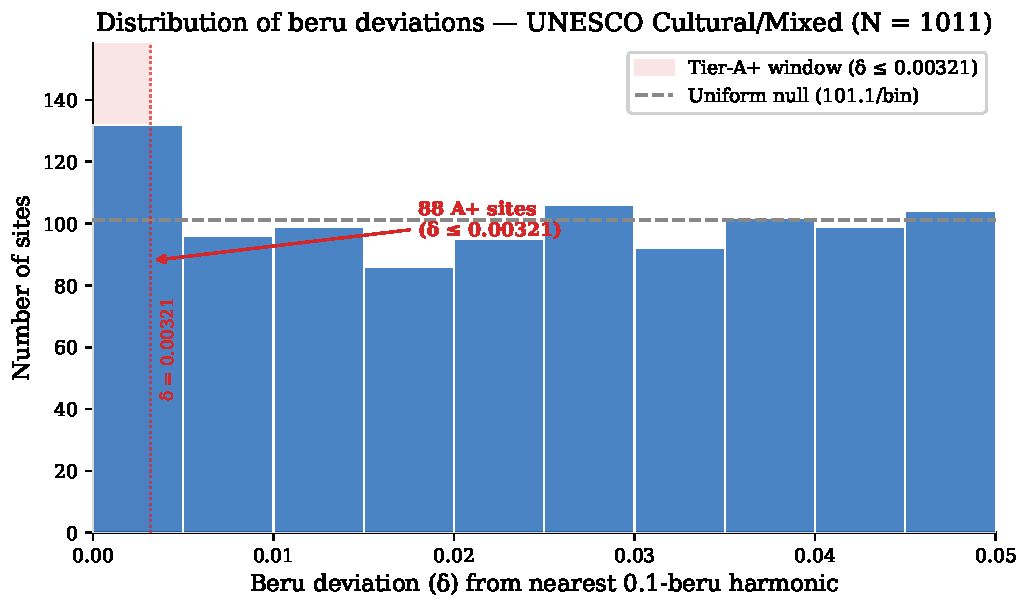
\includegraphics[width=0.9\textwidth]{../figures/fig_devhist}
\caption{Harmonic deviation distribution for the full UNESCO corpus
  ($N = \NclusterTotal$) under the selected 3\degr{} frame. The shaded
  region marks the Tier-A+ window
  ($\delta \leq \ApThreshDeg\degr{}$); the dashed line marks the
  \NullRateAp{} geometric null. The first-bin excess is the
  within-frame structure that Stages~5--7 evaluate. As shown in
  Section~\ref{sec:boundary}, the corresponding invariant test on raw
  longitudes is null.}
\label{fig:devhist}
\end{figure*}

\textbf{Empirical observation.} The full corpus has a Tier-A+ rate of
\clusterApRate\% ($\NclusterAp/\NclusterTotal$; Clopper-Pearson 95\%
CI [\clusterApCIlo\%, \clusterApCIhi\%]) against the \NullRateAp{}
geometric null (Figure~\ref{fig:devhist}). The within-frame enrichment
is $\clusterEnrichAp\times$ the null rate. This is the weak
selected-frame signal audited in the remainder of the paper.

\textbf{Test~1 (dome von~Mises mixture, exploratory subset).} A
two-component von~Mises/uniform mixture fit to the dome sub-corpus
($N = \NcircTotal$) yields $\hat{w} = \targetedWdome$
($\approx\targetedWdomePct\%$ of dome sites concentrated at the
selected phase; $\hat{\kappa} = \targetedKdome$),
$p_{\mathrm{boot}} = \targetedPdome$ (\targetedPdomeSig{};
Holm $p_{\mathrm{adj}} = \pHolmTestOne$, \pHolmTestOneSig{}). Because
the dome keyword set was refined iteratively during analysis, this
test is exploratory subset characterisation; the Holm adjustment within
the primary family does not absorb the keyword-selection step. We
report it as descriptive of the iteratively-refined sub-corpus, not
as confirmatory inference.

\textbf{Test~2 (Spearman cluster asymmetry).}
$\rho = \spearmanDevClusterRho$, permutation
$p = \spearmanDevClusterP$ (\spearmanDevClusterPSig{};
Holm $p_{\mathrm{adj}} = \pHolmTestTwo$, \pHolmTestTwoSig{}). Nodes
drawing more sites show smaller mean deviations. This is the expected
signature when a scoring function with a smooth attractor is applied
to clustered data: density modes pull the nearest grid node toward the
modal centre, reducing the mean deviation of the cluster's members.
The result is informative about the data--scoring interaction; it is
not, on its own, evidence of a historical mechanism.

\textbf{Test~3 (phase-rotation null).} The selected reference phase
minimises the full-corpus mean harmonic deviation relative to random
grid placements ($p_{\mathrm{perm}} = \fullMeanDevPermP$,
\fullMeanDevPermPSig{}; Holm $p_{\mathrm{adj}} = \pHolmTestThree$,
\pHolmTestThreeSig{}). This is the within-frame analogue of the
Stage~2 anchor-specificity finding.

\begin{table}[!t]
\centering
\caption{Stage~4 diagnostics: within-frame tests conditional on the
  selected 3\degr{} / $\sim$35\degr{}E frame. All $p$-values are
  conditional on frame selection and do not address the unconditional
  question evaluated at Stage~5
  (Section~\ref{sec:boundary}).}
\label{tab:primary_tests}
\small
\begin{tabular}{lcrll}
\toprule
Test & $N$ & Raw $p$ & Holm $p_{\mathrm{adj}}$ & Role \\
\midrule
Test~1 (dome VM mix.)
  & \NcircTotal & \targetedPdome\textsuperscript{b}
  & \pHolmTestOne~\pHolmTestOneSig{} & Exploratory subset \\
Test~2 (Spearman $\rho$)
  & \NclusterTotal & \spearmanDevClusterP\textsuperscript{b}
  & \pHolmTestTwo~\pHolmTestTwoSig{} & Within-frame diagnostic \\
Test~3 (mean dev.)
  & \NclusterTotal & \fullMeanDevPermP\textsuperscript{b}
  & \pHolmTestThree~\pHolmTestThreeSig{} & Within-frame diagnostic \\
\bottomrule
\multicolumn{5}{p{0.9\textwidth}}{\footnotesize
  \textsuperscript{b}permutation or bootstrap $p$.
  Holm (1979) step-down \citep{holm1979simple}. Holm correction is
  applied within the conditional family; it does not absorb the
  Stage~1 spacing sweep, the Stage~2 anchor sweep, or the
  iteratively-refined keyword set used in Test~1.}
\end{tabular}
\end{table}

\textbf{Dome sub-population detail (illustrative).} As a descriptive
result, \NcircTierAp/\NcircTotal{} dome sites fall at Tier-A+
(\NcircApRate\%, $\circEnrichAp\times$; Fisher $p = \pCircApFisher$,
\pCircApFisherSig{}). Tier-A++ concentration is stronger:
\NcircTierApp/\NcircTotal{} (\NcircAppRate\%, $\circEnrichApp\times$
the \NullRateApp{} null; permutation $p = \circAppPermP$,
\pCircAppPermSig{}; bootstrap $p = \circAppBootP$,
\pCircAppBootSig{}). These figures are reported for transparency;
their interpretation is bounded by the iterative keyword construction
of the dome sub-corpus.

\paragraph{Leave-$n$-out sensitivity.}
No single A+ site drives the dome result: removing any A+ site yields
$N = \LOOdomeN$, A+$= \LOOdomeAp$, $p = \LOOdomeP$.
Leave-3-out worst case across all $\binom{\LKOnAp}{3}$ triples:
$p = \LKOworstThreeP$. The A++ sub-population: leave-3-out worst case
$p = \LKOAppworstThreeP$ (leave-2-out: $p = \LKOAppworstTwoP$).
Robustness to specific sites is not, however, robustness to the
keyword construction of the sub-corpus.

\subsection{Stage~5: Boundary-Condition Tests --- The Main Limitation}
\label{sec:boundary}

The Stage~4 results are conditional on a selected frame chosen from a
parameter sweep. The broader question --- whether the data support
3\degr{} periodicity without reference to any particular phase --- is
the question Stage~5 addresses.

The full-corpus Rayleigh test for 3\degr{} periodicity returns
$R = \fullRayleighR$ ($Z = \fullRayleighZ$,
$p_{\mathrm{perm}} = \fullRayleighPermP$, \fullRayleighPermPSig{}).
This test does not support invariant 3\degr{} periodicity in the raw
longitude distribution.

This is the main limit on interpretation. Disagreement between Stage~4
(conditional, positive) and Stage~5 (invariant, null) localises the
signal at the selected-frame level rather than validating it as
invariant periodicity. A user who reads the Stage~4 $p$-values without
the Stage~5 result would draw a stronger inference than the data
support. The audit is structured so that the Rayleigh null remains a
binding boundary condition on the conditional results.

A $\pm 0.3\%$ shift from the selected 3\degr{} spacing collapses joint
within-frame concentration across the dome sub-population. This
underscores the frame-dependence of the signal; it does not by itself
settle the choice among alternative explanations.

\subsection{Stage~6: Geographic-Concentration Nulls}
\label{sec:geo_null}

Domed monuments are concentrated in the Eurasian corridor
(\domeEurasianFraction\% in 20\degr{} to 120\degr{}E versus
\fullCorpusEurasianFraction\% of the full corpus). Two null models ask
whether this footprint, rather than any morphological-spatial
relationship, accounts for the within-frame enrichment of the dome
sub-population. Because the keyword set was iterative, these results
are treated as exploratory diagnostics.

\textbf{Null~A (within-dome bootstrap).} Drawing $N = \NcircTotal$
longitudes from the dome sites' own longitude list yields a mean
expected A+ count consistent with the observed value
($p = 0.5429$, ns). The dome enrichment is consistent with where dome
sites already are; shared geography is therefore a sufficient
alternative explanation for the subset pattern.

\textbf{Null~C (restricted geographic draw).} Drawing from all
full-corpus sites within $\pm W\degr{}$ of any dome longitude, the
dome subset nominally exceeds the broader footprint at all three
tested windows: $\pm 2\degr{}$ ($p = \geoNullDomeRestrictedPtwo$,
\geoNullDomeRestrictedPtwoSig{}); $\pm 5\degr{}$
($p = \geoNullDomeRestrictedP$, \geoNullDomeRestrictedPSig{});
$\pm 10\degr{}$ ($p = \geoNullDomeRestrictedPten$,
\geoNullDomeRestrictedPtenSig{}). These marginal results do not
survive Bonferroni correction across the three windows
($\alpha_\mathrm{adj} = 0.0167$).

\begin{figure*}[!t]
\centering
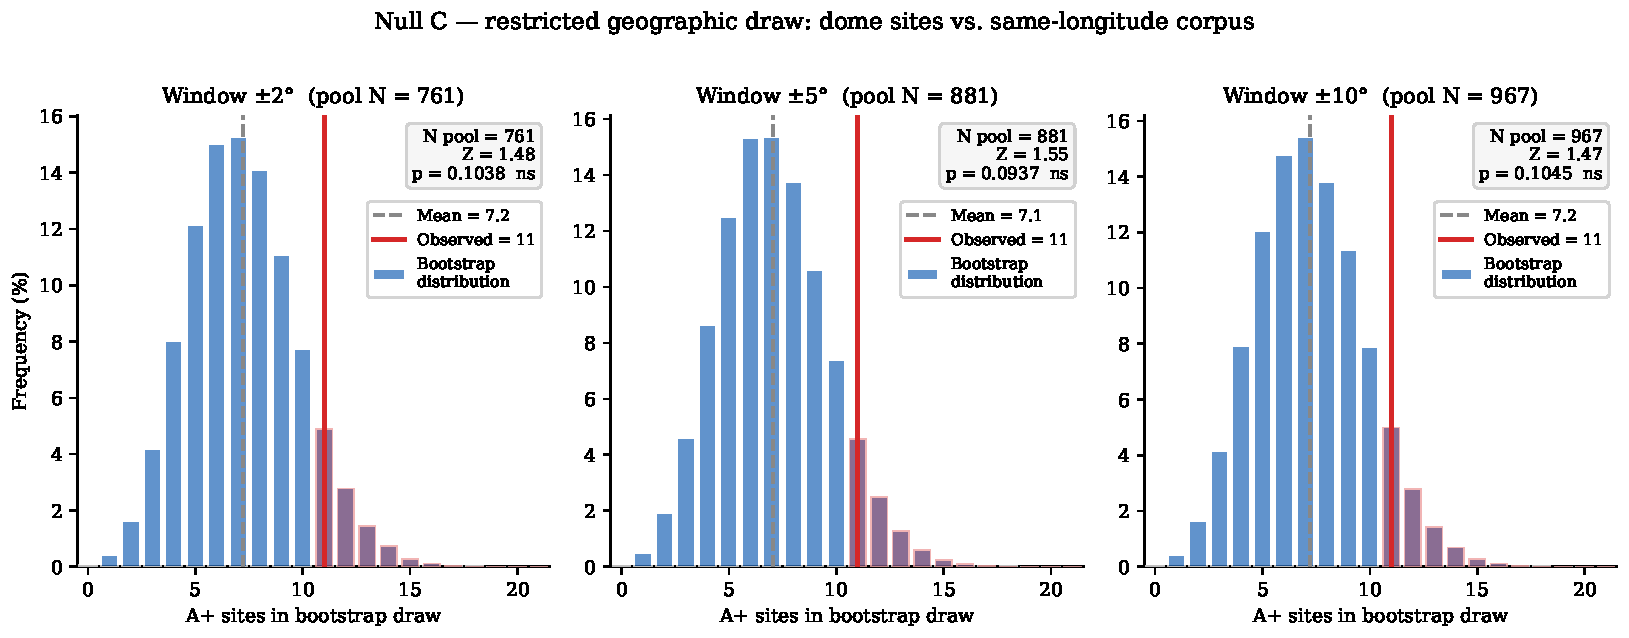
\includegraphics[width=0.9\textwidth]{../figures/fig_null_c}
\caption{Null~C bootstrap distributions for the context-validated dome
  sub-population ($N = \NcircValidated$, observed A+ $= \NcircValidatedAp$)
  at three window widths. Null~C is consistent with morphological
  specificity at the nominal level but does not survive correction for
  the three-window family.}
\label{fig:null_c}
\end{figure*}

The two nulls return ambiguous evidence on whether any morphological
specificity remains after geographic concentration is accounted for:
Null~A is consistent with footprint alone being sufficient; Null~C is
nominally consistent with residual morphological specificity but does
not survive correction. The pipeline reports both rather than forcing
a resolution; ambiguity at this stage is what the diagnostic is
designed to surface.

\paragraph{Out-of-footprint support.}
The UNESCO Americas sub-corpus ($N = \AmericasN$) shows an A+ rate of
\AmericasApRate\%, below the \NullRateAp{} null
($p = \AmericasOneSidedP$, \AmericasOneSidedStar{}, one-sided
depletion). This small sub-corpus does not support extension of the
selected-frame pattern outside the Eurasian footprint. It is not
large enough to rule out a signal elsewhere, but it gives no positive
out-of-footprint validation.

% ==============================================================================
\section{Cross-Corpus Stability under Frozen Parameters: A Same-Footprint
Check}
\label{sec:cross_corpus}
% ==============================================================================

Stage~7 asks whether the selected frame organises independently
assembled corpora at frozen parameters. Read in isolation, the answer
is yes: both stability-check corpora show elevated enrichment under
the same $(\omega, \phi)$ that selected the within-frame pattern in
UNESCO. Read in combination with Stages~5 and~6, the apparent
stability does not warrant an invariant interpretation. This section
documents both the empirical stability and the limits on what it can
mean.

\subsection{Stability Under Frozen Parameters}

\textbf{Wikidata Q180987 stupas.} Under the identical anchor, spacing,
and tier thresholds, $N = \wikiStupaTotal$ stupas yield
\wikiStupaATierCount/\wikiStupaTotal{} Tier-A sites
(\wikiStupaATierRate\%, $\wikiStupaATierEnrich\times$ null;
binomial $p\ \wikiStupaATierBinomP$, \wikiStupaATierBinomStar;
permutation $p_{\mathrm{perm}} = \wikiStupaPermP$,
\wikiStupaPermStar). Harmonic nodes with at least one Tier-A stupa
carry $\wikiStupaClusterRatio\times$ more stupa sites on average than
empty nodes. The Java/Sumatra cluster (105\degr{} to 115\degr{}E)
concentrates \wikiJavaTightATierN/\wikiJavaTightN{} sites at Tier-A
(\wikiJavaTightATierRate\%; OR $= \wikiJavaTightATierOR\times$,
$p\ \wikiJavaTightATierP$, \wikiJavaTightATierPSig{}). The Wikidata
result is partly in-sample because the corpus was used in Stage~3;
the figures are presented as a consistency check on the tier-derivation
choice and as same-footprint stability, not as independent
replication.

\textbf{OWTRAD Silk Road network.} Testing all \NOwtradDegW{}
endpoint positions across the full edge list (each city weighted by
the number of segments it connects), \NOwtradDegWApp{} fall at A++
harmonics, \NOwtradDegWAp{} at A+, and \NOwtradDegWA{} at A
($\owtradDegWAppEnrich\times$ null; $z = \zOwtradDegWApp$,
$p\ \pOwtradDegWApp$, \pOwtradDegWAppSig{} for A++; $p = \pOwtradDegWAp$,
\pOwtradDegWApSig{} for A+). A phase-shift test (random offset of the
3\degr{} grid, \NOwtradPerms{} iterations) gives
$p = \pOwtradVertexAppPhase$, \pOwtradVertexAppPhaseSig{}, consistent
with conditional enrichment at the selected phase. Harmonics
containing at least one A++ endpoint (\NOwtradAppHarmonics{} harmonics)
carry $\owtradClustDegRatio\times$ more route connectivity than
harmonics without one (\NOwtradNonAppHarmonics{} harmonics;
$p = \pOwtradClustDeg$, \pOwtradClustDegSig{}, Mann-Whitney one-tailed).
OWTRAD is out-of-sample with respect to the tier-derivation and UNESCO
keyword steps, but it shares the same Eurasian footprint.

\begin{figure*}[!t]
\centering
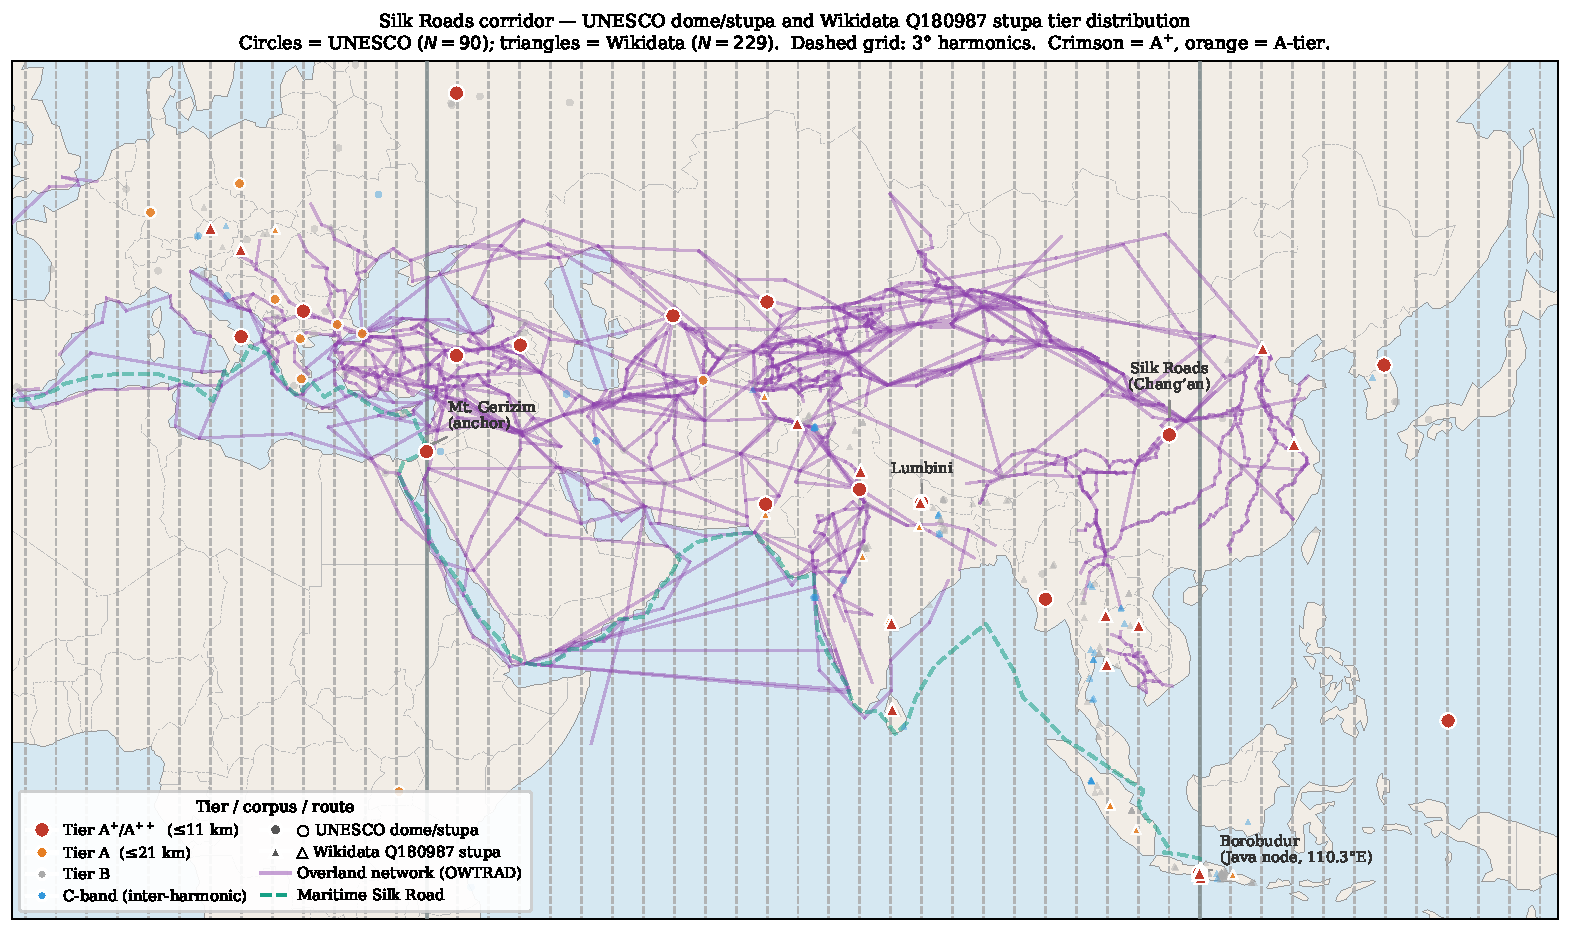
\includegraphics[width=\textwidth]{../figures/fig_geo_trail}
\caption{Tier distribution of UNESCO dome/stupa and Wikidata Q180987
  stupa sites along the Eurasian corridor, overlaid on OWTRAD attested
  trade routes \citep{ciolek2004owtrad}. The 3\degr{} harmonic grid
  (dashed) is the frame selected at Stage~2. The figure illustrates
  what cross-corpus organisation under frozen parameters \emph{looks
  like} when the test corpora share geographic footprint with the
  primary corpus. Section~\ref{sec:corridor_specificity} discusses
  why this visual coherence does not, on its own, license an invariant
  interpretation.}
\label{fig:geo_trail}
\end{figure*}

\subsection{Why the Stability Is Not Independent Replication}
\label{sec:corridor_specificity}

A natural reading of the Stage~7 results is: ``three corpora,
assembled for different purposes, show the same structure under
identical parameters --- this must reflect something invariant.''
The audit asks what would be needed for that reading to become
confirmatory. Three constraints prevent that inference here.

\textbf{Constraint 1: The invariant test is null.} The Rayleigh test
on raw longitudes returns
$p_{\mathrm{perm}} = \fullRayleighPermP$. The cross-corpus stability
is observed under the selected frame; it does not validate as an
invariant-period signal.

\textbf{Constraint 2: Out-of-footprint support is lacking.} The
Americas sub-corpus gives $p = \AmericasOneSidedP$ for one-sided
depletion. This does not rule out a signal elsewhere, but it does not
support extension beyond the footprint shared by the three positive
corpora.

\textbf{Constraint 3: All three corpora share footprint.} The Wikidata
stupa corpus and the OWTRAD route network both sit in the same
Eurasian corridor as the bulk of UNESCO Cultural inscriptions
(Section~\ref{sec:data}). Under that condition, any frame that places
lattice nodes near dense regions of the corridor may produce elevated
enrichment in any of the three corpora. Cross-corpus agreement of this
kind is same-footprint stability under a single representational choice
on three views of a common spatial concentration, not independent
replication of an invariant phenomenon.

\paragraph{Anchor-specificity check.} A reader might object that not
every anchor produces the observed enrichment, citing the Stage~2
finding that Mecca ($p = \pMeccaAnchor$), Mt.~Meru
($p = \pMeruAnchor$), and Mt.~Kailash ($p = \pKailashAnchor$) all
return non-significant conditional $p$-values in UNESCO under the
3\degr{} frame. This is correct, and it is one reason the selected
frame is an empirical object worth auditing. It does not, however,
bear the inferential weight a strong reading would require. The
35\degr{}E corridor was selected by the maximum-over-anchors search
because, given the 3\degr{} spacing, it places lattice nodes near dense
regions of the Eurasian corridor. That corridor specificity is
consistent with a geographic-fitting mechanism as a sufficient
alternative explanation.

\subsection{Scope of the Stability Finding}
\label{sec:cross_corpus_scope}

All three corpora are concentrated in the Eurasian corridor. The
worked example therefore cannot, on its own data, distinguish two
explanations of the cross-corpus stability:
\begin{enumerate}
  \item the selected frame captures something specific to the
        3\degr{} spacing and $\sim$35\degr{}E phase that goes beyond
        Eurasian corridor geography;
  \item the three corpora share enough geographic structure that any
        frame fitting one will fit the others, and shared geography
        is sufficient.
\end{enumerate}
The Stage~5 invariant null, the Stage~6 Americas result, and the
partial in-sample status of the Wikidata check prevent (1) from
becoming confirmatory. The honest summary is therefore: the worked
example contains a weak selected-frame signal, but the present tests
do not warrant an invariant interpretation; shared geography plus frame
selection is a sufficient alternative explanation for the observed
same-frame behaviour.

\paragraph{What would change the conclusion.} Two complementary forms
of evidence would be required to revisit (1). First, a heritage
corpus assembled outside the Eurasian corridor --- for example,
national registers from sub-Saharan Africa, the Pacific, or
Mesoamerica --- analysed at frozen parameters by an independent team
using the deposited code, with elevated enrichment that mirrored the
in-corridor result. Second, an invariant test (Stage~5) that returned
positive on the combined corpus, supporting periodicity rather than
phase-fit at a particular anchor. Neither is available in the present
data; we identify both as the priority follow-up tests, and neither
has been carried out.

\paragraph{A note on pre-registration.} Conventional pre-registration
infrastructure (OSF, AsPredicted) is well-suited to controlled
experimental designs and less well-suited to single-investigator
spatial-analysis pipelines that depend on iterative parameter
characterisation. The present work substitutes a frozen Zenodo
deposit (DOI: 10.5281/zenodo.19938283, v1.6.0) of the analysis code
and selected parameters. Independent application of the deposited
pipeline to corpora outside the Eurasian footprint, by a different
team, is the pre-registration analogue this design supports. The
substitution is imperfect (the deposit is contemporaneous with the
present analysis, not strictly antecedent), and it should be read as
such.

% ==============================================================================
\section{Discussion}
\label{sec:discussion}
% ==============================================================================

\subsection{What the Pipeline Distinguishes}

The worked example separates three claims that prior studies of
spatial periodicity have tended to conflate.

\emph{Within-frame concentration.} The selected frame organises the
UNESCO corpus and two related datasets in a way that random
permutations of the same frame do not (Tests~1--3, all conditional on
the selected frame, surviving Holm correction within the conditional
family). This is a genuine property of the data \emph{under the
chosen representation}.

\emph{No validation as invariant periodicity.} The full-corpus Rayleigh
test is null
($p_{\mathrm{perm}} = \fullRayleighPermP$). The within-frame
concentration does not extend to an invariant 3\degr{} period in raw
longitude. The pipeline distinguishes these two statuses by design,
and the second status limits interpretation.

\emph{Same-footprint cross-corpus stability.} The same frame produces
elevated enrichment in three Eurasian corpora at frozen parameters but
not at other reference longitudes. This is interesting under the chosen
representation, but it is consistent with a shared-geography account
and is not separable from that account on the present data.

\subsection{Mechanism}

The within-frame concentration can be explained by the interaction of
geographic clustering, the harmonic-deviation scoring function, and
frame selection. The UNESCO corpus is clustered along the Eurasian
corridor; the parameter sweep selects a frame that places lattice
nodes near dense regions of that clustering; the scoring function
rewards proximity to those nodes. This interaction is sufficient as an
alternative explanation for stable within-frame structure without any
stronger historical mechanism.

The same explanation also accounts for why cross-corpus stability
appears when test corpora share footprint with the primary corpus. The
Americas result does not support extension outside that footprint. The
paper therefore leaves the signal unresolved rather than assigning it
to a stronger historical mechanism.

\subsection{Comparison to Prior Approaches}

The pipeline addresses specific weaknesses of prior work.
\citet{thom1967} and \citet{kendall1974} used investigator-assembled
site lists; this pipeline uses externally curated corpora.
\citet{freeman1976} criticised ad hoc unit choices; this pipeline
sweeps over candidate units and reports the selection. Prior studies
rarely distinguished frame-dependent structure from invariant
periodicity; the pipeline's Stage~5 makes that distinction explicit
and visible. Prior studies also did not implement cross-corpus
stability checks at frozen parameters; the present worked example
shows why such checks, when they are not paired with invariant tests
and out-of-footprint validation, can be overinterpreted.

The general issue --- analyses that survive every check the analyst
chose to run, but reflect researcher degrees of freedom rather than
the underlying phenomenon --- is articulated for the broader social
and biomedical literature by \citet{gelmanloken2014}. The present
contribution applies that diagnostic stance to the specific structure
of spatial heritage analysis.

% ==============================================================================
\section{Implications for Practice}
\label{sec:practice}
% ==============================================================================

The worked example yields four practical recommendations for spatial
analysis of cultural heritage data.

\textbf{Report the search.} State how many frames, phases, spacings,
anchors, or thresholds were considered, and at what resolution.
Distinguish frame selection from subsequent diagnostics. When the
same data select the frame and test it, the resulting $p$-values are
conditional on the selected frame and should be labelled as such.
Holm or Bonferroni adjustment within a conditional family does not
absorb the prior selection step; that step requires its own treatment
(maximum-over-search permutation, or hold-out).

\textbf{Run an invariant test, and report its limit.} A coordinate-aligned
result should always be checked against at least one method that does
not assume the selected reference frame. The Rayleigh test on raw
longitudes is the canonical choice for periodicity claims. When the
invariant test is null and the within-frame test is positive, the
honest summary is that the result remains selected-frame structure
under the present tests. The within-frame $p$-values do not generalise
across that boundary.

\textbf{Distinguish same-footprint from out-of-footprint cross-corpus
checks.} When multiple corpora are available, freeze the selected
frame and apply it to each --- but report which corpora share
geographic footprint with the primary corpus and which do not.
Same-footprint agreement is shared-representation stability, not
independent replication. Out-of-footprint corpora are the genuine
validation check. If only same-footprint corpora are available
(as in the present worked example), the stability stage should be
labelled as a within-domain consistency check, not as cross-corpus
replication.

\textbf{Audit corpus structure.} Geographic clustering, corpus
overlap, partial in-sample use of stability-check corpora (e.g.,
through tier derivation), and iterative keyword selection should all
be treated as part of the inferential design. When multiple corpora
share geographic structure, cross-corpus consistency of frame-fitted
results may be expected; it should not carry the
inferential weight that ``independent replication'' suggests.

% ==============================================================================
\section{Conclusion}
\label{sec:conclusion}
% ==============================================================================

This paper contributes a reproducible audit pipeline for evaluating
frame-dependent structure in spatially clustered heritage data. The
pipeline's seven stages --- unit discovery, anchor characterisation,
tier-threshold derivation, within-frame diagnostics,
boundary-condition tests, geographic-concentration nulls, and
cross-corpus stability checks --- are demonstrated on the UNESCO
Cultural and Mixed corpus with stability checks against Wikidata
Q180987 stupas (within-corridor, partly in-sample) and the OWTRAD
Silk Road network (within-corridor, out-of-sample with respect to
parameter derivation).

The paper does not claim invariant 3\degr{} periodicity. It also does
not claim that the observed selected-frame signal is meaningless. The
worked example contains a weak within-frame signal: a parameter sweep
selects a frame near 3\degr{} spacing and the $\sim$35\degr{}E
corridor; the UNESCO corpus shows \NclusterAp/\NclusterTotal{}
Tier-A+ sites (\clusterApRate\% versus the \NullRateAp{} geometric
null); Stage~4 conditional diagnostics are positive; and Wikidata and
OWTRAD show related same-frame behaviour under frozen parameters.
Those facts locate a real selected-frame pattern for audit.

The pattern is not strong enough, independent enough, or invariant
enough to support a substantive claim of spatial periodicity. The
full-corpus Rayleigh test is null
($p_{\mathrm{perm}} = \fullRayleighPermP$), the Americas sub-corpus
does not support extension outside the Eurasian footprint, the dome
subset is exploratory because the keyword filter was iterative, and
the positive cross-corpus checks share the same broad geography as the
primary corpus. Shared geography plus frame selection is therefore a
sufficient alternative explanation for the observed stability.

The correct status of the result is weak, frame-dependent,
geographically confounded, and not validated as invariant. Future
validation would require preregistered or otherwise frozen-parameter
tests on genuinely out-of-footprint heritage corpora, ideally by an
independent team using the deposited code, together with a positive
invariant test. Until such evidence exists, the 3\degr{} /
$\sim$35\degr{}E result should be treated as a non-confirmatory worked
example of how weak selected-frame signals can arise and how they can
be audited without being overinterpreted. All code, data, and
reproduction instructions are archived at Zenodo
(DOI: \url{https://doi.org/10.5281/zenodo.19938283}, v1.6.0).

% ==============================================================================
%  SUPPLEMENTARY NOTE
% ==============================================================================

\paragraph{Data and code availability.}
\label{sec:data_code}
All analysis scripts, data files, and reproduction instructions are
archived at Zenodo (DOI: \url{https://doi.org/10.5281/zenodo.19938283},
v1.6.0). The pipeline regenerates all statistics and LaTeX macros from
raw data without manual editing
(\texttt{bash manuscript/reproduce\_all\_macros.sh}). Full audit files,
keyword lists, and supplementary figures are provided in
Supplementary~S1.

% ==============================================================================
%  APPENDIX
% ==============================================================================

\appendix

\section{Tier-Threshold Sensitivity}
\label{app:tier_sensitivity}

A log-scale null-rate sweep across \logSweepNtaus{} thresholds shows
that the dome within-frame pattern is not limited to the specific
tier width: \logSweepNsig{} of \logSweepNtaus{} thresholds reach
$p < 0.05$ for the dome subset; dome OR ranges
\logSweepMinEnrichCanon{}$\times$--\logSweepMaxEnrichCanon{}$\times$
across the three canonical tiers. Within $\pm$1 log-decade of the A+
threshold, \logSweepAregionNsig{} of \logSweepAregionNtaus{}
thresholds meet the nominal $p < 0.05$ threshold. As elsewhere, these
results are conditional on the selected $(\omega, \phi)$ frame and do
not generalise to the unconditional question
(Section~\ref{sec:boundary}).

\section{Von~Mises Mixture Characterisation}
\label{app:vonmises}

A von~Mises~+ uniform mixture fitted to the harmonic phase deviations
of the stability-check corpora under the selected frame provides
within-frame dispersion estimates used for tier-threshold derivation
(Stage~3): Wikidata Q180987 stupas ($N = \vmNStupa{}$):
$\hat{\kappa} = \vmKappaStupa{}$, $\hat{w} = \vmMixtureWeightStupa{}$,
$\hat{\sigma} = \vmSigmaDegStupa{}^\circ$. OWTRAD route nodes
($N = \vmNOwtrad{}$): $\hat{\kappa} = \vmKappaOwtrad{}$,
$\hat{w} = \vmMixtureWeightOwtrad{}$,
$\hat{\sigma} = \vmSigmaDegOwtrad{}^\circ$. $N$-weighted pooled
$\hat{\sigma} = \vmSigmaDegPooled{}^\circ$; $\kappa$ ratio
$= \vmKappaRatio{}$ across corpora. Tier boundaries correspond to
$0.25\hat{\sigma}$, $0.50\hat{\sigma}$, and $1.00\hat{\sigma}$ of the
stupa corpus dispersion.

\section{Keyword Audit}
\label{app:keywords}

\NcircKeywords{} morphological keywords from four roots
(\textit{stupa/stupas}, \textit{tholos}, \textit{dome/domed/domes},
\textit{spherical}) matched as whole words against site names, XML
descriptions, and extended OUV text. Context-validation for ambiguous
terms: Gate~1 (\NdomeGateNeg{} negative patterns) rejects
non-architectural uses; Gate~2 (\NdomeGatePos{} positive patterns)
requires architectural confirmation. Seven sites rejected in the
context-validated subset: Hiroshima Peace Memorial, Richtersveld,
Gyeongju, Vi\~{n}ales Valley, Rock Islands Southern Lagoon,
Uluru--Kata Tju\d{t}a, and Diqu\'{i}s Stone Spheres. The keyword set
was refined iteratively during analysis; results from the dome
sub-corpus are accordingly hypothesis-generating, as flagged in
Sections~\ref{sec:dome_subset} and \ref{sec:diagnostics}. Full
site-by-site audit in the Zenodo archive \citep{tenenbaum2026audit}.

% ==============================================================================
%  REFERENCES
% ==============================================================================

\begin{thebibliography}{99}

\bibitem[Ciolek(2004)]{ciolek2004owtrad}
Ciolek, T.~M. (2004).
\textit{Old World Trade Routes (OWTRAD) Project}.
Asia Pacific Research Online.
\url{http://www.ciolek.com/OWTRAD/DATA/tmcOWTRAD.html}

\bibitem[Freeman(1976)]{freeman1976}
Freeman, P.~R. (1976).
A Bayesian analysis of the Megalithic yard.
\textit{Journal of the Royal Statistical Society, Series A}, 139(1),
20--55.

\bibitem[Gelman \& Loken(2014)]{gelmanloken2014}
Gelman, A. \& Loken, E. (2014).
The statistical crisis in science.
\textit{American Scientist}, 102(6), 460--465.

\bibitem[Holm(1979)]{holm1979simple}
Holm, S. (1979).
A simple sequentially rejective multiple test procedure.
\textit{Scandinavian Journal of Statistics}, 6(2), 65--70.

\bibitem[Kendall(1974)]{kendall1974}
Kendall, D.~G. (1974).
Hunting quanta.
\textit{Philosophical Transactions of the Royal Society A},
276(1257), 231--266.

\bibitem[Magli(2013)]{magli2013}
Magli, G. (2013).
\textit{Architecture, Astronomy and Sacred Landscape in Ancient Egypt}.
Cambridge University Press.

\bibitem[Magli(2016)]{magli2016}
Magli, G. (2016).
\textit{Archaeoastronomy: Introduction to the Science of Stars and
Stones}.
Springer.

\bibitem[Ruggles(1999)]{ruggles1999astronomy}
Ruggles, C.~L.~N. (1999).
\textit{Astronomy in Prehistoric Britain and Ireland}.
Yale University Press.

\bibitem[Ruggles \& Cotte(2010)]{ruggles2010icomos}
Ruggles, C.~L.~N. \& Cotte, M. (Eds.) (2010).
\textit{Heritage Sites of Astronomy and Archaeoastronomy in the Context
of the UNESCO World Heritage Convention: A Thematic Study}.
ICOMOS / IAU.

\bibitem[Ruggles(2015)]{ruggles2015handbook}
Ruggles, C.~L.~N. (Ed.) (2015).
\textit{Handbook of Archaeoastronomy and Ethnoastronomy}.
Springer.

\bibitem[Silva \& Steele(2020)]{silva2020statistical}
Silva, F. \& Steele, J. (2020).
Statistical approaches to detecting archaeoastronomical alignments.
In C.~Ruggles (Ed.), \textit{Handbook of Archaeoastronomy and
Ethnoastronomy}, 295--306. Springer.

\bibitem[Tenenbaum(2026)]{tenenbaum2026audit}
Tenenbaum, S. (2026).
Harmonic alignment audit data: UNESCO World Heritage, Wikidata stupas,
and OWTRAD route network [Data set].
Zenodo. \url{https://doi.org/10.5281/zenodo.19938283}

\bibitem[Thom(1967)]{thom1967}
Thom, A. (1967).
\textit{Megalithic Sites in Britain}.
Oxford University Press.

\bibitem[UNESCO(2024)]{unescowhc2024xml}
UNESCO World Heritage Centre (2024).
World Heritage List [XML dataset].
\url{https://whc.unesco.org/en/syndication}

\end{thebibliography}

\end{document}
